\documentclass{article}

% if you need to pass options to natbib, use, e.g.:
%     \PassOptionsToPackage{numbers, compress}{natbib}
% before loading neurips_2020

% ready for submission
% \usepackage{neurips_2020}

% to compile a preprint version, e.g., for submission to arXiv, add add the
% [preprint] option:
%     \usepackage[preprint]{neurips_2020}

% to compile a camera-ready version, add the [final] option, e.g.:
%     \usepackage[final]{neurips_2020}

% to avoid loading the natbib package, add option nonatbib:
\usepackage{iclr2021_conference,times}
% Optional math commands from https://github.com/goodfeli/dlbook_notation.
%%%%% NEW MATH DEFINITIONS %%%%%

\usepackage{amsmath,amsfonts,bm}

% Mark sections of captions for referring to divisions of figures
\newcommand{\figleft}{{\em (Left)}}
\newcommand{\figcenter}{{\em (Center)}}
\newcommand{\figright}{{\em (Right)}}
\newcommand{\figtop}{{\em (Top)}}
\newcommand{\figbottom}{{\em (Bottom)}}
\newcommand{\captiona}{{\em (a)}}
\newcommand{\captionb}{{\em (b)}}
\newcommand{\captionc}{{\em (c)}}
\newcommand{\captiond}{{\em (d)}}

% Highlight a newly defined term
\newcommand{\newterm}[1]{{\bf #1}}


% Figure reference, lower-case.
\def\figref#1{figure~\ref{#1}}
% Figure reference, capital. For start of sentence
\def\Figref#1{Figure~\ref{#1}}
\def\twofigref#1#2{figures \ref{#1} and \ref{#2}}
\def\quadfigref#1#2#3#4{figures \ref{#1}, \ref{#2}, \ref{#3} and \ref{#4}}
% Section reference, lower-case.
\def\secref#1{section~\ref{#1}}
% Section reference, capital.
\def\Secref#1{Section~\ref{#1}}
% Reference to two sections.
\def\twosecrefs#1#2{sections \ref{#1} and \ref{#2}}
% Reference to three sections.
\def\secrefs#1#2#3{sections \ref{#1}, \ref{#2} and \ref{#3}}
% Reference to an equation, lower-case.
\def\eqref#1{equation~\ref{#1}}
% Reference to an equation, upper case
\def\Eqref#1{Equation~\ref{#1}}
% A raw reference to an equation---avoid using if possible
\def\plaineqref#1{\ref{#1}}
% Reference to a chapter, lower-case.
\def\chapref#1{chapter~\ref{#1}}
% Reference to an equation, upper case.
\def\Chapref#1{Chapter~\ref{#1}}
% Reference to a range of chapters
\def\rangechapref#1#2{chapters\ref{#1}--\ref{#2}}
% Reference to an algorithm, lower-case.
\def\algref#1{algorithm~\ref{#1}}
% Reference to an algorithm, upper case.
\def\Algref#1{Algorithm~\ref{#1}}
\def\twoalgref#1#2{algorithms \ref{#1} and \ref{#2}}
\def\Twoalgref#1#2{Algorithms \ref{#1} and \ref{#2}}
% Reference to a part, lower case
\def\partref#1{part~\ref{#1}}
% Reference to a part, upper case
\def\Partref#1{Part~\ref{#1}}
\def\twopartref#1#2{parts \ref{#1} and \ref{#2}}

\def\ceil#1{\lceil #1 \rceil}
\def\floor#1{\lfloor #1 \rfloor}
\def\1{\bm{1}}
\newcommand{\train}{\mathcal{D}}
\newcommand{\valid}{\mathcal{D_{\mathrm{valid}}}}
\newcommand{\test}{\mathcal{D_{\mathrm{test}}}}

\def\eps{{\epsilon}}


% Random variables
\def\reta{{\textnormal{$\eta$}}}
\def\ra{{\textnormal{a}}}
\def\rb{{\textnormal{b}}}
\def\rc{{\textnormal{c}}}
\def\rd{{\textnormal{d}}}
\def\re{{\textnormal{e}}}
\def\rf{{\textnormal{f}}}
\def\rg{{\textnormal{g}}}
\def\rh{{\textnormal{h}}}
\def\ri{{\textnormal{i}}}
\def\rj{{\textnormal{j}}}
\def\rk{{\textnormal{k}}}
\def\rl{{\textnormal{l}}}
% rm is already a command, just don't name any random variables m
\def\rn{{\textnormal{n}}}
\def\ro{{\textnormal{o}}}
\def\rp{{\textnormal{p}}}
\def\rq{{\textnormal{q}}}
\def\rr{{\textnormal{r}}}
\def\rs{{\textnormal{s}}}
\def\rt{{\textnormal{t}}}
\def\ru{{\textnormal{u}}}
\def\rv{{\textnormal{v}}}
\def\rw{{\textnormal{w}}}
\def\rx{{\textnormal{x}}}
\def\ry{{\textnormal{y}}}
\def\rz{{\textnormal{z}}}

% Random vectors
\def\rvepsilon{{\mathbf{\epsilon}}}
\def\rvtheta{{\mathbf{\theta}}}
\def\rva{{\mathbf{a}}}
\def\rvb{{\mathbf{b}}}
\def\rvc{{\mathbf{c}}}
\def\rvd{{\mathbf{d}}}
\def\rve{{\mathbf{e}}}
\def\rvf{{\mathbf{f}}}
\def\rvg{{\mathbf{g}}}
\def\rvh{{\mathbf{h}}}
\def\rvu{{\mathbf{i}}}
\def\rvj{{\mathbf{j}}}
\def\rvk{{\mathbf{k}}}
\def\rvl{{\mathbf{l}}}
\def\rvm{{\mathbf{m}}}
\def\rvn{{\mathbf{n}}}
\def\rvo{{\mathbf{o}}}
\def\rvp{{\mathbf{p}}}
\def\rvq{{\mathbf{q}}}
\def\rvr{{\mathbf{r}}}
\def\rvs{{\mathbf{s}}}
\def\rvt{{\mathbf{t}}}
\def\rvu{{\mathbf{u}}}
\def\rvv{{\mathbf{v}}}
\def\rvw{{\mathbf{w}}}
\def\rvx{{\mathbf{x}}}
\def\rvy{{\mathbf{y}}}
\def\rvz{{\mathbf{z}}}

% Elements of random vectors
\def\erva{{\textnormal{a}}}
\def\ervb{{\textnormal{b}}}
\def\ervc{{\textnormal{c}}}
\def\ervd{{\textnormal{d}}}
\def\erve{{\textnormal{e}}}
\def\ervf{{\textnormal{f}}}
\def\ervg{{\textnormal{g}}}
\def\ervh{{\textnormal{h}}}
\def\ervi{{\textnormal{i}}}
\def\ervj{{\textnormal{j}}}
\def\ervk{{\textnormal{k}}}
\def\ervl{{\textnormal{l}}}
\def\ervm{{\textnormal{m}}}
\def\ervn{{\textnormal{n}}}
\def\ervo{{\textnormal{o}}}
\def\ervp{{\textnormal{p}}}
\def\ervq{{\textnormal{q}}}
\def\ervr{{\textnormal{r}}}
\def\ervs{{\textnormal{s}}}
\def\ervt{{\textnormal{t}}}
\def\ervu{{\textnormal{u}}}
\def\ervv{{\textnormal{v}}}
\def\ervw{{\textnormal{w}}}
\def\ervx{{\textnormal{x}}}
\def\ervy{{\textnormal{y}}}
\def\ervz{{\textnormal{z}}}

% Random matrices
\def\rmA{{\mathbf{A}}}
\def\rmB{{\mathbf{B}}}
\def\rmC{{\mathbf{C}}}
\def\rmD{{\mathbf{D}}}
\def\rmE{{\mathbf{E}}}
\def\rmF{{\mathbf{F}}}
\def\rmG{{\mathbf{G}}}
\def\rmH{{\mathbf{H}}}
\def\rmI{{\mathbf{I}}}
\def\rmJ{{\mathbf{J}}}
\def\rmK{{\mathbf{K}}}
\def\rmL{{\mathbf{L}}}
\def\rmM{{\mathbf{M}}}
\def\rmN{{\mathbf{N}}}
\def\rmO{{\mathbf{O}}}
\def\rmP{{\mathbf{P}}}
\def\rmQ{{\mathbf{Q}}}
\def\rmR{{\mathbf{R}}}
\def\rmS{{\mathbf{S}}}
\def\rmT{{\mathbf{T}}}
\def\rmU{{\mathbf{U}}}
\def\rmV{{\mathbf{V}}}
\def\rmW{{\mathbf{W}}}
\def\rmX{{\mathbf{X}}}
\def\rmY{{\mathbf{Y}}}
\def\rmZ{{\mathbf{Z}}}

% Elements of random matrices
\def\ermA{{\textnormal{A}}}
\def\ermB{{\textnormal{B}}}
\def\ermC{{\textnormal{C}}}
\def\ermD{{\textnormal{D}}}
\def\ermE{{\textnormal{E}}}
\def\ermF{{\textnormal{F}}}
\def\ermG{{\textnormal{G}}}
\def\ermH{{\textnormal{H}}}
\def\ermI{{\textnormal{I}}}
\def\ermJ{{\textnormal{J}}}
\def\ermK{{\textnormal{K}}}
\def\ermL{{\textnormal{L}}}
\def\ermM{{\textnormal{M}}}
\def\ermN{{\textnormal{N}}}
\def\ermO{{\textnormal{O}}}
\def\ermP{{\textnormal{P}}}
\def\ermQ{{\textnormal{Q}}}
\def\ermR{{\textnormal{R}}}
\def\ermS{{\textnormal{S}}}
\def\ermT{{\textnormal{T}}}
\def\ermU{{\textnormal{U}}}
\def\ermV{{\textnormal{V}}}
\def\ermW{{\textnormal{W}}}
\def\ermX{{\textnormal{X}}}
\def\ermY{{\textnormal{Y}}}
\def\ermZ{{\textnormal{Z}}}

% Vectors
\def\vzero{{\bm{0}}}
\def\vone{{\bm{1}}}
\def\vmu{{\bm{\mu}}}
\def\vtheta{{\bm{\theta}}}
\def\va{{\bm{a}}}
\def\vb{{\bm{b}}}
\def\vc{{\bm{c}}}
\def\vd{{\bm{d}}}
\def\ve{{\bm{e}}}
\def\vf{{\bm{f}}}
\def\vg{{\bm{g}}}
\def\vh{{\bm{h}}}
\def\vi{{\bm{i}}}
\def\vj{{\bm{j}}}
\def\vk{{\bm{k}}}
\def\vl{{\bm{l}}}
\def\vm{{\bm{m}}}
\def\vn{{\bm{n}}}
\def\vo{{\bm{o}}}
\def\vp{{\bm{p}}}
\def\vq{{\bm{q}}}
\def\vr{{\bm{r}}}
\def\vs{{\bm{s}}}
\def\vt{{\bm{t}}}
\def\vu{{\bm{u}}}
\def\vv{{\bm{v}}}
\def\vw{{\bm{w}}}
\def\vx{{\bm{x}}}
\def\vy{{\bm{y}}}
\def\vz{{\bm{z}}}

% Elements of vectors
\def\evalpha{{\alpha}}
\def\evbeta{{\beta}}
\def\evepsilon{{\epsilon}}
\def\evlambda{{\lambda}}
\def\evomega{{\omega}}
\def\evmu{{\mu}}
\def\evpsi{{\psi}}
\def\evsigma{{\sigma}}
\def\evtheta{{\theta}}
\def\eva{{a}}
\def\evb{{b}}
\def\evc{{c}}
\def\evd{{d}}
\def\eve{{e}}
\def\evf{{f}}
\def\evg{{g}}
\def\evh{{h}}
\def\evi{{i}}
\def\evj{{j}}
\def\evk{{k}}
\def\evl{{l}}
\def\evm{{m}}
\def\evn{{n}}
\def\evo{{o}}
\def\evp{{p}}
\def\evq{{q}}
\def\evr{{r}}
\def\evs{{s}}
\def\evt{{t}}
\def\evu{{u}}
\def\evv{{v}}
\def\evw{{w}}
\def\evx{{x}}
\def\evy{{y}}
\def\evz{{z}}

% Matrix
\def\mA{{\bm{A}}}
\def\mB{{\bm{B}}}
\def\mC{{\bm{C}}}
\def\mD{{\bm{D}}}
\def\mE{{\bm{E}}}
\def\mF{{\bm{F}}}
\def\mG{{\bm{G}}}
\def\mH{{\bm{H}}}
\def\mI{{\bm{I}}}
\def\mJ{{\bm{J}}}
\def\mK{{\bm{K}}}
\def\mL{{\bm{L}}}
\def\mM{{\bm{M}}}
\def\mN{{\bm{N}}}
\def\mO{{\bm{O}}}
\def\mP{{\bm{P}}}
\def\mQ{{\bm{Q}}}
\def\mR{{\bm{R}}}
\def\mS{{\bm{S}}}
\def\mT{{\bm{T}}}
\def\mU{{\bm{U}}}
\def\mV{{\bm{V}}}
\def\mW{{\bm{W}}}
\def\mX{{\bm{X}}}
\def\mY{{\bm{Y}}}
\def\mZ{{\bm{Z}}}
\def\mBeta{{\bm{\beta}}}
\def\mPhi{{\bm{\Phi}}}
\def\mLambda{{\bm{\Lambda}}}
\def\mSigma{{\bm{\Sigma}}}

% Tensor
\DeclareMathAlphabet{\mathsfit}{\encodingdefault}{\sfdefault}{m}{sl}
\SetMathAlphabet{\mathsfit}{bold}{\encodingdefault}{\sfdefault}{bx}{n}
\newcommand{\tens}[1]{\bm{\mathsfit{#1}}}
\def\tA{{\tens{A}}}
\def\tB{{\tens{B}}}
\def\tC{{\tens{C}}}
\def\tD{{\tens{D}}}
\def\tE{{\tens{E}}}
\def\tF{{\tens{F}}}
\def\tG{{\tens{G}}}
\def\tH{{\tens{H}}}
\def\tI{{\tens{I}}}
\def\tJ{{\tens{J}}}
\def\tK{{\tens{K}}}
\def\tL{{\tens{L}}}
\def\tM{{\tens{M}}}
\def\tN{{\tens{N}}}
\def\tO{{\tens{O}}}
\def\tP{{\tens{P}}}
\def\tQ{{\tens{Q}}}
\def\tR{{\tens{R}}}
\def\tS{{\tens{S}}}
\def\tT{{\tens{T}}}
\def\tU{{\tens{U}}}
\def\tV{{\tens{V}}}
\def\tW{{\tens{W}}}
\def\tX{{\tens{X}}}
\def\tY{{\tens{Y}}}
\def\tZ{{\tens{Z}}}


% Graph
\def\gA{{\mathcal{A}}}
\def\gB{{\mathcal{B}}}
\def\gC{{\mathcal{C}}}
\def\gD{{\mathcal{D}}}
\def\gE{{\mathcal{E}}}
\def\gF{{\mathcal{F}}}
\def\gG{{\mathcal{G}}}
\def\gH{{\mathcal{H}}}
\def\gI{{\mathcal{I}}}
\def\gJ{{\mathcal{J}}}
\def\gK{{\mathcal{K}}}
\def\gL{{\mathcal{L}}}
\def\gM{{\mathcal{M}}}
\def\gN{{\mathcal{N}}}
\def\gO{{\mathcal{O}}}
\def\gP{{\mathcal{P}}}
\def\gQ{{\mathcal{Q}}}
\def\gR{{\mathcal{R}}}
\def\gS{{\mathcal{S}}}
\def\gT{{\mathcal{T}}}
\def\gU{{\mathcal{U}}}
\def\gV{{\mathcal{V}}}
\def\gW{{\mathcal{W}}}
\def\gX{{\mathcal{X}}}
\def\gY{{\mathcal{Y}}}
\def\gZ{{\mathcal{Z}}}

% Sets
\def\sA{{\mathbb{A}}}
\def\sB{{\mathbb{B}}}
\def\sC{{\mathbb{C}}}
\def\sD{{\mathbb{D}}}
% Don't use a set called E, because this would be the same as our symbol
% for expectation.
\def\sF{{\mathbb{F}}}
\def\sG{{\mathbb{G}}}
\def\sH{{\mathbb{H}}}
\def\sI{{\mathbb{I}}}
\def\sJ{{\mathbb{J}}}
\def\sK{{\mathbb{K}}}
\def\sL{{\mathbb{L}}}
\def\sM{{\mathbb{M}}}
\def\sN{{\mathbb{N}}}
\def\sO{{\mathbb{O}}}
\def\sP{{\mathbb{P}}}
\def\sQ{{\mathbb{Q}}}
\def\sR{{\mathbb{R}}}
\def\sS{{\mathbb{S}}}
\def\sT{{\mathbb{T}}}
\def\sU{{\mathbb{U}}}
\def\sV{{\mathbb{V}}}
\def\sW{{\mathbb{W}}}
\def\sX{{\mathbb{X}}}
\def\sY{{\mathbb{Y}}}
\def\sZ{{\mathbb{Z}}}

% Entries of a matrix
\def\emLambda{{\Lambda}}
\def\emA{{A}}
\def\emB{{B}}
\def\emC{{C}}
\def\emD{{D}}
\def\emE{{E}}
\def\emF{{F}}
\def\emG{{G}}
\def\emH{{H}}
\def\emI{{I}}
\def\emJ{{J}}
\def\emK{{K}}
\def\emL{{L}}
\def\emM{{M}}
\def\emN{{N}}
\def\emO{{O}}
\def\emP{{P}}
\def\emQ{{Q}}
\def\emR{{R}}
\def\emS{{S}}
\def\emT{{T}}
\def\emU{{U}}
\def\emV{{V}}
\def\emW{{W}}
\def\emX{{X}}
\def\emY{{Y}}
\def\emZ{{Z}}
\def\emSigma{{\Sigma}}

% entries of a tensor
% Same font as tensor, without \bm wrapper
\newcommand{\etens}[1]{\mathsfit{#1}}
\def\etLambda{{\etens{\Lambda}}}
\def\etA{{\etens{A}}}
\def\etB{{\etens{B}}}
\def\etC{{\etens{C}}}
\def\etD{{\etens{D}}}
\def\etE{{\etens{E}}}
\def\etF{{\etens{F}}}
\def\etG{{\etens{G}}}
\def\etH{{\etens{H}}}
\def\etI{{\etens{I}}}
\def\etJ{{\etens{J}}}
\def\etK{{\etens{K}}}
\def\etL{{\etens{L}}}
\def\etM{{\etens{M}}}
\def\etN{{\etens{N}}}
\def\etO{{\etens{O}}}
\def\etP{{\etens{P}}}
\def\etQ{{\etens{Q}}}
\def\etR{{\etens{R}}}
\def\etS{{\etens{S}}}
\def\etT{{\etens{T}}}
\def\etU{{\etens{U}}}
\def\etV{{\etens{V}}}
\def\etW{{\etens{W}}}
\def\etX{{\etens{X}}}
\def\etY{{\etens{Y}}}
\def\etZ{{\etens{Z}}}

% The true underlying data generating distribution
\newcommand{\pdata}{p_{\rm{data}}}
% The empirical distribution defined by the training set
\newcommand{\ptrain}{\hat{p}_{\rm{data}}}
\newcommand{\Ptrain}{\hat{P}_{\rm{data}}}
% The model distribution
\newcommand{\pmodel}{p_{\rm{model}}}
\newcommand{\Pmodel}{P_{\rm{model}}}
\newcommand{\ptildemodel}{\tilde{p}_{\rm{model}}}
% Stochastic autoencoder distributions
\newcommand{\pencode}{p_{\rm{encoder}}}
\newcommand{\pdecode}{p_{\rm{decoder}}}
\newcommand{\precons}{p_{\rm{reconstruct}}}

\newcommand{\laplace}{\mathrm{Laplace}} % Laplace distribution

\newcommand{\E}{\mathbb{E}}
\newcommand{\Ls}{\mathcal{L}}
\newcommand{\R}{\mathbb{R}}
\newcommand{\emp}{\tilde{p}}
\newcommand{\lr}{\alpha}
\newcommand{\reg}{\lambda}
\newcommand{\rect}{\mathrm{rectifier}}
\newcommand{\softmax}{\mathrm{softmax}}
\newcommand{\sigmoid}{\sigma}
\newcommand{\softplus}{\zeta}
\newcommand{\KL}{D_{\mathrm{KL}}}
\newcommand{\Var}{\mathrm{Var}}
\newcommand{\standarderror}{\mathrm{SE}}
\newcommand{\Cov}{\mathrm{Cov}}
% Wolfram Mathworld says $L^2$ is for function spaces and $\ell^2$ is for vectors
% But then they seem to use $L^2$ for vectors throughout the site, and so does
% wikipedia.
\newcommand{\normlzero}{L^0}
\newcommand{\normlone}{L^1}
\newcommand{\normltwo}{L^2}
\newcommand{\normlp}{L^p}
\newcommand{\normmax}{L^\infty}

\newcommand{\parents}{Pa} % See usage in notation.tex. Chosen to match Daphne's book.

\DeclareMathOperator*{\argmax}{arg\,max}
\DeclareMathOperator*{\argmin}{arg\,min}

\DeclareMathOperator{\sign}{sign}
\DeclareMathOperator{\Tr}{Tr}
\let\ab\allowbreak


\usepackage[utf8]{inputenc} % allow utf-8 input
\usepackage[T1]{fontenc}    % use 8-bit T1 fonts
\usepackage{hyperref}       % hyperlinks
\usepackage{url}            % simple URL typesetting
\usepackage{booktabs}       % professional-quality tables
\usepackage{amsfonts}       % blackboard math symbols
\usepackage{nicefrac}       % compact symbols for 1/2, etc.
\usepackage{microtype}      % microtypography
\usepackage{setspace}
\usepackage{graphicx}
\usepackage{tikz}
\usepackage{multirow}
\usepackage{amsmath}
\usepackage{bbm}
\usepackage{xcolor}
\usepackage{pifont}% http://ctan.org/pkg/pifont
\usepackage{enumitem}
\usepackage[font=small,labelfont=bf]{caption}
\usepackage{sidecap}

% !TEX root = main.tex
\newcommand{\bx}{\mathbf{x}}
\newcommand{\by}{\mathbf{y}}
\newcommand{\bp}{\mathbf{p}}
\newcommand{\bh}{\mathbf{h}}
\newcommand{\bz}{\mathbf{z}}
\newcommand{\bv}{\mathbf{v}}
\newcommand{\bq}{\mathbf{q}}
\newcommand{\bk}{\mathbf{k}}
\newcommand{\be}{\mathbf{e}}
\newcommand{\bg}{\mathbf{g}}
\newcommand{\bM}{\mathbf{M}}
\newcommand{\bW}{\mathbf{W}}
\newcommand{\bw}{\mathbf{w}}
\newcommand{\bb}{\mathbf{b}}
\newcommand{\bu}{\mathbf{u}}
\newcommand{\bbR}{\mathbb{R}}
\newcommand{\bbE}{\mathbb{E}}
\newcommand{\bmm}{\mathbf{m}}
\newcommand{\bff}{\mathbf{f}}
\newcommand{\cL}{\mathcal{L}}
\newcommand{\tb}[1]{\textbf{#1}}

% \DeclareMathOperator*{\argmax}{arg\,max}
% \DeclareMathOperator*{\argmin}{arg\,min}
\DeclareMathOperator*{\DNC}{DNC}
\DeclareMathOperator*{\LSTM}{LSTM}
\DeclareMathOperator*{\RNN}{RNN}
\DeclareMathOperator*{\CNN}{CNN}
% \DeclareMathOperator*{\MLP}{MLP}
\DeclareMathOperator*{\Ber}{Ber}
\DeclareMathOperator*{\Linear}{Linear}
% \DeclareMathOperator*{\sigmoid}{sigmoid}
% \DeclareMathOperator*{\softmax}{softmax}
% \DeclareMathOperator*{\softplus}{s_{+}}
\DeclareMathOperator*{\softplusone}{s_{+}^{-1}}
% \DeclareMathOperator*{\diag}{diag}
\DeclareMathOperator*{\bbEop}{\mathbb{E}}

\newcommand{\yes}{\ding{51}}
\newcommand{\no}{\ding{55}}

\definecolor{red}{RGB}{255,73,92}
\definecolor{blue}{RGB}{37,110,255}
\definecolor{violet}{RGB}{70,35,122}
\definecolor{green}{RGB}{61,220,151}

% Symbols
\newcommand{\pie}[1]{%
\begin{tikzpicture}
 \draw (0,0) circle (1ex);\fill (1ex,0) arc (0:#1:1ex) -- (0,0) -- cycle;
\end{tikzpicture}%
}
% \newcommand{\cmark}{\ding{51}}%
% \newcommand{\xmark}{\ding{55}}%
\newcommand{\cm}{\pie{360}}%
\newcommand{\hx}{\pie{180}}%
\newcommand{\tinyhm}{\tiny\pie{180}}%
\newcommand{\xm}{\pie{0}}%

% Table commands
\newcommand{\mc}[3]{\multicolumn{#1}{#2}{#3}}
\newcommand{\mr}[2]{\multirow{#1}{*}{#2}}%

\newcommand{\ourmodel}{contextual prototypical memory}
\newcommand{\ourmodelshort}{CPM}
\newcommand{\ourchar}{RoamingOmniglot}
\newcommand{\ourroom}{RoamingRooms}
\newcommand{\ourimg}{RoamingImageNet}
% \newcommand{\OnlineMatchingNet}{Online MatchingNet}
% \newcommand{\OnlineProtoNet}{Online ProtoNet}
\newcommand{\OnlineMatchingNet}{O-MN}
\newcommand{\OnlineIMP}{O-IMP}
\newcommand{\OnlineProtoNet}{O-PN}


\newcommand{\MR}[1]{{\color{orange}MR: #1}}
% \newcommand{\MRedit}[1]{{\color{orange} [#1]}}
\newcommand{\MRedit}[1]{{\color{orange} #1}}
\newcommand{\MCM}[1]{{\color{blue} #1}}
\newcommand{\RZ}[1]{{\color{magenta}RZ: #1}}

\title{
% Continual Few-Shot Learning with \\Prototypical Contextual Memory Networks
% A Wandering Few-Shot Learner with Temporal Contextual Memory
% Roaming Room to Room: \\Online Contextualized Few-Shot Learning
Wandering Within a World: \\Online Contextualized Few-Shot Learning \\
Supplementary Materials
}

%% NOTE: when we make an arxiv version, please uncomment acknowledgement section below
\author{
  David S.~Hippocampus\\
  \thanks{Use footnote for providing further information
    about author (webpage, alternative address)---\emph{not} for acknowledging
    funding agencies.} \\
  Department of Computer Science\\
  Cranberry-Lemon University\\
  Pittsburgh, PA 15213 \\
  \texttt{hippo@cs.cranberry-lemon.edu}
}

\begin{document}

\maketitle

\begin{abstract}
    In this document we include additional dataset statistics and experimental details. We also include additional visualization to better understand the embeddings and control parameters learned by our CPM model. Note that separate video visualizations can be found in the supplementary folder.
\end{abstract}

% \section{Dataset Statistics}

% \paragraph{\ourchar{} details:}
% For the \ourchar experiments, we use sequences with maximum 150 images, from 5 environments.
% For individual environment, we use a Chinese restaurant process to sample the class distribution. In particular, the probability of sampling a new class is:
% \begin{align}
% p_\text{new} = \frac{k \alpha + \theta}{m + \theta},
% \end{align}
% where $k$ is the number of classes that we have already sampled in the environment, and $m$ is the
% total number of instances we have in the environment. $\alpha$ is set to 0.2 and $\theta$ is set to
% 1.0 for all of our experiments.

% The switching between environments is implemented by a Markov switching process. At each step in the
% sequence there is a constant probability $p_\text{switch}$ that switch to another environment. For
% all the experiments, we set $p_\text{switch}$ to 0.2.

% \paragraph{Additional \ourroom{} statistics:} 
% Statistics of the \ourroom{} is included in Table~\ref{tab:dataset_stats}, in comparison to other
% few-shot and continual learning datasets. Note that since \ourroom{} is collected from a simulated
% environment, with 90 indoor worlds consists of 1.2K panorama images and 1.22M video frames. The
% dataset contains about 6.9K random walk sequences with a maximum of 200 frames per sequence. For
% training we randomly crop 100 frames to form a training sequence. There are 7.0K unique instance
% classes.

% Plots of additional statistics of \ourroom{} are shown in Figure~\ref{fig:additionalstats}. In
% addition to the ones shown in the main paper, the instance and viewpoint also follows long tail
% distributions. The number of objects in each frame follow an exponential distribution.

% \paragraph{Semisupervised labels:}
% Here we describe how we sample the labeled vs. unlabeled flag for each example in the semisupervised
% sequences in both \ourchar{} and \ourroom{} datasets. Due to the imbalance in our class distribution
% (from both the Chinese restaurant process and real data collection), directly masking the label may
% bias the model to ignore the rare seen classes. Ideally, we would like to preserve at least one
% labeled example for each class. Therefore, we designed the following procedure.

% First, for each class $k$, suppose $m_k$ is the number of examples in the sequence that belong to
% the class. Let $\alpha$ be the target label ratio. Then the class-specific label ratio $\alpha_k$
% is:
% \begin{align}
% \alpha_k = (1 - \alpha) \exp(-0.5 (m_k - 1)) + \alpha.
% \label{eq:semisup}
% \end{align}
% We then for each class $k$, we sample a binary Bernoulli sequence based on $\Ber(\alpha_k)$. If a
% class has all zeros in the Bernoulli sequence, we flip the flag of one of the instances to 1 to make
% sure there is at least one labeled instance for each class.

% \paragraph{Dataset splits}
% We include details about our dataset splits in Table~\ref{tab:omniglotsplit} and
% \ref{tab:matterportsplit}.

% \section{Experiment Details}
% \paragraph{Network architecture:}
% For the \ourchar{} experiment we used the common 4-layer CNN for few-shot learning with 64 channels
% in each layer, resulting in a 64-d feature vector~\cite{protonet}. For the \ourroom{} experiment we
% resize the input to 120$\times$160 and we use the ResNet-12 architecture~\cite{tadam} with
% \{32,64,128,256\} channels per block. To represent the feature of the input image with an attention
% mask, we concatenate the global average pooled feature with the attention ROI feature, resulting in
% a 512d feature vector. For the contextual RNN, in both experiments we used an LSTM~\cite{lstm} with
% a 256d hidden state. 

% We use a linear layer to map from the output of the RNN to the features and control variables. We
% obtain $\gamma^{r,w}$ by adding 1.0 to the linear layer output and then applying the softplus
% activation. The bias units for $\beta^{r,w}$ are initialized to 10.0 for all of our experiments. We
% also apply the softplus activation to $\bm$ from the linear layer output.

% % !TEX root = ../main.tex
\begin{table}[t]
\iflatexml
    \begin{tabular}{ccccccc}
    \toprule
                                  & {\bf Images} & {\bf Sequences} & {\bf Classes} & {\bf Content}                  \\
    \midrule                                                                     
    Permuted MNIST~\citep{mnist}   & 60K          & -           & -          & Hand written digits          \\
    Omniglot~\citep{omniglot}      & 32.4K        & -           & 1.6K       & Hand written characters      \\
    CIFAR-100~\citep{cifar}        & 50K          & -           & 100        & Common objects               \\
    mini-ImageNet~\citep{matchingnet}& 50K        & -           & 100        & Common objects               \\
    tiered-ImageNet~\citep{fewshotssl}& 779K      & -           & 608        & Common objects               \\
    OpenLORIS  \citep{openloris}   & 98K          & -           & 69         & Small table-top obj.         \\
    CORe50  \citep{core50}         & 164.8K       & 11          & 50         & Hand-held obj.               \\
    \midrule                                                                                                          
    \ourroom{} (Ours)            & 1.22M         & 6.9K        & 7.0K       & General indoor instances     \\
    \bottomrule
    \end{tabular}
    \caption{\small Continual \& few-shot learning datasets}
    \label{tab:dataset_stats}
\else
    \vspace{-0.5in}
    \begin{center}
    \begin{small}
    \caption{\small Continual \& few-shot learning datasets}
    \label{tab:dataset_stats}
    \begin{tabular}{ccccccc}
    \toprule
                                  & {\bf Images} & {\bf Sequences} & {\bf Classes} & {\bf Content}                  \\
    \midrule                                                                     
    Permuted MNIST~\citep{mnist}   & 60K          & -           & -          & Hand written digits          \\
    Omniglot~\citep{omniglot}      & 32.4K        & -           & 1.6K       & Hand written characters      \\
    CIFAR-100~\citep{cifar}        & 50K          & -           & 100        & Common objects               \\
    mini-ImageNet~\citep{matchingnet}& 50K        & -           & 100        & Common objects               \\
    tiered-ImageNet~\citep{fewshotssl}& 779K      & -           & 608        & Common objects               \\
    OpenLORIS  \citep{openloris}   & 98K          & -           & 69         & Small table-top obj.         \\
    CORe50  \citep{core50}         & 164.8K       & 11          & 50         & Hand-held obj.               \\
    \midrule                                                                                                          
    \ourroom{} (Ours)            & 1.22M         & 6.9K        & 7.0K       & General indoor instances     \\
    \bottomrule
    \end{tabular}
    \vspace{-0.2in}
    \end{small}
    \end{center}
\fi
\end{table}


% \begin{figure}
% \centering
% % \fbox{
% 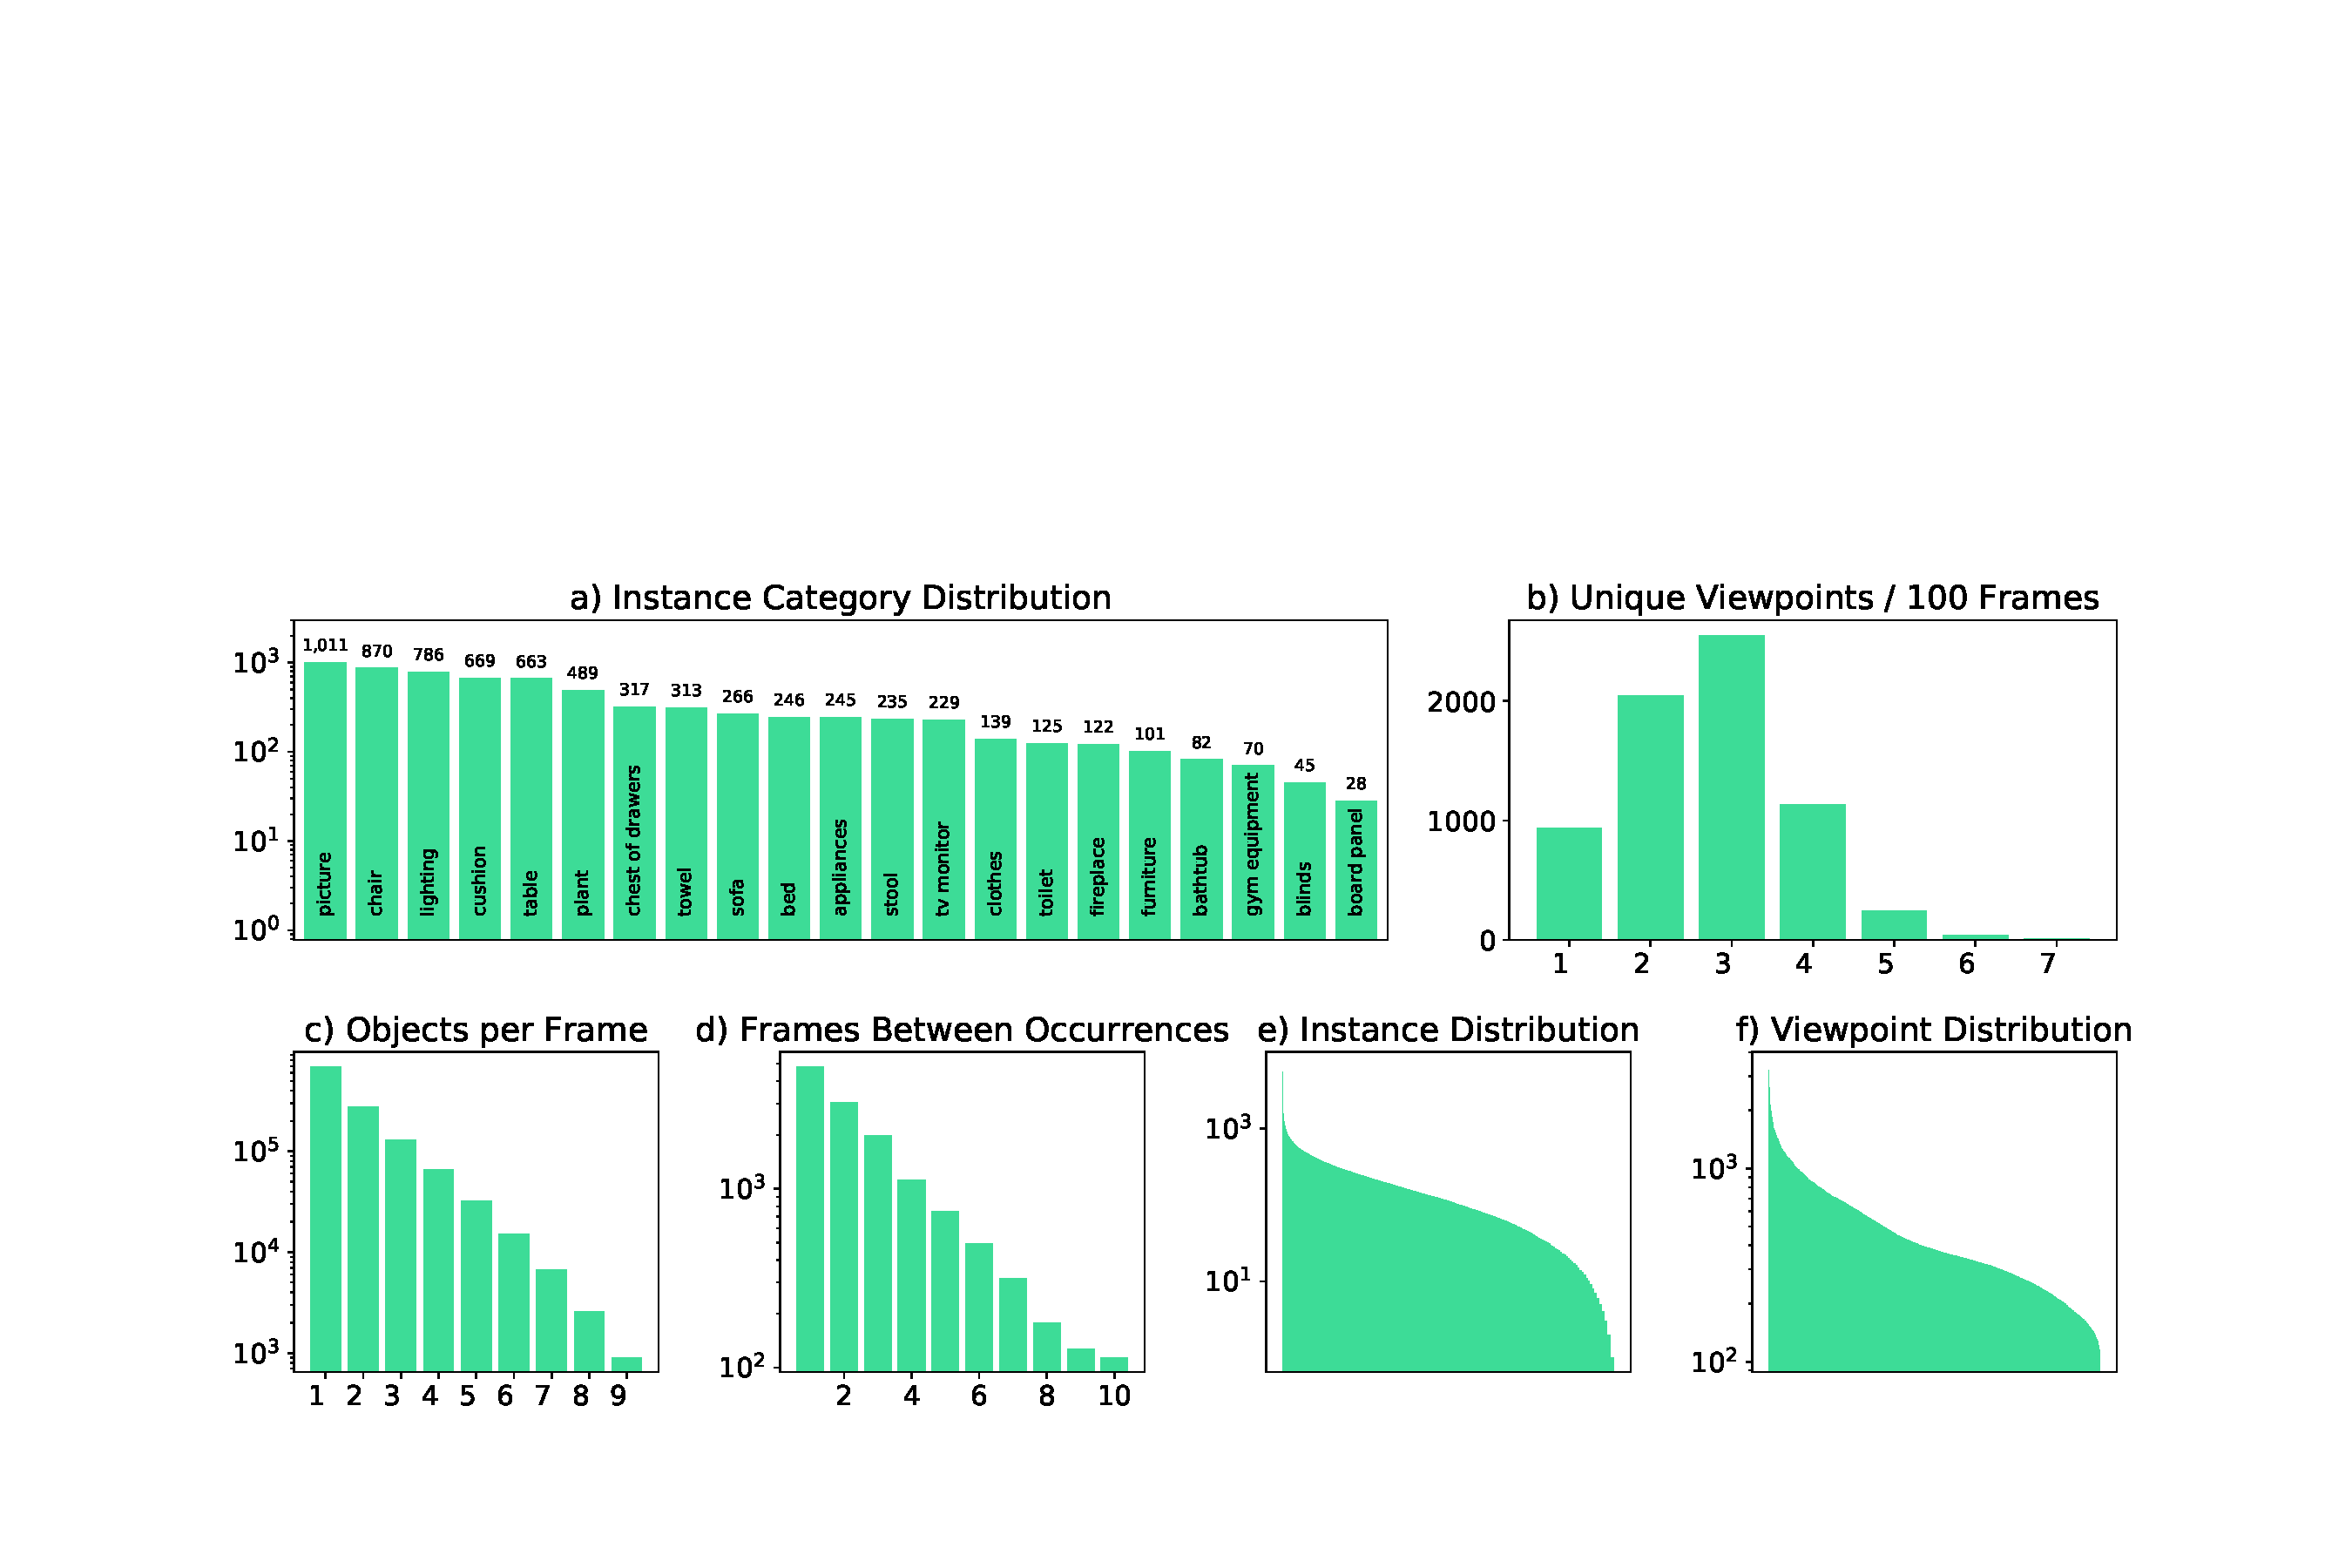
\includegraphics[width=0.95\textwidth,trim={4.5cm 3cm 4.2cm 10cm},clip]{figures/combined_catv2_counts.pdf}
% % }
% \caption{Additional statistics about our \ourroom{} dataset.}
% \label{fig:additionalstats}
% \end{figure}

% % !TEX root = ../main.tex
\begin{table}[t]
\iflatexml
    \begin{tabular}{clll}
    \toprule

    \mr{11}{Train} &
    \texttt{Angelic} &
    \texttt{Grantha} &
    \texttt{N Ko}\\
    & 
    \texttt{Aurek-Besh} &
    \texttt{Japanese (hiragana)} &
    \texttt{Malay}
    \\
    & 
    \texttt{Asomtavruli} &
    \texttt{Sanskrit} &
    \texttt{Ojibwe}
    \\
    & 
    \texttt{Korean} &
    \texttt{Arcadian} &
    \texttt{Greek}
    \\
    & 
    \texttt{Alphabet of the Magi} &
    \texttt{Blackfoot} &
    \texttt{Futurama}
    \\
    & 
    \texttt{Tagalog} &
    \texttt{Anglo-Saxon Futhorc} &
    \texttt{Braille}
    \\
    & 
    \texttt{Cyrillic} &
    \texttt{Burmese} &
    \texttt{Avesta}
    \\
    & 
    \texttt{Gujarati} &
    \texttt{Ge ez} &
    \texttt{Syriac (Estrangelo)}
    \\
    & 
    \texttt{Atlantean} &
    \texttt{Japanese (katakana)} &
    \texttt{Balinese}
    \\
    & 
    \texttt{Atemayar Qelisayer} &
    \texttt{Glagolitic} &
    \texttt{Tifinagh}
    \\
    & 
    \texttt{Latin} &
    \texttt{Inuktitut} &
    \\
    \midrule
    \mr{2}{Val} &
    \texttt{Hebrew} &
    \texttt{Mkhedruli} &
    \texttt{Armenian}\\
    & 
    \texttt{Early Aramaic} &
    \texttt{Bengali} &
    \\
    \midrule

    \mr{5}{Test} & 
    \texttt{Gurmukhi} &
    \texttt{Kannada} & 
    \texttt{Keble} \\
    &
    \texttt{Malayalam} &
    \texttt{Manipuri} &
    \texttt{Mongolian} 
    \\
    &
    \texttt{Old Church Slavonic} &
    \texttt{Oriya} &
    \texttt{Syriac (Serto)} \\
    &
    \texttt{Sylheti} &
    \texttt{Tengwar} &
    \texttt{Tibetan}\\
    &
    \texttt{ULOG}
    \\
    \bottomrule
    \end{tabular}
     \caption{\textbf{Split information for {\it \ourchar{}}}. Each column is an alphabet and we include all the characters in the alphabet in the split. Rows are continuation of lines.}
    \label{tab:omniglotsplit}
\else
    \vspace{-0.5in}
     \caption{\textbf{Split information for {\it \ourchar{}}}. Each column is an alphabet and we include all the characters in the alphabet in the split. Rows are continuation of lines.}
    \begin{center}
    \begin{small}
    \label{tab:omniglotsplit}
    \begin{tabular}{clll}
    \toprule

    \mr{11}{Train} &
    \texttt{Angelic} &
    \texttt{Grantha} &
    \texttt{N Ko}\\
    & 
    \texttt{Aurek-Besh} &
    \texttt{Japanese (hiragana)} &
    \texttt{Malay}
    \\
    & 
    \texttt{Asomtavruli} &
    \texttt{Sanskrit} &
    \texttt{Ojibwe}
    \\
    & 
    \texttt{Korean} &
    \texttt{Arcadian} &
    \texttt{Greek}
    \\
    & 
    \texttt{Alphabet of the Magi} &
    \texttt{Blackfoot} &
    \texttt{Futurama}
    \\
    & 
    \texttt{Tagalog} &
    \texttt{Anglo-Saxon Futhorc} &
    \texttt{Braille}
    \\
    & 
    \texttt{Cyrillic} &
    \texttt{Burmese} &
    \texttt{Avesta}
    \\
    & 
    \texttt{Gujarati} &
    \texttt{Ge ez} &
    \texttt{Syriac (Estrangelo)}
    \\
    & 
    \texttt{Atlantean} &
    \texttt{Japanese (katakana)} &
    \texttt{Balinese}
    \\
    & 
    \texttt{Atemayar Qelisayer} &
    \texttt{Glagolitic} &
    \texttt{Tifinagh}
    \\
    & 
    \texttt{Latin} &
    \texttt{Inuktitut} &
    \\
    \midrule
    \mr{2}{Val} &
    \texttt{Hebrew} &
    \texttt{Mkhedruli} &
    \texttt{Armenian}\\
    & 
    \texttt{Early Aramaic} &
    \texttt{Bengali} &
    \\
    \midrule

    \mr{5}{Test} & 
    \texttt{Gurmukhi} &
    \texttt{Kannada} & 
    \texttt{Keble} \\
    &
    \texttt{Malayalam} &
    \texttt{Manipuri} &
    \texttt{Mongolian} 
    \\
    &
    \texttt{Old Church Slavonic} &
    \texttt{Oriya} &
    \texttt{Syriac (Serto)} \\
    &
    \texttt{Sylheti} &
    \texttt{Tengwar} &
    \texttt{Tibetan}\\
    &
    \texttt{ULOG}
    \\
    \bottomrule
    \end{tabular}
    \end{small}
    \end{center}
\fi
\end{table}

% % !TEX root = ../main.tex
\iflatexml
\begin{table}[t]
\begin{tabular}{cc}
\toprule
\mr{12}{Train} &
\texttt{
r1Q1Z4BcV1o
JmbYfDe2QKZ
29hnd4uzFmX
ULsKaCPVFJR
E9uDoFAP3SH
}\\
&
\texttt{
8WUmhLawc2A
Uxmj2M2itWa
mJXqzFtmKg4
V2XKFyX4ASd
EU6Fwq7SyZv
}\\
&
\texttt{
gYvKGZ5eRqb
gxdoqLR6rwA
YFuZgdQ5vWj
gTV8FGcVJC9
sT4fr6TAbpF
}\\
&
\texttt{
VVfe2KiqLaN
fzynW3qQPVF
WYY7iVyf5p8
VFuaQ6m2Qom
YmJkqBEsHnH
}\\
&
\texttt{
2t7WUuJeko7
pLe4wQe7qrG
cV4RVeZvu5T
XcA2TqTSSAj
ur6pFq6Qu1A
}\\
&
\texttt{
1pXnuDYAj8r
b8cTxDM8gDG
x8F5xyUWy9e
X7HyMhZNoso
aayBHfsNo7d
}\\
&
\texttt{
TbHJrupSAjP
sKLMLpTHeUy
2azQ1b91cZZ
2n8kARJN3HM
Vvot9Ly1tCj
}\\
&
\texttt{
S9hNv5qa7GM
EDJbREhghzL
qoiz87JEwZ2
q9vSo1VnCiC
Vt2qJdWjCF2
}\\
&
\texttt{
VzqfbhrpDEA
D7G3Y4RVNrH
ZMojNkEp431
uNb9QFRL6hY
5LpN3gDmAk7
}\\
&
\texttt{
rqfALeAoiTq
e9zR4mvMWw7
yqstnuAEVhm
zsNo4HB9uLZ
JF19kD82Mey
}\\
&
\texttt{
759xd9YjKW5
wc2JMjhGNzB
rPc6DW4iMge
jh4fc5c5qoQ
HxpKQynjfin
}\\
&
\texttt{
GdvgFV5R1Z5
kEZ7cmS4wCh
vyrNrziPKCB
D7N2EKCX4Sj
PX4nDJXEHrG
}\\

\midrule

\mr{2}{Val} &
\texttt{
s8pcmisQ38h
dhjEzFoUFzH
RPmz2sHmrrY
1LXtFkjw3qL
8194nk5LbLH
}\\
&
\texttt{
jtcxE69GiFV
QUCTc6BB5sX
p5wJjkQkbXX
JeFG25nYj2p
82sE5b5pLXE
}\\
\midrule

\mr{4}{Test} & 
\texttt{
oLBMNvg9in8
r47D5H71a5s
Z6MFQCViBuw
YVUC4YcDtcY
pRbA3pwrgk9
}\\
&
\texttt{
SN83YJsR3w2
gZ6f7yhEvPG
ac26ZMwG7aT
7y3sRwLe3Va
B6ByNegPMKs
}\\
&
\texttt{
UwV83HsGsw3
VLzqgDo317F
17DRP5sb8fy
pa4otMbVnkk
5ZKStnWn8Zo
}\\
&
\texttt{
PuKPg4mmafe
Pm6F8kyY3z2
i5noydFURQK
ARNzJeq3xxb
5q7pvUzZiYa
}\\
\bottomrule
\end{tabular}
\caption{\textbf{Split information for {\it \ourroom{}}}. Each column is the ID of an indoor world. Rows are continuation of the lines.}
\label{tab:matterportsplit}
\end{table}

\begin{table}[t]
\begin{tabular}{cccc}
\toprule
Split & Worlds & Sequences & Frames \\
\midrule
Train & 60     & 4,699      &   823,444     \\
Val   & 20     &  725         &  125,823  \\
Test  & 10     &  1,547      &  271,335      \\
\midrule
Total & 90     & 6,971   & 1,220,602 \\
\bottomrule
\end{tabular}
\caption{{\it \ourroom{}} dataset split size}
\label{tab:matterportsplitsize}
\end{table}
\else
    \begin{table}[t]
    \caption{\textbf{Split information for {\it \ourroom{}}}. Each column is the ID of an indoor world. Rows are continuation of the lines.}
    \label{tab:matterportsplit}
    % \vspace{-0.5in}
    \begin{center}
    \begin{small}
    \begin{tabular}{cc}
    \toprule
    \mr{12}{Train} &
    \texttt{
    r1Q1Z4BcV1o
    JmbYfDe2QKZ
    29hnd4uzFmX
    ULsKaCPVFJR
    E9uDoFAP3SH
    }\\
    &
    \texttt{
    8WUmhLawc2A
    Uxmj2M2itWa
    mJXqzFtmKg4
    V2XKFyX4ASd
    EU6Fwq7SyZv
    }\\
    &
    \texttt{
    gYvKGZ5eRqb
    gxdoqLR6rwA
    YFuZgdQ5vWj
    gTV8FGcVJC9
    sT4fr6TAbpF
    }\\
    &
    \texttt{
    VVfe2KiqLaN
    fzynW3qQPVF
    WYY7iVyf5p8
    VFuaQ6m2Qom
    YmJkqBEsHnH
    }\\
    &
    \texttt{
    2t7WUuJeko7
    pLe4wQe7qrG
    cV4RVeZvu5T
    XcA2TqTSSAj
    ur6pFq6Qu1A
    }\\
    &
    \texttt{
    1pXnuDYAj8r
    b8cTxDM8gDG
    x8F5xyUWy9e
    X7HyMhZNoso
    aayBHfsNo7d
    }\\
    &
    \texttt{
    TbHJrupSAjP
    sKLMLpTHeUy
    2azQ1b91cZZ
    2n8kARJN3HM
    Vvot9Ly1tCj
    }\\
    &
    \texttt{
    S9hNv5qa7GM
    EDJbREhghzL
    qoiz87JEwZ2
    q9vSo1VnCiC
    Vt2qJdWjCF2
    }\\
    &
    \texttt{
    VzqfbhrpDEA
    D7G3Y4RVNrH
    ZMojNkEp431
    uNb9QFRL6hY
    5LpN3gDmAk7
    }\\
    &
    \texttt{
    rqfALeAoiTq
    e9zR4mvMWw7
    yqstnuAEVhm
    zsNo4HB9uLZ
    JF19kD82Mey
    }\\
    &
    \texttt{
    759xd9YjKW5
    wc2JMjhGNzB
    rPc6DW4iMge
    jh4fc5c5qoQ
    HxpKQynjfin
    }\\
    &
    \texttt{
    GdvgFV5R1Z5
    kEZ7cmS4wCh
    vyrNrziPKCB
    D7N2EKCX4Sj
    PX4nDJXEHrG
    }\\

    \midrule

    \mr{2}{Val} &
    \texttt{
    s8pcmisQ38h
    dhjEzFoUFzH
    RPmz2sHmrrY
    1LXtFkjw3qL
    8194nk5LbLH
    }\\
    &
    \texttt{
    jtcxE69GiFV
    QUCTc6BB5sX
    p5wJjkQkbXX
    JeFG25nYj2p
    82sE5b5pLXE
    }\\
    \midrule

    \mr{4}{Test} & 
    \texttt{
    oLBMNvg9in8
    r47D5H71a5s
    Z6MFQCViBuw
    YVUC4YcDtcY
    pRbA3pwrgk9
    }\\
    &
    \texttt{
    SN83YJsR3w2
    gZ6f7yhEvPG
    ac26ZMwG7aT
    7y3sRwLe3Va
    B6ByNegPMKs
    }\\
    &
    \texttt{
    UwV83HsGsw3
    VLzqgDo317F
    17DRP5sb8fy
    pa4otMbVnkk
    5ZKStnWn8Zo
    }\\
    &
    \texttt{
    PuKPg4mmafe
    Pm6F8kyY3z2
    i5noydFURQK
    ARNzJeq3xxb
    5q7pvUzZiYa
    }\\
    \bottomrule
    \end{tabular}
    \end{small}
    \end{center}
    \end{table}

    \begin{table}[t]
    \vspace{-0.5in}
    \caption{{\it \ourroom{}} dataset split size}
    \label{tab:matterportsplitsize}
    \begin{center}
    \begin{small}
    \begin{tabular}{cccc}
    \toprule
    Split & Worlds & Sequences & Frames \\
    \midrule
    Train & 60     & 4,699      &   823,444     \\
    Val   & 20     &  725         &  125,823  \\
    Test  & 10     &  1,547      &  271,335      \\
    \midrule
    Total & 90     & 6,971   & 1,220,602 \\
    \bottomrule
    \end{tabular}
    \end{small}
    \end{center}
    \end{table}
\fi


% \paragraph{Training details:}
% We use the Adam optimizer~\cite{adam} with initial learning rate 1e-3 for all experiments. For
% Omniglot we train the network for 40k steps with batch size of 32 with maximum sequence length 150
% across 2 GPUs and learning rate decay by 0.1$\times$ at 20k and 30k steps. For Matterport 3D we
% train for 20k steps with batch size 8 with maximum sequence length 100 across 4 GPUs and learning
% rate decay by 0.1$\times$ at 8k and 16k steps. We use BCE coeffcient $\lambda=1$  for all
% experiments. In semisupervised experiments, around 30\% examples are labeled ($\alpha = 0.3$, see
% Eq.~\ref{eq:semisup}).

% \paragraph{Data augmentation details:}
% For \ourchar{}, we pad the 28$\times$28 image to 32$\times$32 and then apply random cropping.

% For \ourroom{}, we apply random cropping in the time dimension to get a chunk of 100 frames per input example. We also apply random dropping of 5\% of the frames. We pad the 120$\times$160 images to 126 $\times$ 168 and apply random cropping in each image frame. We also randomly flip the order of the sequence (going forward or backward).

% \section{Additional Visualization of Experimental Results}

% \paragraph{Video visualization:}
% We include video visualization of \ourroom{} sequences in the supplementary zip folder. The class label is shown on the top left corner, and the CPM model prediction is right below the class label. Labeled objects are shown with red solid boxes, and unlabeled ones are shown with gray dashed boxes. Correct model predictions are colored in green whereas wrong ones are colored in red. 

% \paragraph{Prediction accuracy vs. time:}
% Figure~\ref{fig:acctimefull} shows the prediction accuracy of closed-set classes over time. We
% included supervised settings in addition to the unsupervised settings in the main paper.

% % !TEX root = ../main.tex
\begin{figure}[t]
\vspace{-0.5in}
\centering
\iflatexml
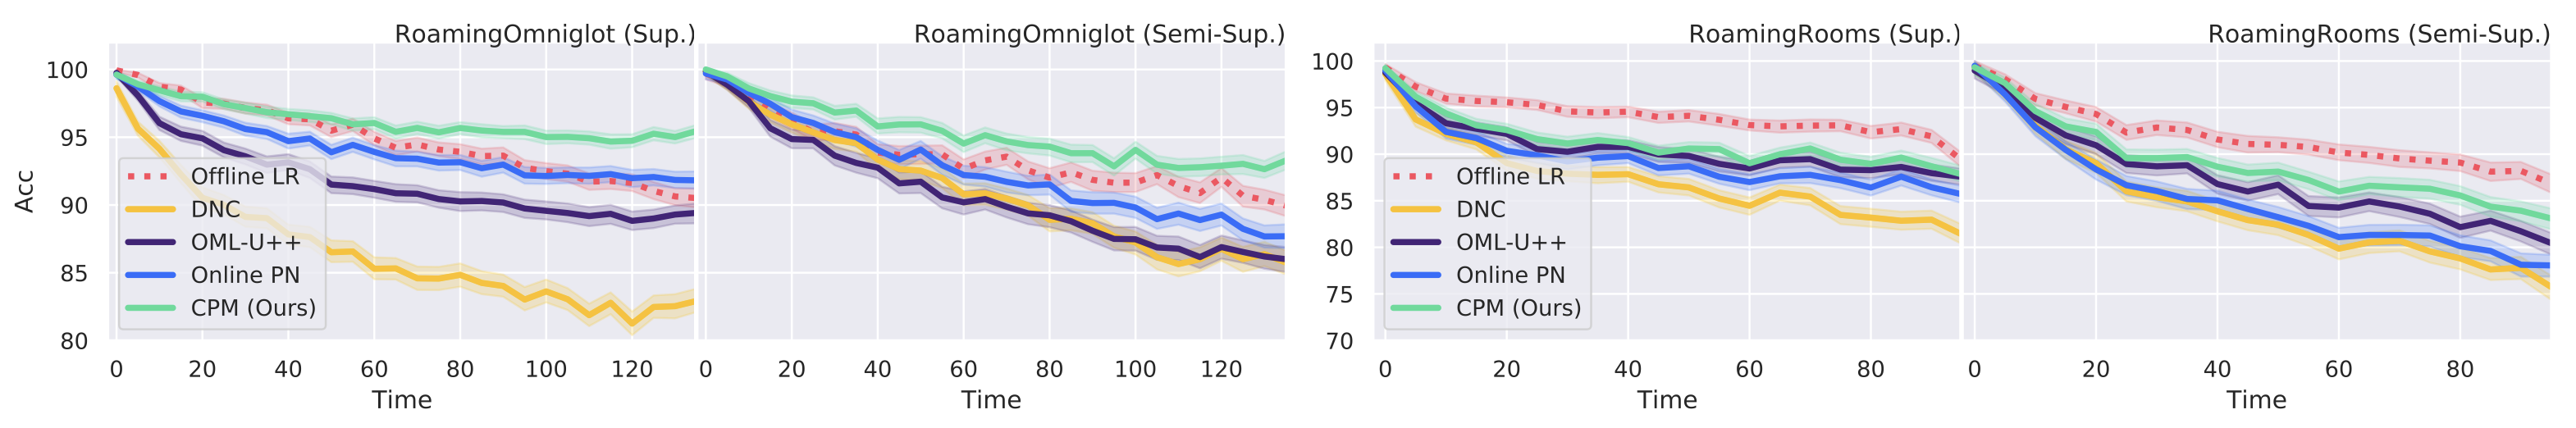
\includegraphics[width=6\linewidth]{figures/acctime_full.png}
\else
\setlength{\tabcolsep}{0pt}
\begin{tabular}{cccc}
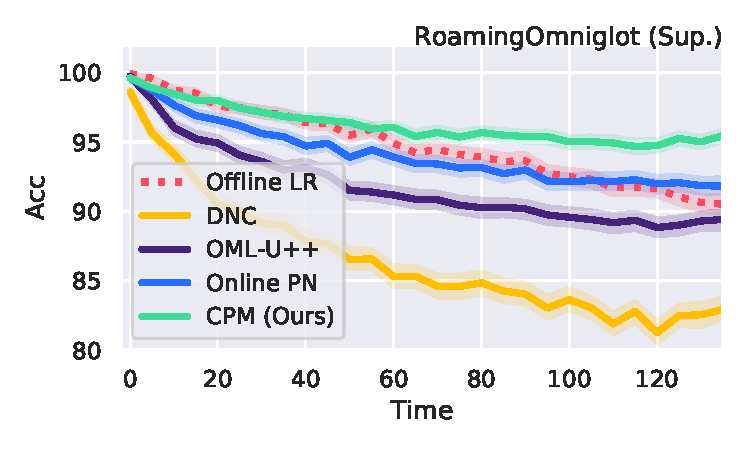
\includegraphics[height=2.4cm,trim={0.3cm 0cm 0.5cm 0},clip]{figures/omniglot-nossl-time.pdf}
&
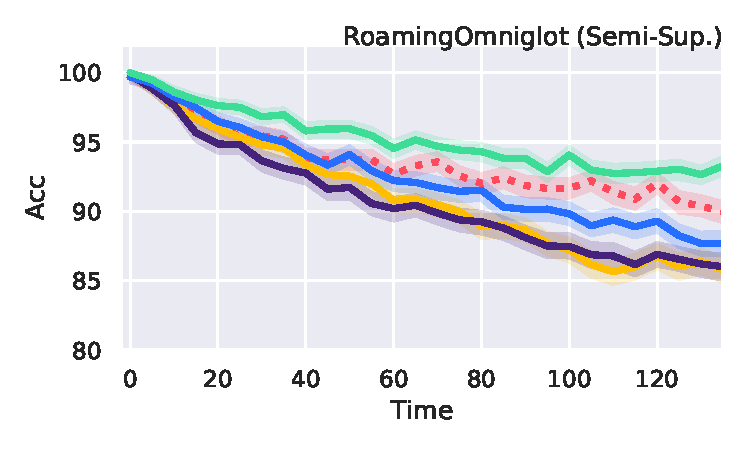
\includegraphics[height=2.4cm,trim={2cm 0cm 0cm 0},clip]{figures/omniglot-ssl-time.pdf}
&
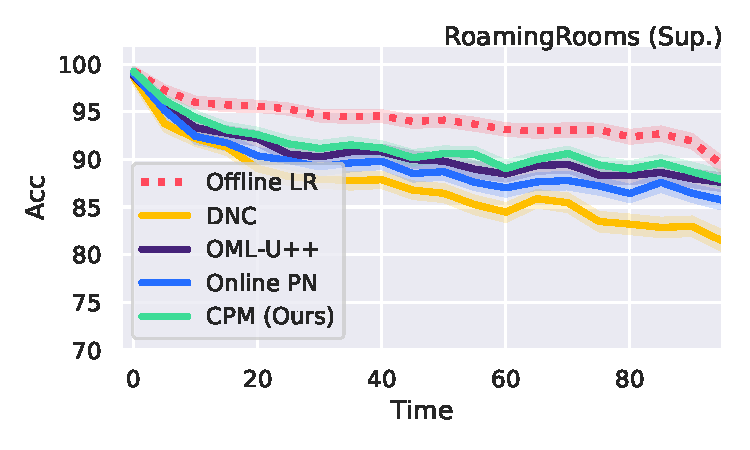
\includegraphics[height=2.4cm,trim={1cm 0cm 0.5cm 0},clip]{figures/matterport-nossl-time.pdf}
&
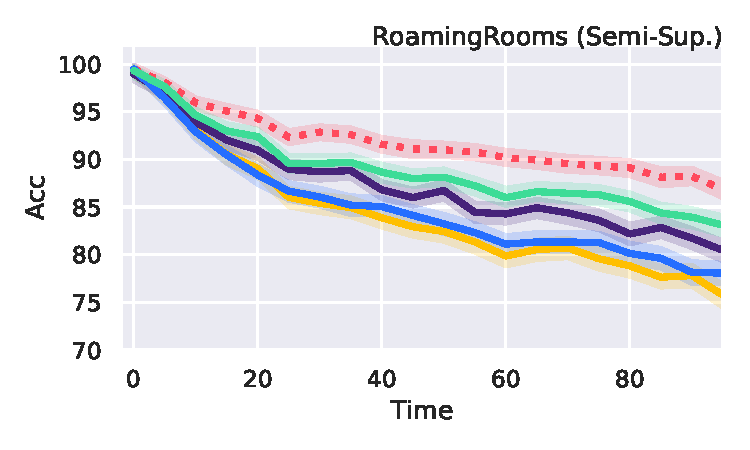
\includegraphics[height=2.4cm,trim={2cm 0cm 0cm 0},clip]{figures/matterport-ssl-time.pdf}
\\
\end{tabular}
\vspace{-0.25in}
\fi
\caption{\textbf{Few-shot classification accuracy over time.} \textbf{Left:} \ourchar{}.
\textbf{Right:} \ourroom{}. \textbf{Top:} Supervised. \textbf{Bottom:} Semi-supervised. An offline
logistic regression (Offline LR) baseline is also included, using pretrained ProtoNet features. It
is trained on all labeled examples except for the one at the current time step.}
\label{fig:acctimefull}
% \vspace{-0.25in}
\end{figure}


% \paragraph{Embedding visualization:}
% Figure~\ref{fig:tsne} shows the learned embedding of each examples in Online ProtoNet vs. our CPM
% model in \ourchar{} sequences, where colors indicate the environment ID. In Online ProtoNet, the
% example features does not reflect the temporal context, and as a result, colors are scattered across
% the space. By contrast, in the CPM embedding visualization, colors are clustered together and we see
% a smoother transition of environments in the embedding space.
% % !TEX root = ../supp.tex
\begin{figure}[t]
\centering
% \vspace{-0.2in}
\iflatexml
    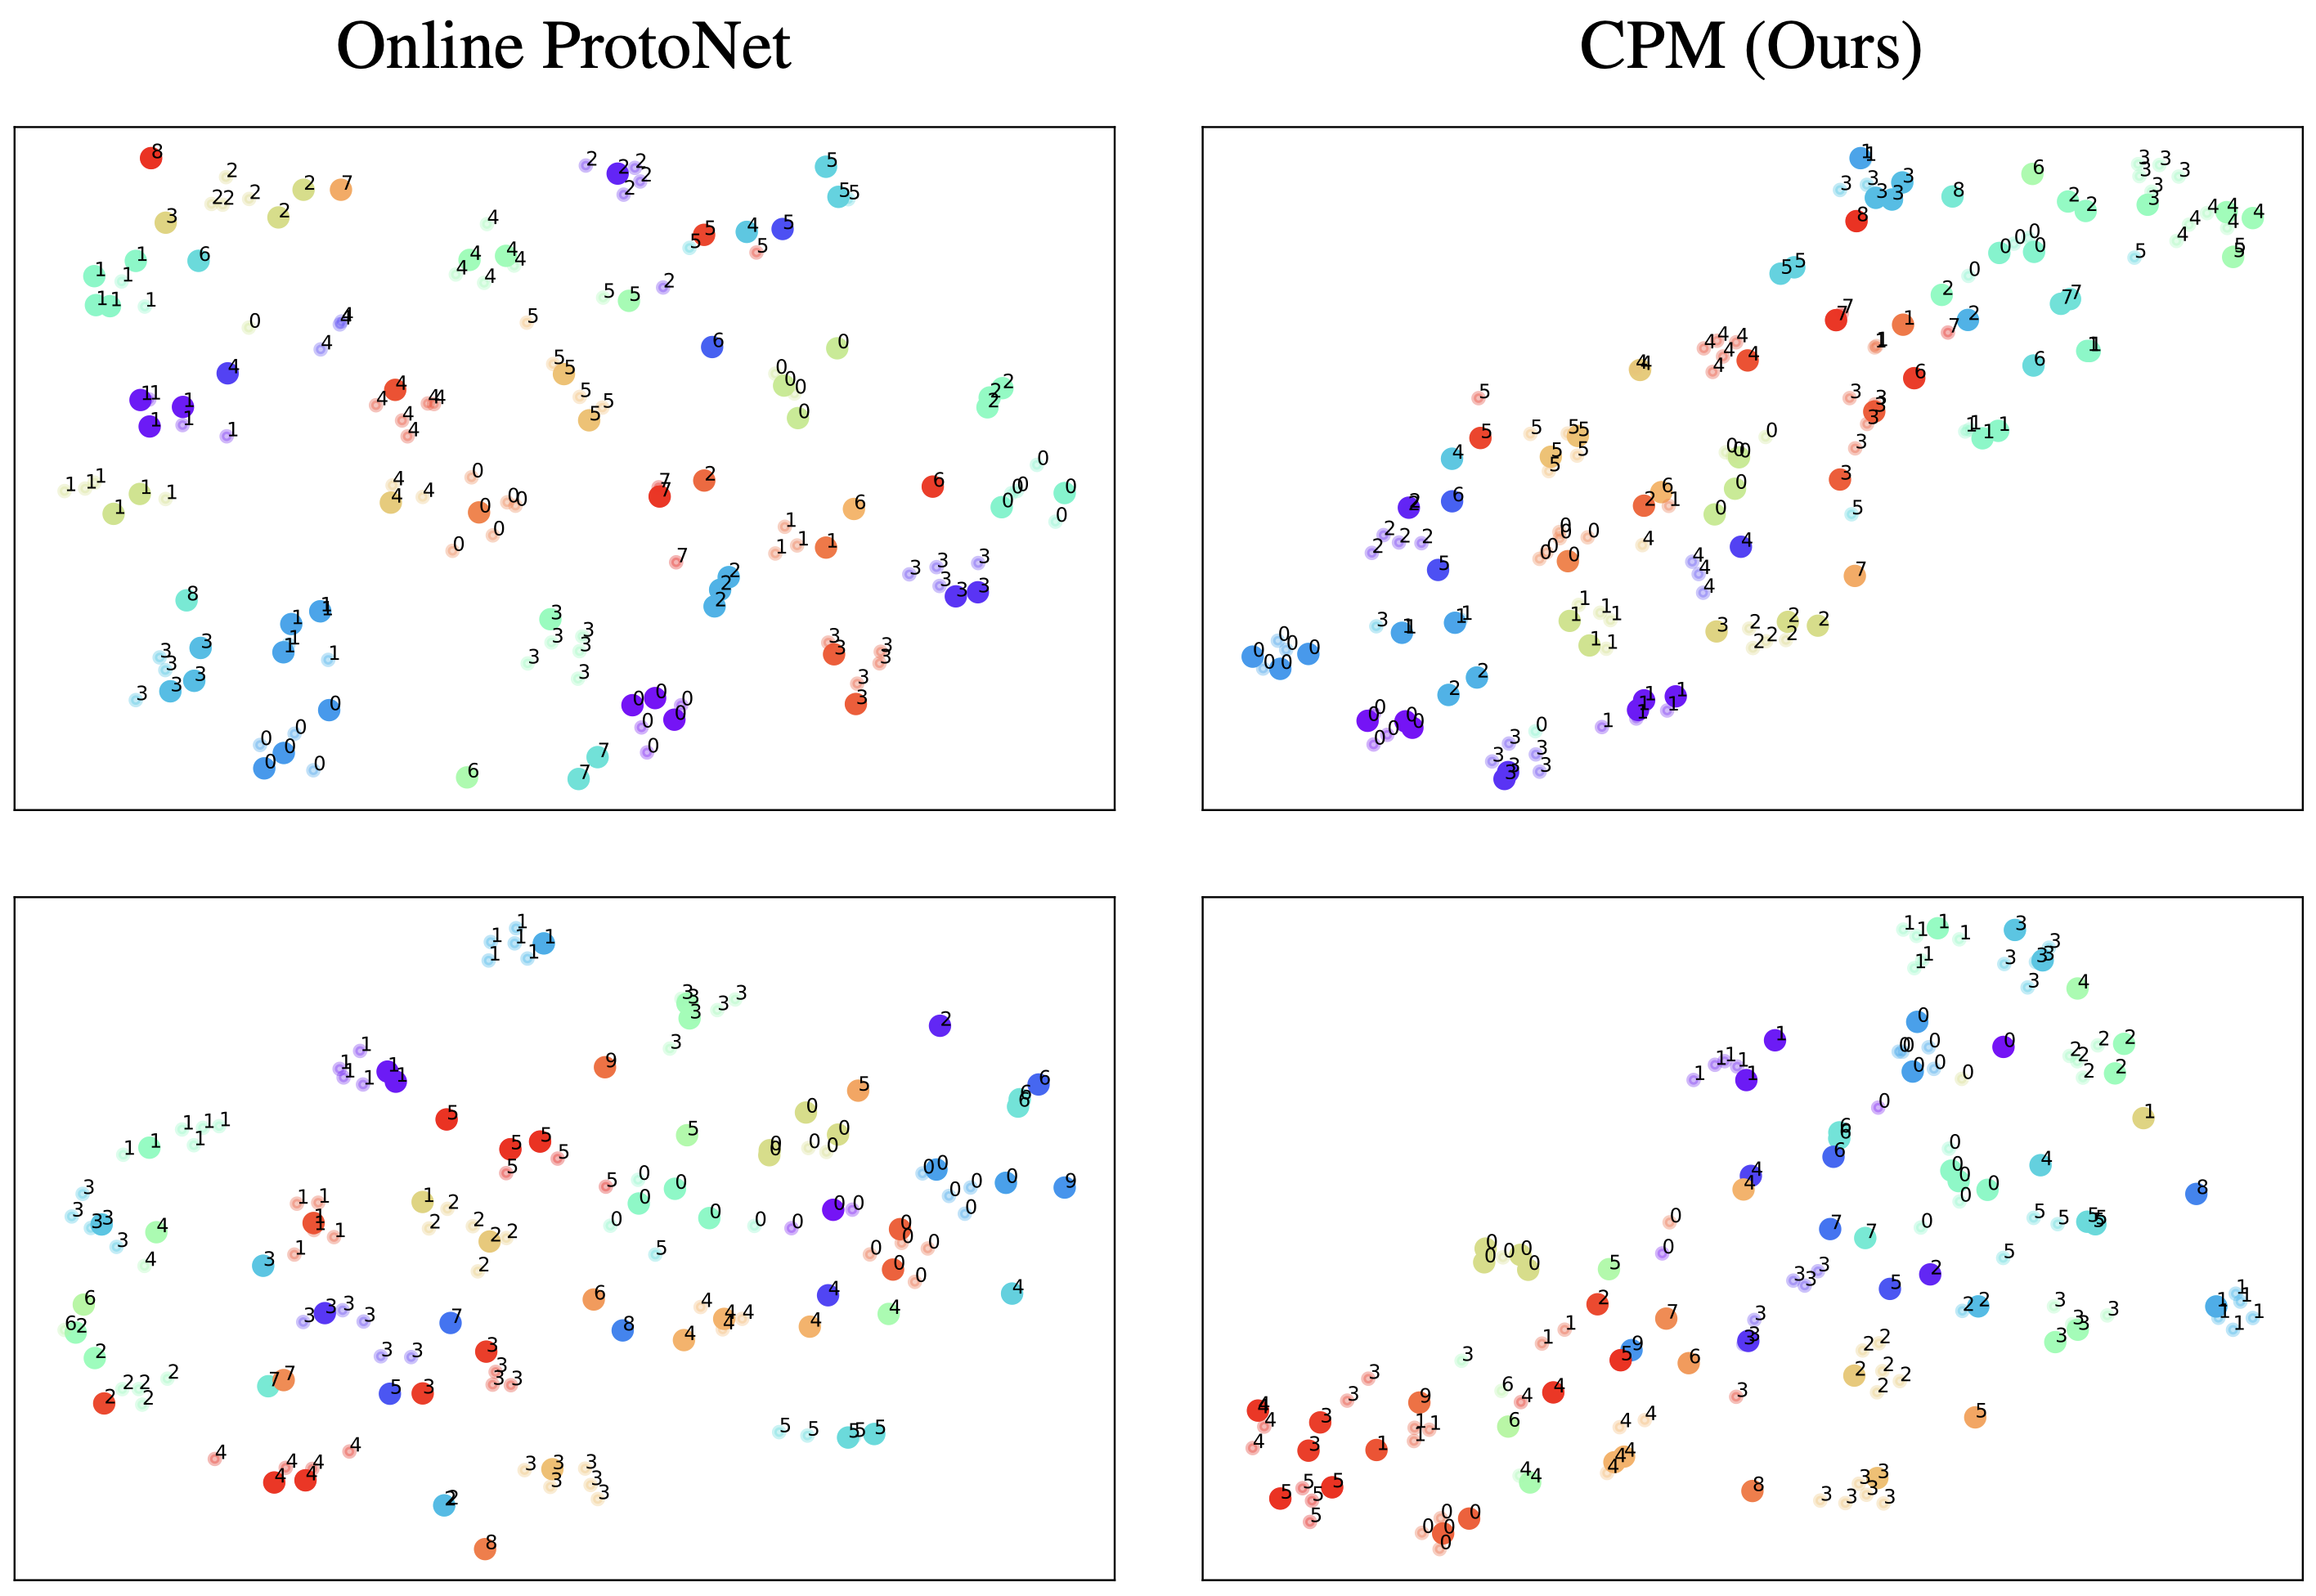
\includegraphics[width=6\linewidth]{figures/omniglot-tsne.png}
\else
    \begin{tabular}{cc}
    Online ProtoNet & CPM (Ours) \\
    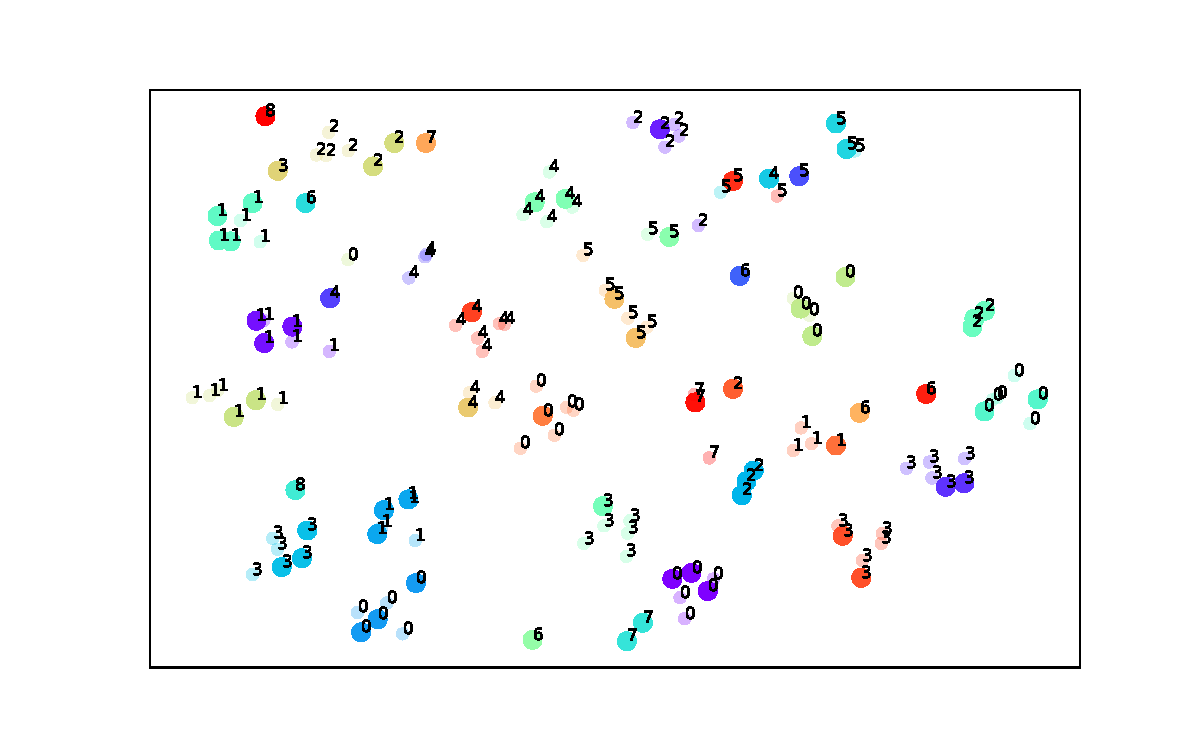
\includegraphics[height=3.8cm, trim={2.5cm 1cm 2cm 1cm}, clip]{figures/omniglot-protonet-tsne/tsne-003.pdf}
    &
    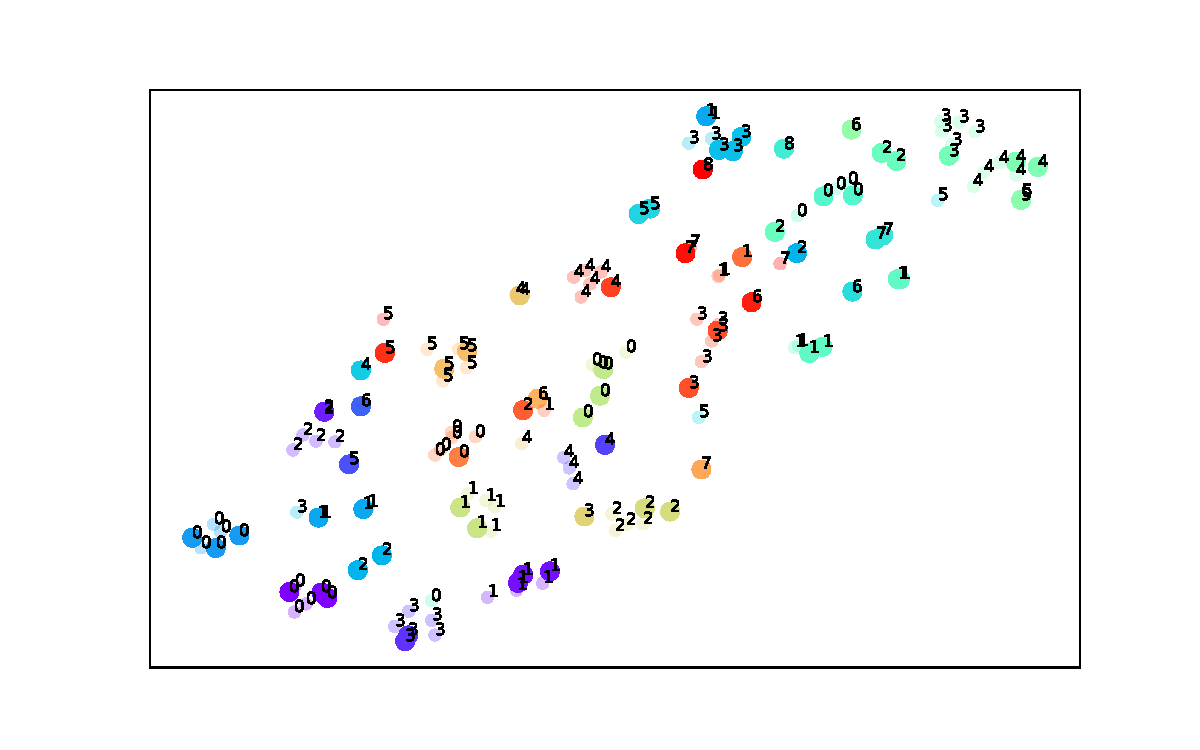
\includegraphics[height=3.8cm, trim={2.5cm 1cm 2cm 1cm}, clip]{figures/omniglot-cpm-tsne/tsne-003.pdf}
    \\
    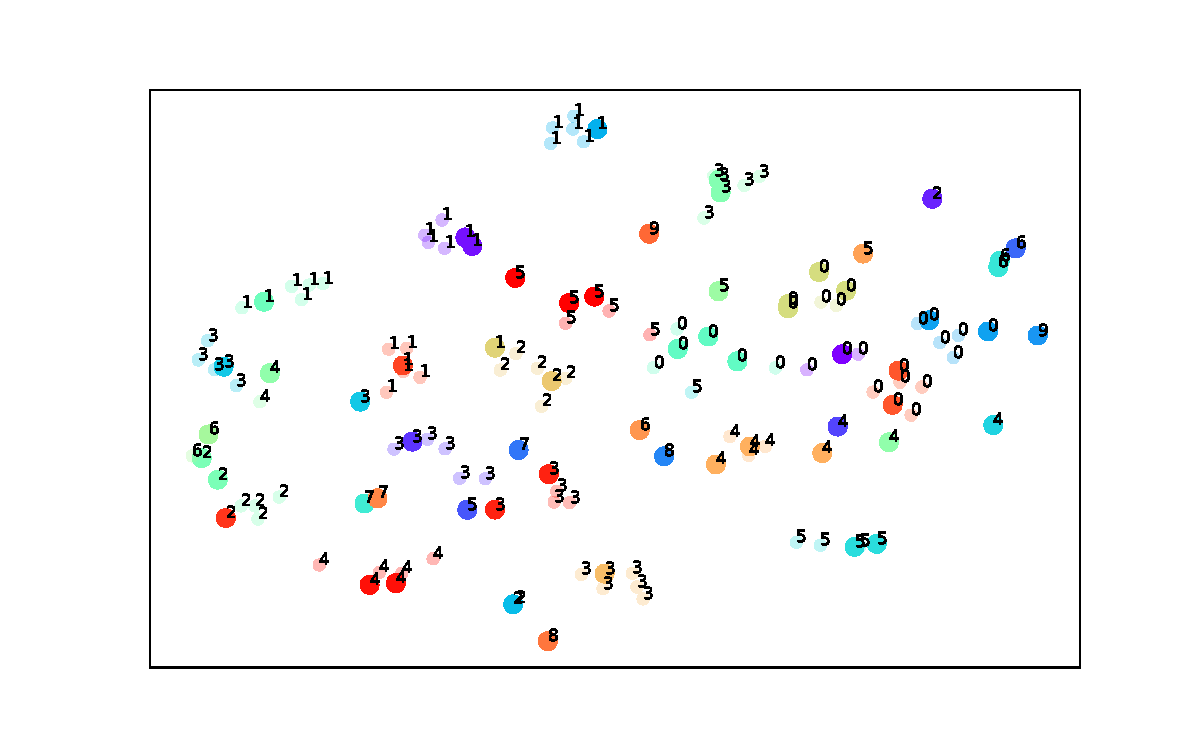
\includegraphics[height=3.8cm, trim={2.5cm 1cm 2cm 1cm}, clip]{figures/omniglot-protonet-tsne/tsne-008.pdf}
    &
    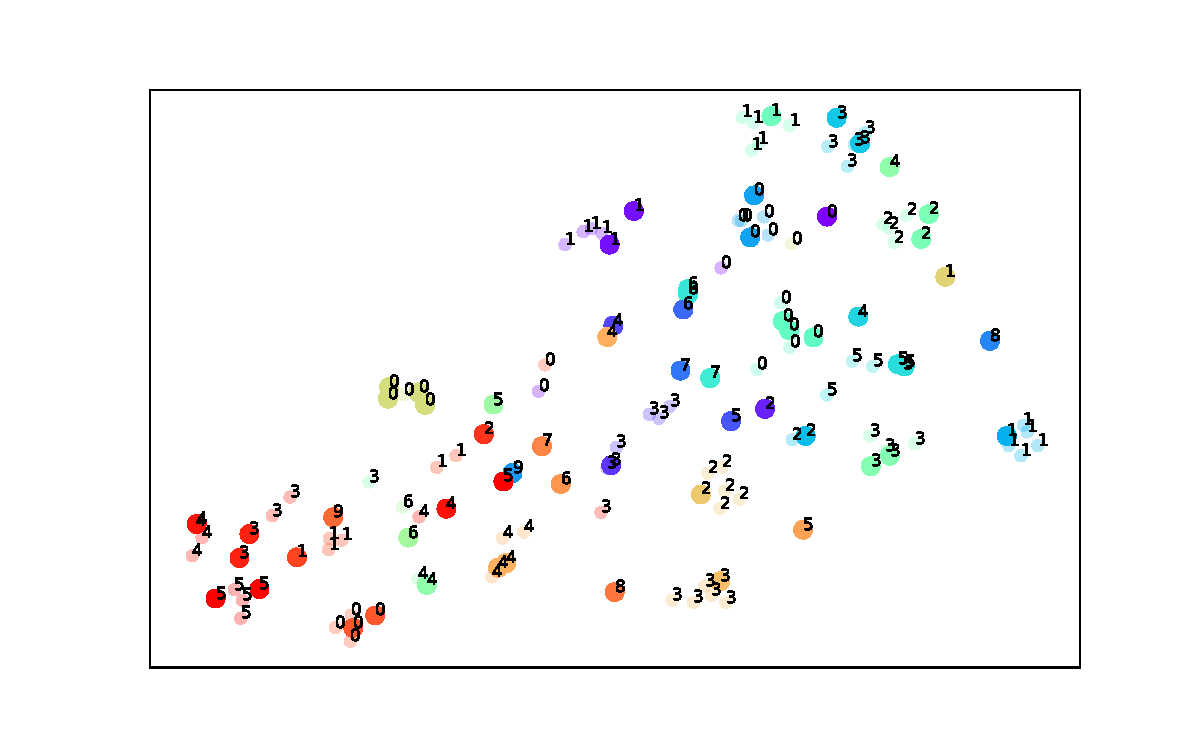
\includegraphics[height=3.8cm, trim={2.5cm 1cm 2cm 1cm}, clip]{figures/omniglot-cpm-tsne/tsne-008.pdf}
    \end{tabular}
\fi
\caption{\textbf{Embedding space visualization of \ourchar{} sequences using t-SNE~\citep{tsne}}. Different color
denotes different environments. Text labels (relative to each environment) are annotated beside the
scatter points. Unlabeled examples shown in smaller circles with lighter colors. \textbf{Left:}
Online ProtoNet; \textbf{Right:} CPM. The embeddings learned CPM model shows a smoother transition
of classes based on their temporal environments.}
\label{fig:tsne}
\end{figure}


% \paragraph{Control parameters vs. time:}
% Finally we visualize the control parameter values predicted by the RNN in
% Figure~\ref{fig:betagamma}. We verify that we indeed need two sets of $\beta$ and $\gamma$ for read
% and write operations separately as they learn different values. $\beta^w$ is smaller than $\beta^r$
% which means that the network is more conservative when writing to prototypes. $\gamma^w$ grows
% larger over time, which means that the network prefers a softer slope when writing
% to prototypes since in the later stage the prototype memory has already stored enough content and it can grow faster, whereas in the earlier stage, the prototype memory is more conservative to avoid embedding vectors to be assigned to wrong clusters.

% % !TEX root = ../supp.tex
\begin{figure}
\centering
% \vspace{-0.1in}
\iflatexml
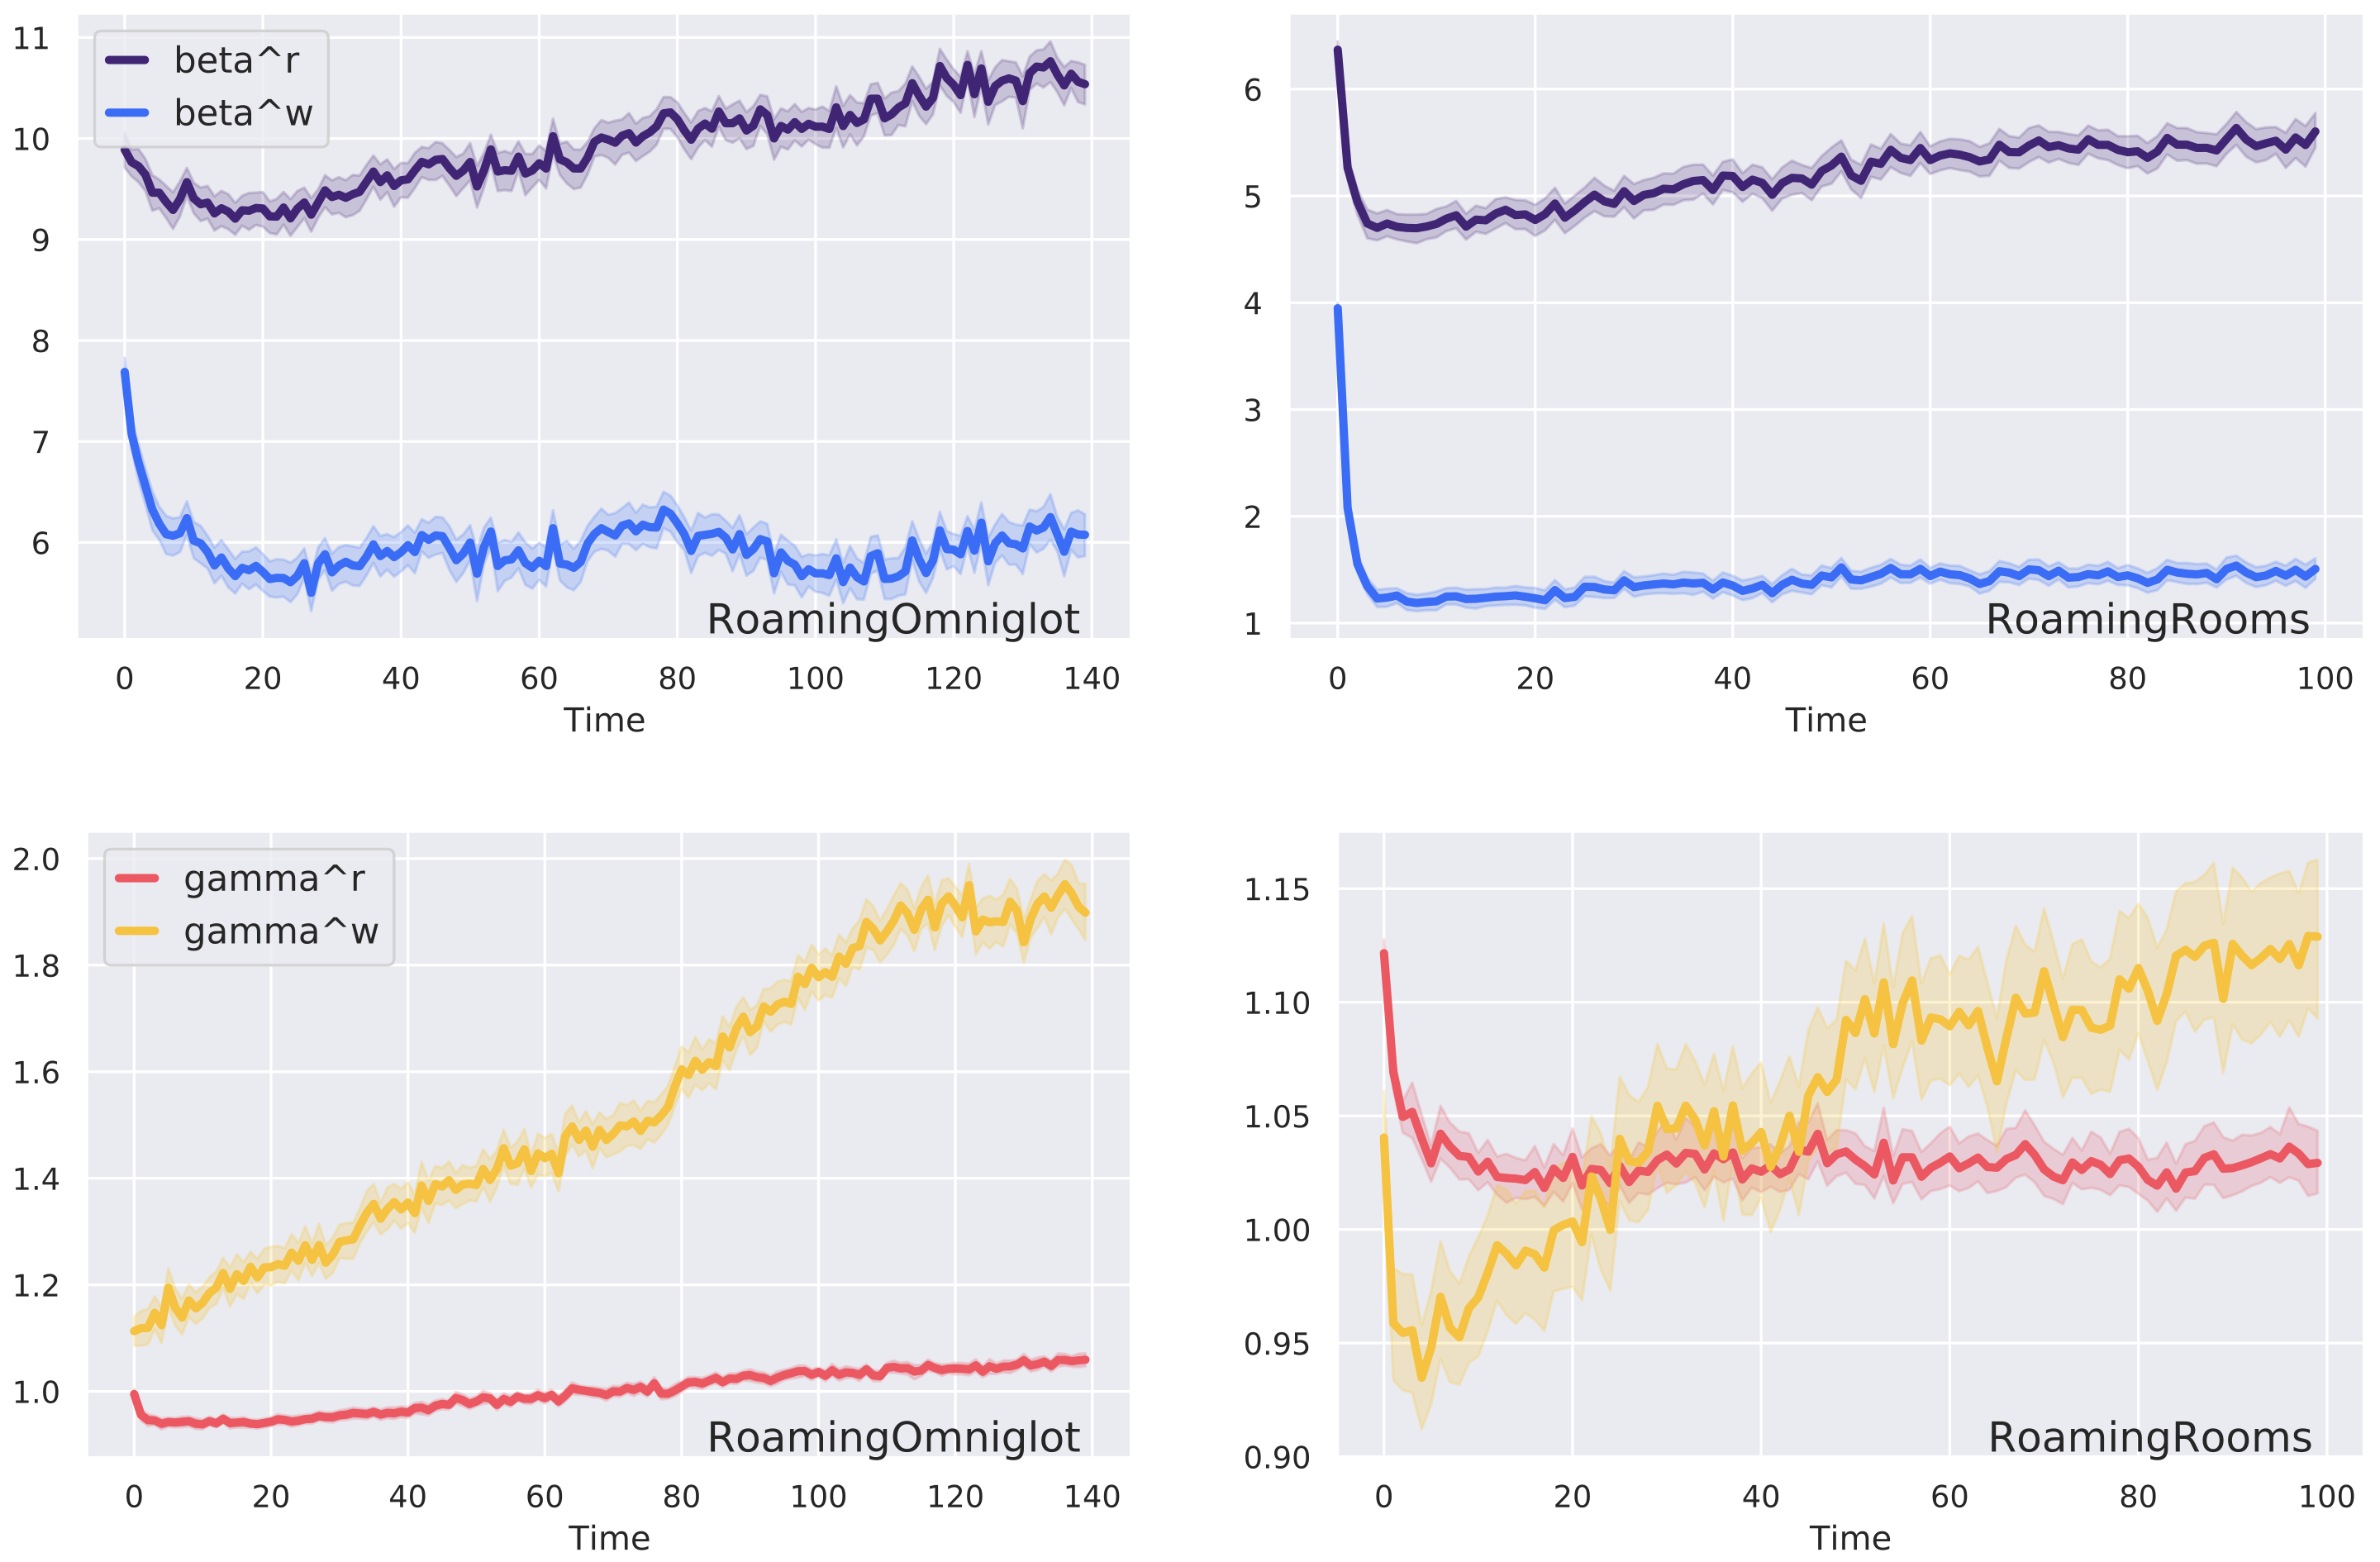
\includegraphics[width=6\linewidth]{figures/beta-gamma.png}
\else
\begin{tabular}{cc}
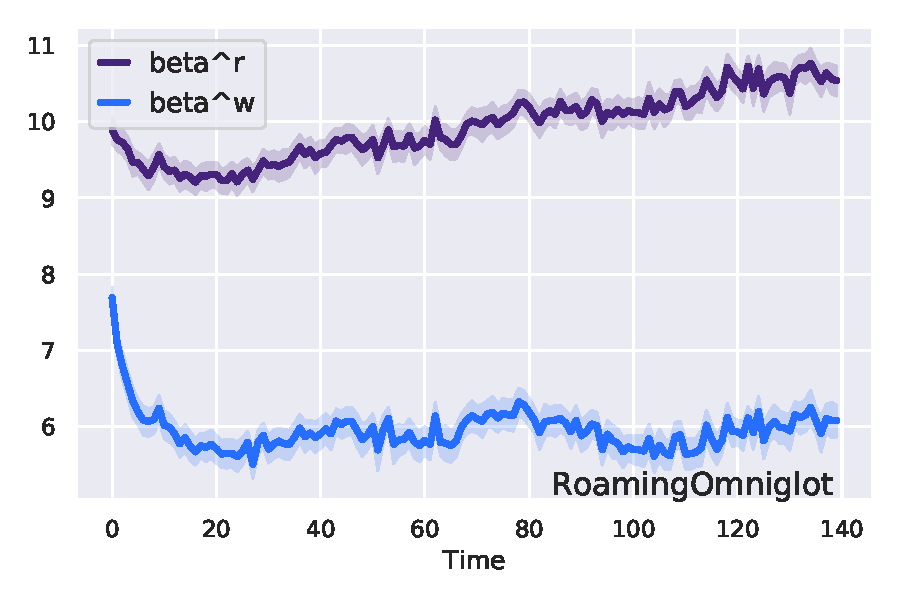
\includegraphics[height=4.0cm,trim={0.3cm 0cm 0.5cm 0},clip]{figures/omniglot-beta.pdf}
\quad
&
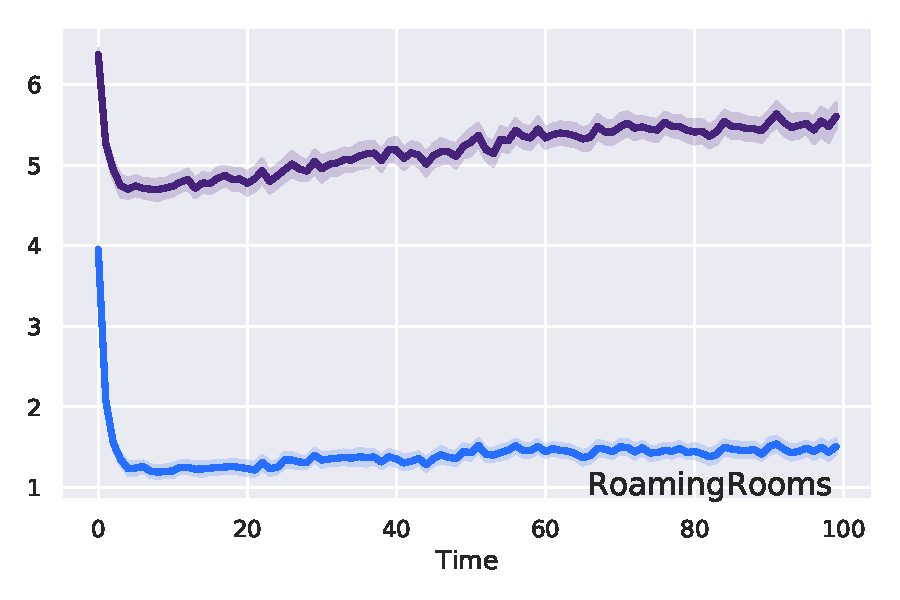
\includegraphics[height=4.0cm,trim={0.3cm 0cm 0cm 0},clip]{figures/matterport-beta.pdf}
\\
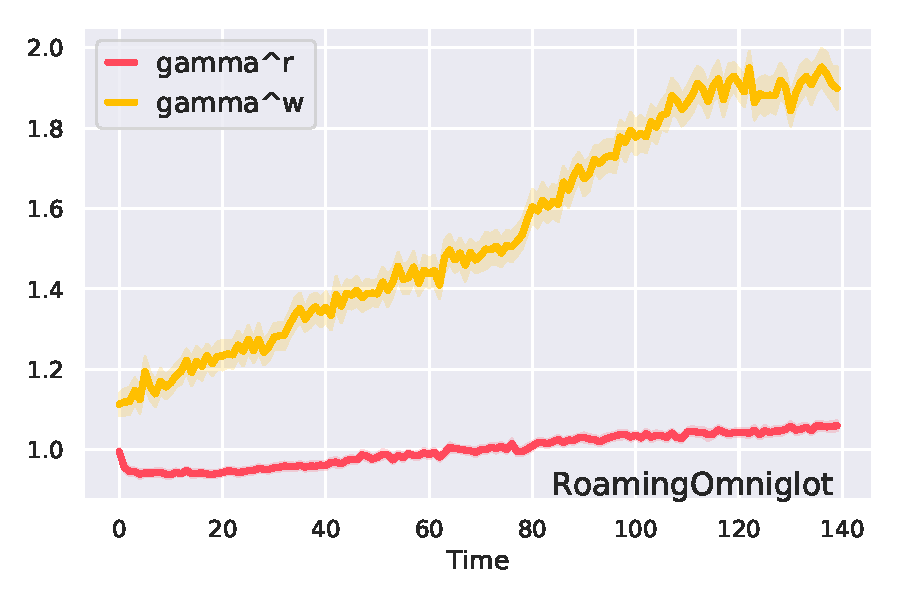
\includegraphics[height=4.0cm,trim={0.3cm 0cm 0.5cm 0},clip]{figures/omniglot-gamma.pdf}
\quad
&
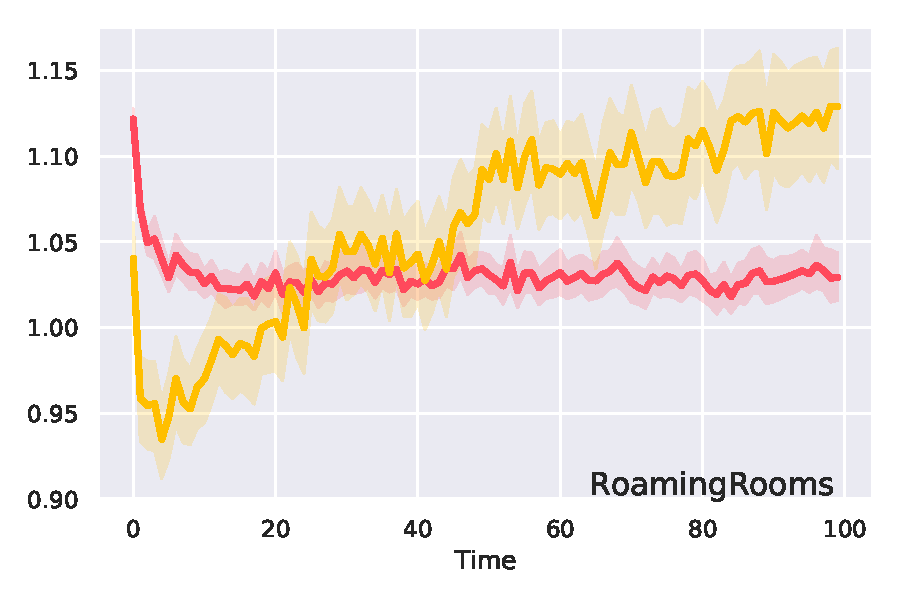
\includegraphics[height=4.0cm,trim={0.3cm 0cm 0cm 0},clip]{figures/matterport-gamma.pdf}
\\
\end{tabular}
\vspace{-0.1in}
\fi
\caption{\textbf{CPM control parameters ($\beta^{r,w}, \gamma^{r,w}$) vs. time.}
\textbf{Left:} \ourchar{} sequences; \textbf{Right:} \ourroom{} sequences; \textbf{Top:}
$\beta^{r,w}$ the threshold parameter; \textbf{Bottom:} $\gamma^{r,w}$ the temperature parameter.}
\label{fig:betagamma}
\end{figure}

% !TEX root = ../main.tex
\section{Dataset Details}
\label{app:data}

\subsection{Benchmark comparison}
We include Table~\ref{tab:benchmark} to compare existing continual and few-shot learning paradigms.

\subsection{\ourchar{} \& \ourimg{} Sampler Details}
For the \ourchar{} and the \ourimg{} experiments, we use sequences with maximum 150 images, from 5 environments. For
individual environment, we use a Chinese restaurant process to sample the class distribution. In
particular, the probability of sampling a new class is:
\begin{align}
p_\text{new} = \frac{k \alpha + \theta}{m + \theta},
\end{align}
where $k$ is the number of classes that we have already sampled in the environment, and $m$ is the
total number of instances we have in the environment. $\alpha$ is set to 0.2 and $\theta$ is set to
1.0 in all experiments.

The environment switching is implemented by a Markov switching process. At each step in the
sequence there is a constant probability $p_\text{switch}$ that switches to another environment. For
all experiments, we set $p_\text{switch}$ to 0.2. We truncate the maximum number of appearances
per class to 6. If the maximum appearance is reached, we will sample another class.

\subsection{Metrics}
\label{sec:metrics}
\paragraph{Average precision:} We chose to use AP (average precision or area under the precision-recall curve) as a way of integrating two aspects of performance:

\begin{enumerate}
    \item the binary accuracy of whether an instance belongs to a known or unknown class (KU-Assign for short), and
    \item the accuracy of assigning an instance the correct class label given it is from a known class (Class-Assign for short).
\end{enumerate}
The procedure to calculate AP is as follows. We first sort all the {KU-Assign, Class-Assign} predictions across all sequences in descending order based on KU-Assign probability, where the high ranked predictions should be known (not novel) classes. For the N top ranked instances in the sorted list, we compute:
\begin{enumerate}
    \item precision@N = correct(Class-Assign)@N / N
    \item recall@N = correct(Class-Assign)@N / K,
\end{enumerate}
where K is the true number of known instances and correct(Class-Assign)@N is the count of the number of correct class assignments among the top N. (The class assignment for an unknown instance is always incorrect.) To obtain the AP, we compute the integral of the function (y=precision@N, x=recall@N) across all N’s.

\paragraph{N-shot accuracy:} We define N-shot accuracy as the number of times an instance that has been seen N times thus far in the sequence is classified correctly. We compute the mean and standard error of this over all sequences.

\subsection{Additional \ourroom{} Statistics} 
Statistics of the \ourroom{} are included in Table~\ref{tab:dataset_stats}, in comparison to other
few-shot and continual learning datasets. Note that since \ourroom{} is collected from a simulated
environment, with 90 indoor worlds consisting of 1.2K panorama images and 1.22M video frames. The
dataset contains about 6.9K random walk sequences with a maximum of 200 frames per sequence. For
training we randomly crop 100 frames to form a training sequence. There are 7.0K unique instance
classes.

Plots of additional statistics of \ourroom{} are shown in Figure~\ref{fig:additionalstats}. In
addition to the ones shown in the main paper, instances and viewpoints also follow long tail
distributions. The number of objects in each frame follows an exponential distribution.

% !TEX root = ../main.tex
\begin{table}[t]
\iflatexml
    \begin{tabular}{ccccccc}
    \toprule
                                  & {\bf Images} & {\bf Sequences} & {\bf Classes} & {\bf Content}                  \\
    \midrule                                                                     
    Permuted MNIST~\citep{mnist}   & 60K          & -           & -          & Hand written digits          \\
    Omniglot~\citep{omniglot}      & 32.4K        & -           & 1.6K       & Hand written characters      \\
    CIFAR-100~\citep{cifar}        & 50K          & -           & 100        & Common objects               \\
    mini-ImageNet~\citep{matchingnet}& 50K        & -           & 100        & Common objects               \\
    tiered-ImageNet~\citep{fewshotssl}& 779K      & -           & 608        & Common objects               \\
    OpenLORIS  \citep{openloris}   & 98K          & -           & 69         & Small table-top obj.         \\
    CORe50  \citep{core50}         & 164.8K       & 11          & 50         & Hand-held obj.               \\
    \midrule                                                                                                          
    \ourroom{} (Ours)            & 1.22M         & 6.9K        & 7.0K       & General indoor instances     \\
    \bottomrule
    \end{tabular}
    \caption{\small Continual \& few-shot learning datasets}
    \label{tab:dataset_stats}
\else
    \vspace{-0.5in}
    \begin{center}
    \begin{small}
    \caption{\small Continual \& few-shot learning datasets}
    \label{tab:dataset_stats}
    \begin{tabular}{ccccccc}
    \toprule
                                  & {\bf Images} & {\bf Sequences} & {\bf Classes} & {\bf Content}                  \\
    \midrule                                                                     
    Permuted MNIST~\citep{mnist}   & 60K          & -           & -          & Hand written digits          \\
    Omniglot~\citep{omniglot}      & 32.4K        & -           & 1.6K       & Hand written characters      \\
    CIFAR-100~\citep{cifar}        & 50K          & -           & 100        & Common objects               \\
    mini-ImageNet~\citep{matchingnet}& 50K        & -           & 100        & Common objects               \\
    tiered-ImageNet~\citep{fewshotssl}& 779K      & -           & 608        & Common objects               \\
    OpenLORIS  \citep{openloris}   & 98K          & -           & 69         & Small table-top obj.         \\
    CORe50  \citep{core50}         & 164.8K       & 11          & 50         & Hand-held obj.               \\
    \midrule                                                                                                          
    \ourroom{} (Ours)            & 1.22M         & 6.9K        & 7.0K       & General indoor instances     \\
    \bottomrule
    \end{tabular}
    \vspace{-0.2in}
    \end{small}
    \end{center}
\fi
\end{table}


\subsection{\ourroom{} Simulator Details}
We generate our episodes with a two-stage process using two simulators -- HabitatSim~\citep{habitat}
and MatterSim~\citep{mattersim} -- because HabitatSim is based on 3D meshes and using HabitatSim
alone will result in poor image quality due to incorrect mesh reconstruction. Therefore we
sacrificed the continuous movement of agents within HabitatSim and base our environment navigation
on the discrete viewpoints in MatterSim, which is based on real panoramic images. The horizontal
field of view is set to 90 degrees for HabitatSim and 100 degrees for MatterSim, and we simulate
with\ 800$\times$600 resolution.

The first stage of generation involves randomly picking a sequence of viewpoints on the connectivity
graph within MatterSim. For each viewpoint, the agent scans the environment along the yaw and pitch
axes for a random period of time until a navigable viewpoint is within view. The time spent in a
single viewpoint follows a Gaussian distribution with mean 5.0 and standard deviation 1.0. At the
start of each new viewpoint, the agent randomly picks a direction to rotate and takes 12.5 degree
steps along the yaw axis, and with 95\% probability, a 5 degree rotation along the pitch axis is
applied in a randomly chosen direction. When a navigable viewpoint is detected, the agent will
navigate to the new viewpoint and reset the direction of scan. When multiple navigable viewpoints
are present, the agent uniformly samples one.

In the second stage, an agent in HabitatSim retraces the viewpoint path and movements of the first
stage generated by MatterSim, collecting mesh-rendered RGB and instance segmentation sensor data.
The MatterSim RGB and HabitatSim RGB images are then aligned via FLANN-based feature matching
~\citep{muja2009flann}, resulting in an alignment matrix that is used to place the MatterSim RGB and
HabitatSim instance segmentation maps into alignment. The sequence of these MatterSim RGB and
HabitatSim instance segmentation maps constitute an episode.

We keep objects of the following categories: \texttt{picture, chair, lighting, cushion, table,
plant, chest of drawers, towel, sofa, bed, appliances, stool, tv monitor, clothes, toilet,
fireplace, furniture, bathtub, gym equipment, blinds, board panel}. We initially generate 600 frames
per sequence and remove all the frames with no object. Then we store every 200 image frames into a
separate file.

During training and evaluation, each video sequence is loaded, and for each image we go through each
object present in the image. We create the attention map using the segmentation groundtruth of the
selected object. The attention map and the image together form a \textit{frame} in our model input.
For training, we randomly crop 100 frames from the sequence, and for evaluation we use the first 100
frames for deterministic results.

Please visit our released code repository to download the \ourroom{} dataset.

% !TEX root = ../main.tex
\begin{table*}[t]
\iflatexml
    \begin{tabular}{ccccccc}
    \toprule
    \mr{2}{\tb{Tasks}}                     & \tb{Few}  & \tb{Semi-sup. } & \mr{2}{\tb{Continual}} & \tb{Online} & \tb{Predict}& \tb{Soft Context}  \\
                                           & \tb{Shot} & \tb{Supp. Set}  &                        & \tb{Eval.}  & \tb{New}    & \tb{Switch}        \\
    \midrule                                                                                                                                                                          
    Incremental Learning (IL) \citep{icarl}& \xm       & \xm             & \cm                    & \hx         & \xm         & \xm                \\
    Few-shot (FSL) \citep{matchingnet}     & \cm       & \xm             & \xm                    & \xm         & \xm         & \xm                \\
    Incremental FSL \citep{attnattractor}  & \cm       & \xm             & \hx                    & \xm         & \xm         & \xm                \\
    Cls. Incremental FSL \citep{fscil}     & \cm       & \xm             & \cm                    & \hx         & \xm         & \xm                \\
    Semi-supv. FSL \citep{fewshotssl}      & \cm       & \cm             & \xm                    & \xm         & \cm         & \xm                \\
    MOCA \citep{moca}                      & \cm       & \xm             & \cm                    & \xm         & \xm         & \hx                \\
    Online Mixture \citep{onlinemixture}   & \cm       & \xm             & \cm                    & \xm         & \xm         & \hx                \\
    Online Meta \citep{oml}                & \cm       & \xm             & \cm                    & \xm         & \xm         & \xm                \\
    Continual FSL* \citep{contfsl}         & \cm       & \xm             & \cm                    & \xm         & \xm         & \xm                \\
    OSAKA* \citep{osaka}                   & \cm       & \xm             & \cm                    & \cm         & \hx         & \cm                \\
    \midrule                                                                                                                                                                                         
    OC-FSL (Ours)                          & \cm       & \cm             & \cm                    & \cm         & \cm         & \cm                \\
    \bottomrule
    \end{tabular}
    \caption{Comparison of past FSL and CL paradigms vs. our online contextualized FSL (OC-FSL). * denotes concurrent work.}
    \label{tab:benchmark}
\else
    \vspace{-0.5in}
    \caption{Comparison of past FSL and CL paradigms vs. our online contextualized FSL (OC-FSL).}
    \begin{center}
    \begin{small}
    \resizebox{\textwidth}{!}{
    \begin{tabular}{ccccccc}
    \toprule
    \mr{2}{\tb{Tasks}}                     & \tb{Few}  & \tb{Semi-sup. } & \mr{2}{\tb{Continual}} & \tb{Online} & \tb{Predict}& \tb{Soft Context}  \\
                                           & \tb{Shot} & \tb{Supp. Set}  &                        & \tb{Eval.}  & \tb{New}    & \tb{Switch}        \\
    \midrule                                                                                                                                                                          
    Incremental Learning (IL) \citep{icarl}& \xm       & \xm             & \cm                    & \hx         & \xm         & \xm                \\
    Few-shot (FSL) \citep{matchingnet}     & \cm       & \xm             & \xm                    & \xm         & \xm         & \xm                \\
    Incremental FSL \citep{attnattractor}  & \cm       & \xm             & \hx                    & \xm         & \xm         & \xm                \\
    Cls. Incremental FSL \citep{fscil}     & \cm       & \xm             & \cm                    & \hx         & \xm         & \xm                \\
    Semi-supv. FSL \citep{fewshotssl}      & \cm       & \cm             & \xm                    & \xm         & \cm         & \xm                \\
    MOCA \citep{moca}                      & \cm       & \xm             & \cm                    & \xm         & \xm         & \hx                \\
    Online Mixture \citep{onlinemixture}   & \cm       & \xm             & \cm                    & \xm         & \xm         & \hx                \\
    Online Meta \citep{oml}                & \cm       & \xm             & \cm                    & \xm         & \xm         & \xm                \\
    Continual FSL* \citep{contfsl}         & \cm       & \xm             & \cm                    & \xm         & \xm         & \xm                \\
    OSAKA* \citep{osaka}                   & \cm       & \xm             & \cm                    & \cm         & \hx         & \cm                \\
    \midrule                                                                                                                                                                                         
    OC-FSL (Ours)                          & \cm       & \cm             & \cm                    & \cm         & \cm         & \cm                \\
    \bottomrule
    \end{tabular}
    }
    \label{tab:benchmark}
    \\
    \vspace{0.05in}
    * denotes concurrent work.
    \end{small}
    \end{center}
\fi
\end{table*}

\subsection{Semi-supervised Labels:}
Here we describe how we sample the labeled vs. unlabeled flag for each example in the
semi-supervised sequences in both \ourchar{} and \ourroom{} datasets. Due to the imbalance in our
class distribution (from both the Chinese restaurant process and real data collection), directly
masking the label may bias the model to ignore the rare seen classes. Ideally, we would like to
preserve at least one labeled example for each class. Therefore, we designed the following
procedure.

First, for each class $k$, suppose $m_k$ is the number of examples in the sequence that belong to
the class. Let $\alpha$ be the target label ratio. Then the class-specific label ratio $\alpha_k$
is:
\begin{align}
\alpha_k = (1 - \alpha) \exp(-0.5 (m_k - 1)) + \alpha.
\label{eq:semisup}
\end{align}
We then for each class $k$, we sample a binary Bernoulli sequence based on $\Ber(\alpha_k)$. If a
class has all zeros in the Bernoulli sequence, we flip the flag of one of the instances to 1 to make
sure there is at least one labeled instance for each class.
For all experiments, we set $\alpha = 0.3$.

\subsection{Dataset Splits}
We include details about our dataset splits in Table~\ref{tab:omniglotsplit} and
\ref{tab:matterportsplit}.

\section{Experiment Details}
\label{app:exp}
\subsection{Network Architecture}
For the \ourchar{} experiment we used the common 4-layer CNN for few-shot learning with 64 channels
in each layer, resulting in a 64-d feature vector~\citep{protonet}. For the \ourroom{} experiment we
resize the input to 120$\times$160 and we use the ResNet-12 architecture~\citep{tadam} with
\{32,64,128,256\} channels per block. To represent the feature of the input image with an attention
mask, we concatenate the global average pooled feature with the attention ROI feature, resulting in
a 512d feature vector. For the contextual RNN, in both experiments we used an LSTM~\citep{lstm} with
a 256d hidden state. 

We use a linear layer to map from the output of the RNN to the features and control variables. We
obtain $\gamma^{r,w}$ by adding 1.0 to the linear layer output and then applying the softplus
activation. The bias units for $\beta^{r,w}$ are initialized to 10.0. We
also apply the softplus activation to $\bmm$ from the linear layer output.

% !TEX root = ../main.tex
\begin{table}[t]
\iflatexml
    \begin{tabular}{clll}
    \toprule

    \mr{11}{Train} &
    \texttt{Angelic} &
    \texttt{Grantha} &
    \texttt{N Ko}\\
    & 
    \texttt{Aurek-Besh} &
    \texttt{Japanese (hiragana)} &
    \texttt{Malay}
    \\
    & 
    \texttt{Asomtavruli} &
    \texttt{Sanskrit} &
    \texttt{Ojibwe}
    \\
    & 
    \texttt{Korean} &
    \texttt{Arcadian} &
    \texttt{Greek}
    \\
    & 
    \texttt{Alphabet of the Magi} &
    \texttt{Blackfoot} &
    \texttt{Futurama}
    \\
    & 
    \texttt{Tagalog} &
    \texttt{Anglo-Saxon Futhorc} &
    \texttt{Braille}
    \\
    & 
    \texttt{Cyrillic} &
    \texttt{Burmese} &
    \texttt{Avesta}
    \\
    & 
    \texttt{Gujarati} &
    \texttt{Ge ez} &
    \texttt{Syriac (Estrangelo)}
    \\
    & 
    \texttt{Atlantean} &
    \texttt{Japanese (katakana)} &
    \texttt{Balinese}
    \\
    & 
    \texttt{Atemayar Qelisayer} &
    \texttt{Glagolitic} &
    \texttt{Tifinagh}
    \\
    & 
    \texttt{Latin} &
    \texttt{Inuktitut} &
    \\
    \midrule
    \mr{2}{Val} &
    \texttt{Hebrew} &
    \texttt{Mkhedruli} &
    \texttt{Armenian}\\
    & 
    \texttt{Early Aramaic} &
    \texttt{Bengali} &
    \\
    \midrule

    \mr{5}{Test} & 
    \texttt{Gurmukhi} &
    \texttt{Kannada} & 
    \texttt{Keble} \\
    &
    \texttt{Malayalam} &
    \texttt{Manipuri} &
    \texttt{Mongolian} 
    \\
    &
    \texttt{Old Church Slavonic} &
    \texttt{Oriya} &
    \texttt{Syriac (Serto)} \\
    &
    \texttt{Sylheti} &
    \texttt{Tengwar} &
    \texttt{Tibetan}\\
    &
    \texttt{ULOG}
    \\
    \bottomrule
    \end{tabular}
     \caption{\textbf{Split information for {\it \ourchar{}}}. Each column is an alphabet and we include all the characters in the alphabet in the split. Rows are continuation of lines.}
    \label{tab:omniglotsplit}
\else
    \vspace{-0.5in}
     \caption{\textbf{Split information for {\it \ourchar{}}}. Each column is an alphabet and we include all the characters in the alphabet in the split. Rows are continuation of lines.}
    \begin{center}
    \begin{small}
    \label{tab:omniglotsplit}
    \begin{tabular}{clll}
    \toprule

    \mr{11}{Train} &
    \texttt{Angelic} &
    \texttt{Grantha} &
    \texttt{N Ko}\\
    & 
    \texttt{Aurek-Besh} &
    \texttt{Japanese (hiragana)} &
    \texttt{Malay}
    \\
    & 
    \texttt{Asomtavruli} &
    \texttt{Sanskrit} &
    \texttt{Ojibwe}
    \\
    & 
    \texttt{Korean} &
    \texttt{Arcadian} &
    \texttt{Greek}
    \\
    & 
    \texttt{Alphabet of the Magi} &
    \texttt{Blackfoot} &
    \texttt{Futurama}
    \\
    & 
    \texttt{Tagalog} &
    \texttt{Anglo-Saxon Futhorc} &
    \texttt{Braille}
    \\
    & 
    \texttt{Cyrillic} &
    \texttt{Burmese} &
    \texttt{Avesta}
    \\
    & 
    \texttt{Gujarati} &
    \texttt{Ge ez} &
    \texttt{Syriac (Estrangelo)}
    \\
    & 
    \texttt{Atlantean} &
    \texttt{Japanese (katakana)} &
    \texttt{Balinese}
    \\
    & 
    \texttt{Atemayar Qelisayer} &
    \texttt{Glagolitic} &
    \texttt{Tifinagh}
    \\
    & 
    \texttt{Latin} &
    \texttt{Inuktitut} &
    \\
    \midrule
    \mr{2}{Val} &
    \texttt{Hebrew} &
    \texttt{Mkhedruli} &
    \texttt{Armenian}\\
    & 
    \texttt{Early Aramaic} &
    \texttt{Bengali} &
    \\
    \midrule

    \mr{5}{Test} & 
    \texttt{Gurmukhi} &
    \texttt{Kannada} & 
    \texttt{Keble} \\
    &
    \texttt{Malayalam} &
    \texttt{Manipuri} &
    \texttt{Mongolian} 
    \\
    &
    \texttt{Old Church Slavonic} &
    \texttt{Oriya} &
    \texttt{Syriac (Serto)} \\
    &
    \texttt{Sylheti} &
    \texttt{Tengwar} &
    \texttt{Tibetan}\\
    &
    \texttt{ULOG}
    \\
    \bottomrule
    \end{tabular}
    \end{small}
    \end{center}
\fi
\end{table}

% !TEX root = ../main.tex
\iflatexml
\begin{table}[t]
\begin{tabular}{cc}
\toprule
\mr{12}{Train} &
\texttt{
r1Q1Z4BcV1o
JmbYfDe2QKZ
29hnd4uzFmX
ULsKaCPVFJR
E9uDoFAP3SH
}\\
&
\texttt{
8WUmhLawc2A
Uxmj2M2itWa
mJXqzFtmKg4
V2XKFyX4ASd
EU6Fwq7SyZv
}\\
&
\texttt{
gYvKGZ5eRqb
gxdoqLR6rwA
YFuZgdQ5vWj
gTV8FGcVJC9
sT4fr6TAbpF
}\\
&
\texttt{
VVfe2KiqLaN
fzynW3qQPVF
WYY7iVyf5p8
VFuaQ6m2Qom
YmJkqBEsHnH
}\\
&
\texttt{
2t7WUuJeko7
pLe4wQe7qrG
cV4RVeZvu5T
XcA2TqTSSAj
ur6pFq6Qu1A
}\\
&
\texttt{
1pXnuDYAj8r
b8cTxDM8gDG
x8F5xyUWy9e
X7HyMhZNoso
aayBHfsNo7d
}\\
&
\texttt{
TbHJrupSAjP
sKLMLpTHeUy
2azQ1b91cZZ
2n8kARJN3HM
Vvot9Ly1tCj
}\\
&
\texttt{
S9hNv5qa7GM
EDJbREhghzL
qoiz87JEwZ2
q9vSo1VnCiC
Vt2qJdWjCF2
}\\
&
\texttt{
VzqfbhrpDEA
D7G3Y4RVNrH
ZMojNkEp431
uNb9QFRL6hY
5LpN3gDmAk7
}\\
&
\texttt{
rqfALeAoiTq
e9zR4mvMWw7
yqstnuAEVhm
zsNo4HB9uLZ
JF19kD82Mey
}\\
&
\texttt{
759xd9YjKW5
wc2JMjhGNzB
rPc6DW4iMge
jh4fc5c5qoQ
HxpKQynjfin
}\\
&
\texttt{
GdvgFV5R1Z5
kEZ7cmS4wCh
vyrNrziPKCB
D7N2EKCX4Sj
PX4nDJXEHrG
}\\

\midrule

\mr{2}{Val} &
\texttt{
s8pcmisQ38h
dhjEzFoUFzH
RPmz2sHmrrY
1LXtFkjw3qL
8194nk5LbLH
}\\
&
\texttt{
jtcxE69GiFV
QUCTc6BB5sX
p5wJjkQkbXX
JeFG25nYj2p
82sE5b5pLXE
}\\
\midrule

\mr{4}{Test} & 
\texttt{
oLBMNvg9in8
r47D5H71a5s
Z6MFQCViBuw
YVUC4YcDtcY
pRbA3pwrgk9
}\\
&
\texttt{
SN83YJsR3w2
gZ6f7yhEvPG
ac26ZMwG7aT
7y3sRwLe3Va
B6ByNegPMKs
}\\
&
\texttt{
UwV83HsGsw3
VLzqgDo317F
17DRP5sb8fy
pa4otMbVnkk
5ZKStnWn8Zo
}\\
&
\texttt{
PuKPg4mmafe
Pm6F8kyY3z2
i5noydFURQK
ARNzJeq3xxb
5q7pvUzZiYa
}\\
\bottomrule
\end{tabular}
\caption{\textbf{Split information for {\it \ourroom{}}}. Each column is the ID of an indoor world. Rows are continuation of the lines.}
\label{tab:matterportsplit}
\end{table}

\begin{table}[t]
\begin{tabular}{cccc}
\toprule
Split & Worlds & Sequences & Frames \\
\midrule
Train & 60     & 4,699      &   823,444     \\
Val   & 20     &  725         &  125,823  \\
Test  & 10     &  1,547      &  271,335      \\
\midrule
Total & 90     & 6,971   & 1,220,602 \\
\bottomrule
\end{tabular}
\caption{{\it \ourroom{}} dataset split size}
\label{tab:matterportsplitsize}
\end{table}
\else
    \begin{table}[t]
    \caption{\textbf{Split information for {\it \ourroom{}}}. Each column is the ID of an indoor world. Rows are continuation of the lines.}
    \label{tab:matterportsplit}
    % \vspace{-0.5in}
    \begin{center}
    \begin{small}
    \begin{tabular}{cc}
    \toprule
    \mr{12}{Train} &
    \texttt{
    r1Q1Z4BcV1o
    JmbYfDe2QKZ
    29hnd4uzFmX
    ULsKaCPVFJR
    E9uDoFAP3SH
    }\\
    &
    \texttt{
    8WUmhLawc2A
    Uxmj2M2itWa
    mJXqzFtmKg4
    V2XKFyX4ASd
    EU6Fwq7SyZv
    }\\
    &
    \texttt{
    gYvKGZ5eRqb
    gxdoqLR6rwA
    YFuZgdQ5vWj
    gTV8FGcVJC9
    sT4fr6TAbpF
    }\\
    &
    \texttt{
    VVfe2KiqLaN
    fzynW3qQPVF
    WYY7iVyf5p8
    VFuaQ6m2Qom
    YmJkqBEsHnH
    }\\
    &
    \texttt{
    2t7WUuJeko7
    pLe4wQe7qrG
    cV4RVeZvu5T
    XcA2TqTSSAj
    ur6pFq6Qu1A
    }\\
    &
    \texttt{
    1pXnuDYAj8r
    b8cTxDM8gDG
    x8F5xyUWy9e
    X7HyMhZNoso
    aayBHfsNo7d
    }\\
    &
    \texttt{
    TbHJrupSAjP
    sKLMLpTHeUy
    2azQ1b91cZZ
    2n8kARJN3HM
    Vvot9Ly1tCj
    }\\
    &
    \texttt{
    S9hNv5qa7GM
    EDJbREhghzL
    qoiz87JEwZ2
    q9vSo1VnCiC
    Vt2qJdWjCF2
    }\\
    &
    \texttt{
    VzqfbhrpDEA
    D7G3Y4RVNrH
    ZMojNkEp431
    uNb9QFRL6hY
    5LpN3gDmAk7
    }\\
    &
    \texttt{
    rqfALeAoiTq
    e9zR4mvMWw7
    yqstnuAEVhm
    zsNo4HB9uLZ
    JF19kD82Mey
    }\\
    &
    \texttt{
    759xd9YjKW5
    wc2JMjhGNzB
    rPc6DW4iMge
    jh4fc5c5qoQ
    HxpKQynjfin
    }\\
    &
    \texttt{
    GdvgFV5R1Z5
    kEZ7cmS4wCh
    vyrNrziPKCB
    D7N2EKCX4Sj
    PX4nDJXEHrG
    }\\

    \midrule

    \mr{2}{Val} &
    \texttt{
    s8pcmisQ38h
    dhjEzFoUFzH
    RPmz2sHmrrY
    1LXtFkjw3qL
    8194nk5LbLH
    }\\
    &
    \texttt{
    jtcxE69GiFV
    QUCTc6BB5sX
    p5wJjkQkbXX
    JeFG25nYj2p
    82sE5b5pLXE
    }\\
    \midrule

    \mr{4}{Test} & 
    \texttt{
    oLBMNvg9in8
    r47D5H71a5s
    Z6MFQCViBuw
    YVUC4YcDtcY
    pRbA3pwrgk9
    }\\
    &
    \texttt{
    SN83YJsR3w2
    gZ6f7yhEvPG
    ac26ZMwG7aT
    7y3sRwLe3Va
    B6ByNegPMKs
    }\\
    &
    \texttt{
    UwV83HsGsw3
    VLzqgDo317F
    17DRP5sb8fy
    pa4otMbVnkk
    5ZKStnWn8Zo
    }\\
    &
    \texttt{
    PuKPg4mmafe
    Pm6F8kyY3z2
    i5noydFURQK
    ARNzJeq3xxb
    5q7pvUzZiYa
    }\\
    \bottomrule
    \end{tabular}
    \end{small}
    \end{center}
    \end{table}

    \begin{table}[t]
    \vspace{-0.5in}
    \caption{{\it \ourroom{}} dataset split size}
    \label{tab:matterportsplitsize}
    \begin{center}
    \begin{small}
    \begin{tabular}{cccc}
    \toprule
    Split & Worlds & Sequences & Frames \\
    \midrule
    Train & 60     & 4,699      &   823,444     \\
    Val   & 20     &  725         &  125,823  \\
    Test  & 10     &  1,547      &  271,335      \\
    \midrule
    Total & 90     & 6,971   & 1,220,602 \\
    \bottomrule
    \end{tabular}
    \end{small}
    \end{center}
    \end{table}
\fi


\begin{figure}[t]
\vspace{-0.2in}
\centering
\iflatexml
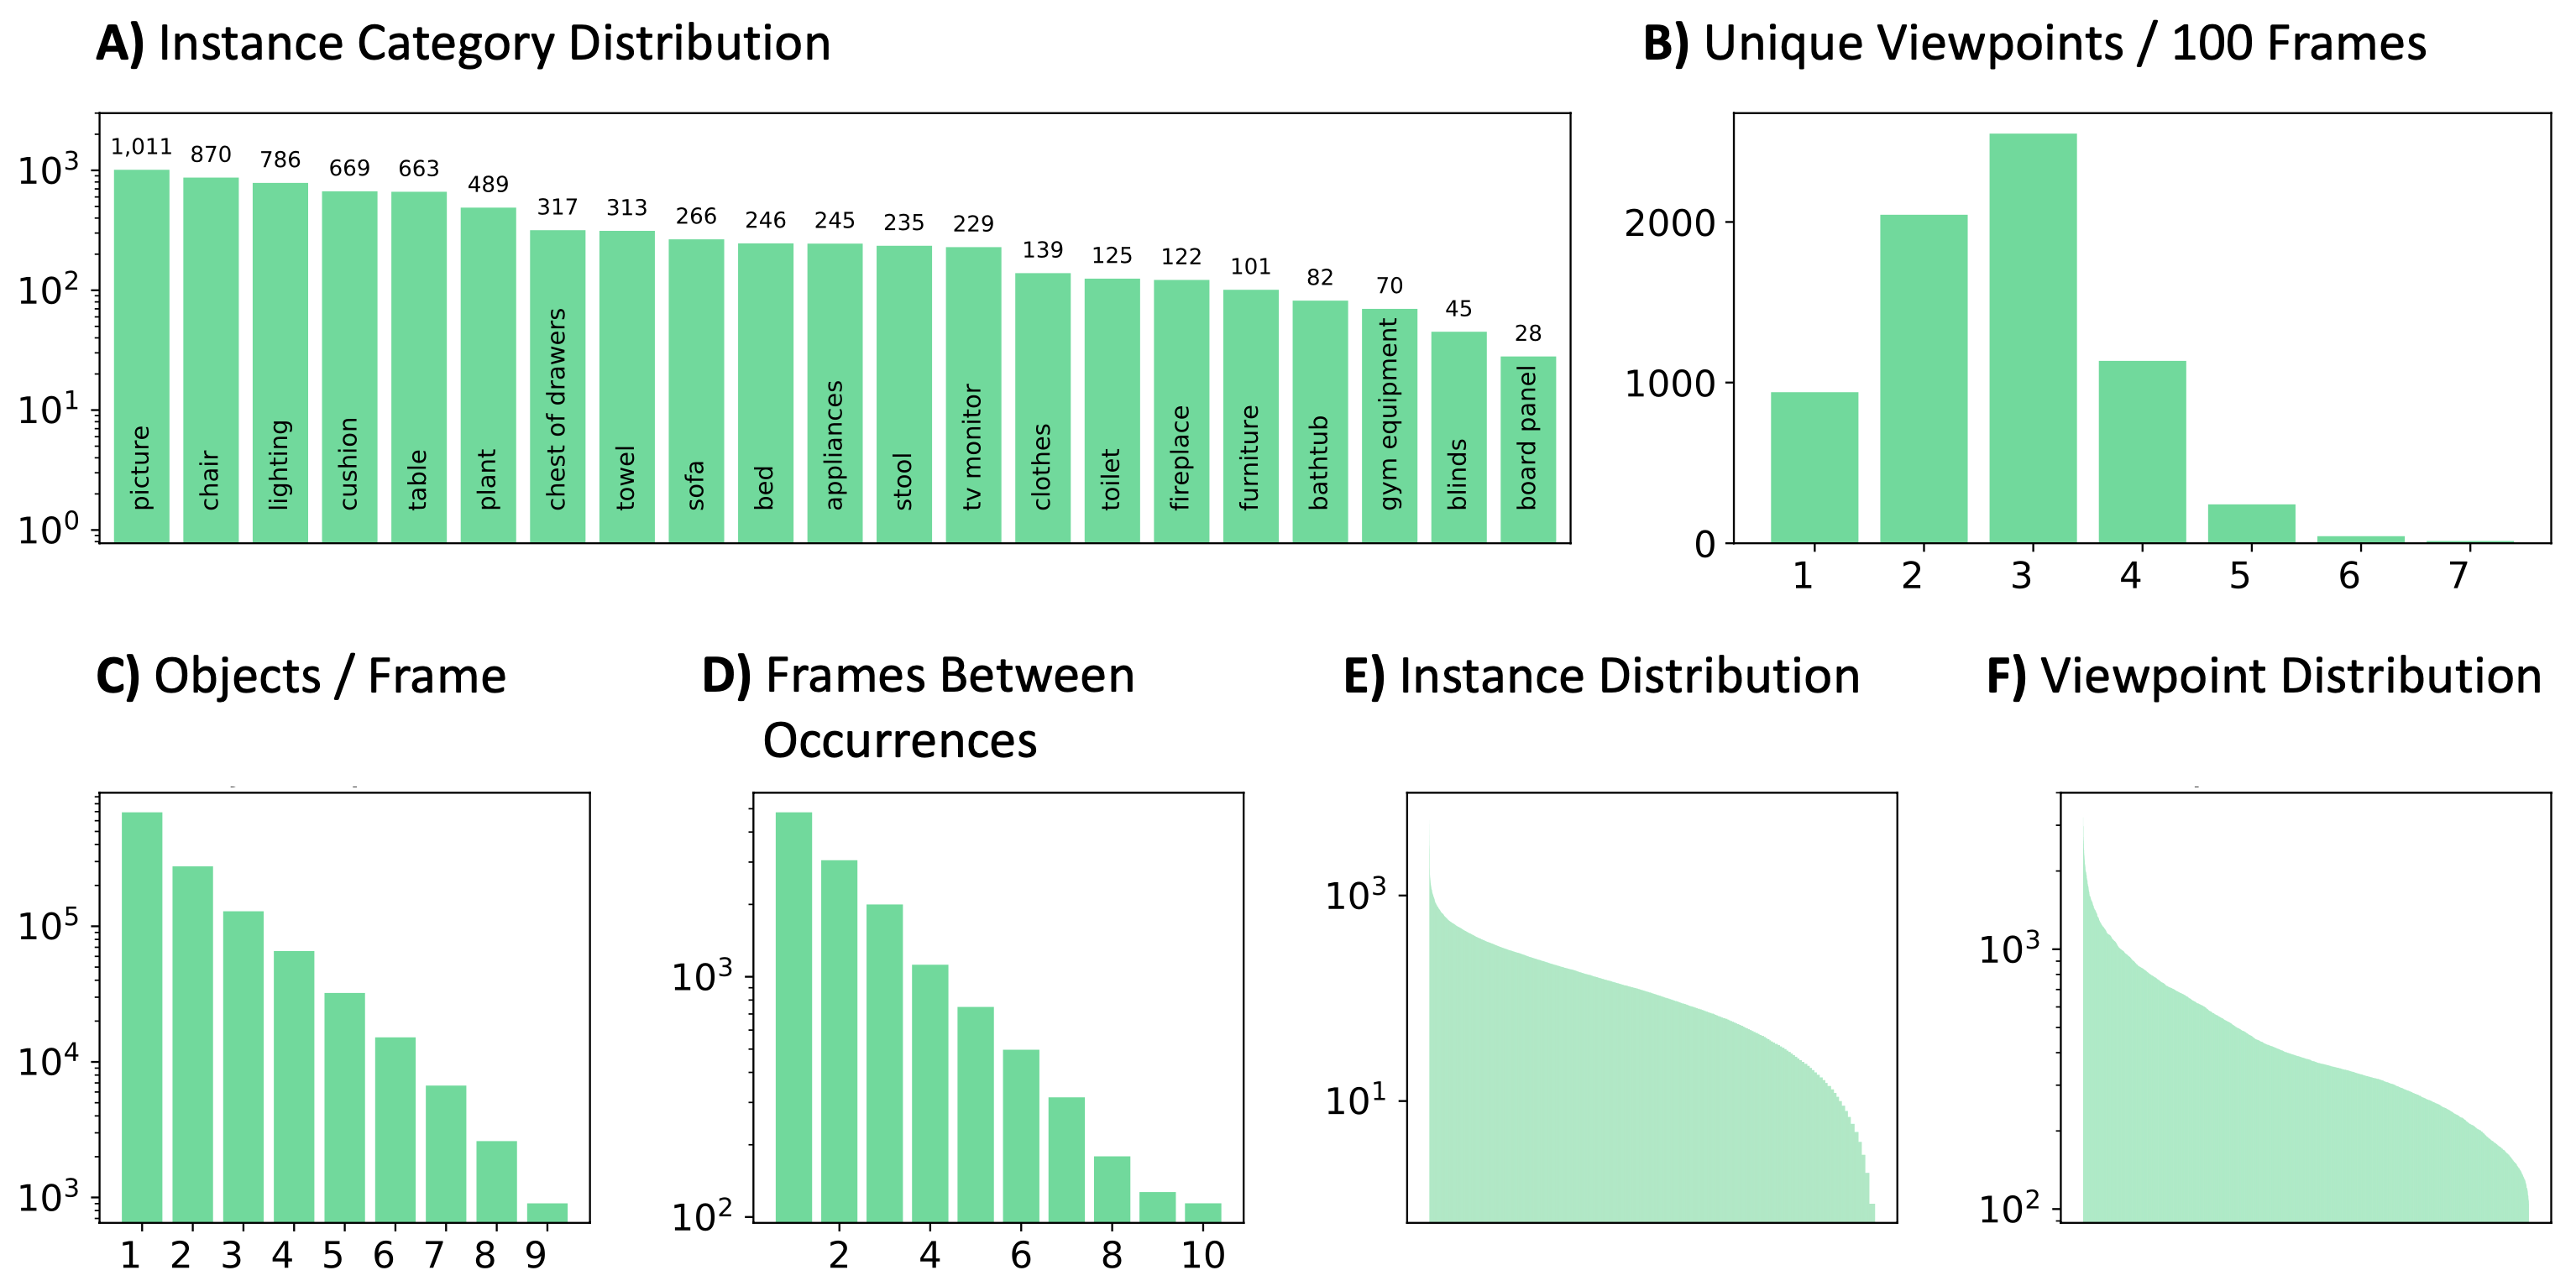
\includegraphics[width=6\textwidth]{figures/statsfull.png}
\else
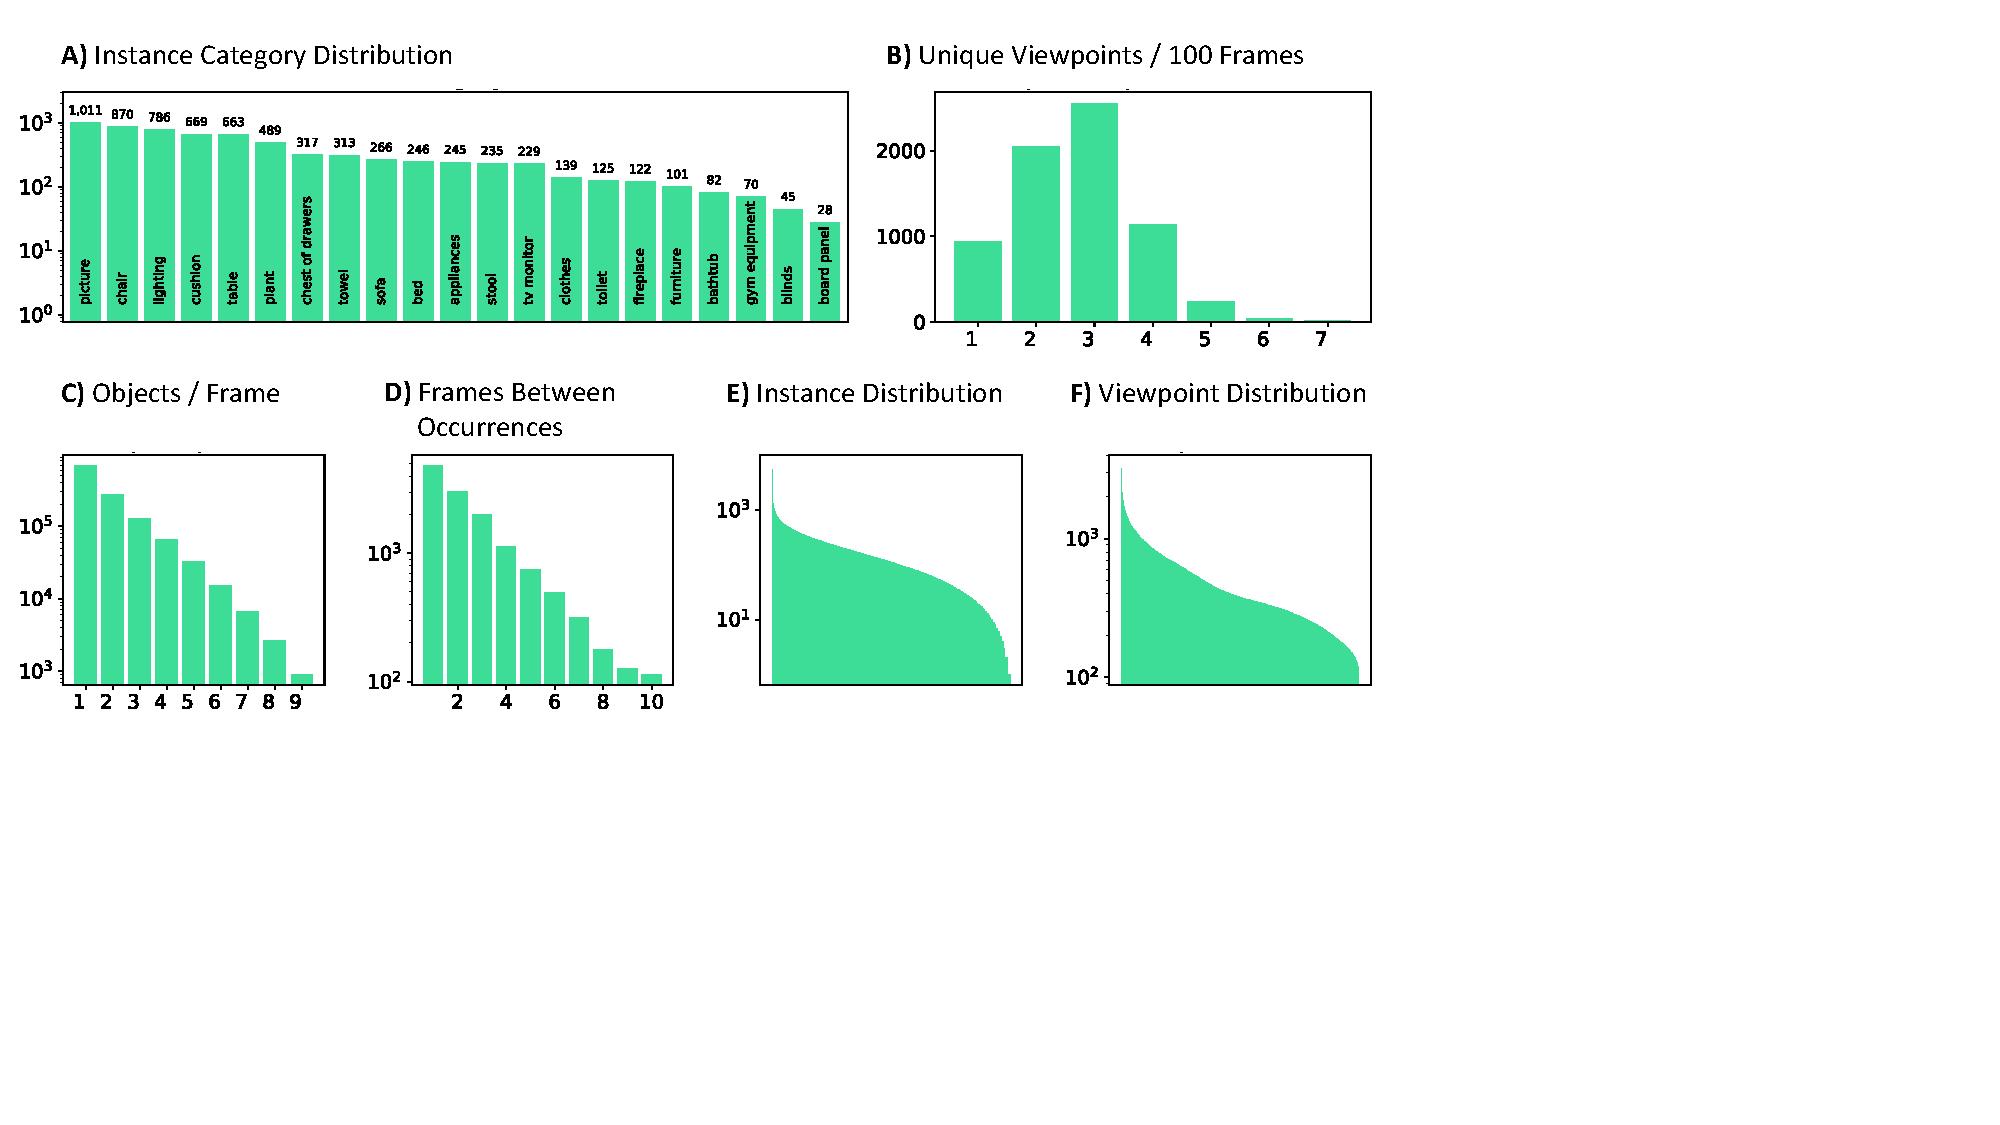
\includegraphics[width=0.9\textwidth,trim={0cm 7cm 10.2cm 0cm},clip]{figures/statsfull.pdf}
\fi
\caption{Additional statistics about our \ourroom{} dataset.}
\label{fig:additionalstats}
\end{figure}


\subsection{Training Procedure}
We use the Adam optimizer~\citep{adam} for all of our experiments, with a gradient cap of 5.0. For
\ourchar{} we train the network for 40k steps with a batch size 32 and maximum sequence length 150
across 2 GPUs and an initial learning rate 2e-3 decayed by 0.1$\times$ at 20k and 30k steps. For
\ourroom{} we train for 20k steps with a batch size 8 and maximum sequence length 100 across 4 GPUs
and an initial learning rate 1e-3 decayed by 0.1$\times$ at 8k and 16k steps. We use the BCE coefficient
$\lambda=1$  for all experiments. In semi-supervised experiments, around 30\% examples are labeled when the number of examples grows large ($\alpha = 0.3$, see Equation~\ref{eq:semisup}). Early stopping is used in \ourroom{} experiments
where the checkpoint with the highest validation AP score is chosen.
For \ourroom{}, we sample Bernoulli sequences on unlabeled inputs to 
gradually allow semi-supervised writing to the prototype memory and we find it helps training stability. The probability starts with 0.0 and increase by 0.2 every 2000 training steps until reaching 1.0.

\subsection{Data Augmentation}
For \ourchar{}, we pad the 28$\times$28 image to 32$\times$32 and then apply random cropping.

For \ourroom{}, we apply random cropping in the time dimension to get a chunk of 100 frames per
input example. We also apply random dropping of 5\% of the frames. We pad the 120$\times$160 images
to 126 $\times$ 168 and apply random cropping in each image frame. We also randomly flip the order
of the sequence (going forward or backward).


\subsection{Spatiotemporal context experiment details}
We use the Kylberg texture dataset~\citep{uppsala} without rotations. Texture classes are split into train, val, and test, defined in Table~\ref{tab:uppsalasplit}. We resize all images first to 256$\times$256. For each Omniglot image, a 28$\times$28 patch is randomly cropped from a texture image to serve as background. Random Gaussian noises with mean zero and standard deviation 0.1 are added to the background images.

For spatial background experiments, we added an additional learnable network of the same size as the main network to take the background image as input, and output the same sized embedding vector. This embedding vector is further concatenated with the main embedding vector to form the final embedding of the input. We also found that using spatially overlayed images with a single CNN can achieve similar performance as well. The final numbers are reported using the concatenation approach since it is less prone to overlay noises and is more similar to the implementation we use in the RoamingRooms experiments.

% !TEX root = ../supp.tex
\iflatexml
    \begin{table}[t]
    \begin{tabular}{clllll}
    \toprule

    \mr{3}{Train} &
    \texttt{blanket2} &
    \texttt{ceiling2} &
    \texttt{floor2} &
    \texttt{grass1} &
    \texttt{linseeds1} \\
    &
    \texttt{pearlsugar1} &
    \texttt{rice2} &
    \texttt{scarf2} &
    \texttt{screen1} &
    \texttt{seat2} \\
    &
    \texttt{sesameseeds1} &
    \texttt{stone1} & 
    \texttt{stoneslab1} & &
    \\
    \midrule

    \mr{2}{Val} &
    \texttt{blanket1} &
    \texttt{canvas1} &
    \texttt{ceiling1} & 
    \texttt{floor1} &
    \texttt{scarf1} \\
    &
    \texttt{rice1} &
    \texttt{stone2} & & & \\
    \midrule
    \mr{2}{Test} & 
    \texttt{wall1} &
    \texttt{lentils1} & 
    \texttt{cushion1} &
    \texttt{rug1} &
    \texttt{sand1} \\
    &
    \texttt{oatmeal1} &
    \texttt{stone3} &
    \texttt{seat1} & & \\
    \bottomrule
    \end{tabular}
    \caption{\textbf{Split information for the Kylberg texture dataset}. Each column is an texture type. Rows are continuation of lines.}
    \label{tab:uppsalasplit}
    \end{table}
\else
    \begin{table}[t]
    \vspace{-0.5in}
    \caption{\textbf{Split information for the Kylberg texture dataset}. Each column is an texture type. Rows are continuation of lines.}
    \label{tab:uppsalasplit}
    \begin{center}
    \begin{small}
    \begin{tabular}{clllll}
    \toprule

    \mr{3}{Train} &
    \texttt{blanket2} &
    \texttt{ceiling2} &
    \texttt{floor2} &
    \texttt{grass1} &
    \texttt{linseeds1} \\
    &
    \texttt{pearlsugar1} &
    \texttt{rice2} &
    \texttt{scarf2} &
    \texttt{screen1} &
    \texttt{seat2} \\
    &
    \texttt{sesameseeds1} &
    \texttt{stone1} & 
    \texttt{stoneslab1} & &
    \\
    \midrule

    \mr{2}{Val} &
    \texttt{blanket1} &
    \texttt{canvas1} &
    \texttt{ceiling1} & 
    \texttt{floor1} &
    \texttt{scarf1} \\
    &
    \texttt{rice1} &
    \texttt{stone2} & & & \\
    \midrule
    \mr{2}{Test} & 
    \texttt{wall1} &
    \texttt{lentils1} & 
    \texttt{cushion1} &
    \texttt{rug1} &
    \texttt{sand1} \\
    &
    \texttt{oatmeal1} &
    \texttt{stone3} &
    \texttt{seat1} & & \\
    \bottomrule
    \end{tabular}
    \end{small}
    \end{center}
    \end{table}
 \fi


\subsection{Baseline implementation details}
\paragraph{Online meta-learning (OML):} The OML  model performs one gradient descent step for each
input. In order for the model to predict unknown, we use the probability output from the softmax
layer summing across the unused units. For example, if the softmax layer has 40 units and we have
only seen 5 classes so far, then we sum the probability from the 6th to the last units. This summed
probability is separately trained with a binary cross entropy, same as in Equation~\ref{eq:loss}.

The inner learning rate is set to 1e-2 and we truncate the number of unrolled gradient descent steps
to 5/20 (\ourchar{}/\ourroom{}), in order to make the computation feasible. For \ourchar{}, the
network is trained with a batch size 32 across 2 GPUs, for a total of 20k steps, with an initial
learning rate 2e-3 decayed by 0.1 at 10k and 16.7k steps. For \ourroom{}, the network is trained
with a batch size 8 across 4 GPUs, for a total of 16k steps, with an initial learning rate 1e-3
decayed by 0.1 at 6.4k and 12.8k steps.

\paragraph{Long short-term memory (LSTM):} We apply a stacked two layer LSTM with 256 hidden
dimensions. Inputs are $\bh_t^{\text{CNN}}$ concatenated with the label one-hot vector. If an
example is unlabeled, then the label vector is all-zero. We directly apply a linear layer on top of
the LSTM to map the LSTM memory output into classification logits, and the last logit is the binary
classification logit reserved for unknown. The training procedure is the same as our CPM model.

\paragraph{Differentiable neural computer (DNC):} In order to make the DNC model work properly, we
found that it is sometimes helpful to pretrain the CNN weights. Simply initializing from scratch and
train CNN+DNC end-to-end sometimes results in poor performance. We hypothesize that the attention
structure in the DNC model is detrimental to representation learning. Therefore, for \ourchar{}
experiments, we use pretrained ProtoNet weights for solving 1-shot 5-way episodes to initialize the
CNN, and we keep finetuning the CNN weights with 10\% of the full learning rate. For \ourroom{}
experiments, we train the full model end-to-end from scratch.

The DNC is also modified so that it is more effective using the label information from the input. In
the original MANN paper~\citep{mann} for one-shot learning, the input features $\bh_t^{\text{CNN}}$
and the label one-hot ID are simply concatenated to feed into the LSTM controller of MANN. We find
that it is beneficial to directly add label one-hot vector as an input to the write head that
generates the write attention and the write content.  Similar to the LSTM model, the memory readout is also sent to a
linear layer in order to get the final classification logits, and the last logit is the binary
classification logit reserved for the unknowns. Finally we remove the linkage prediction part of the DNC
due to training instability.

The controller LSTM has 256 hidden dimensions, and the memory has 64 slots each with 64 dimensions.
There are 4 read heads and 4 write heads. The training procedure is the same as CPM.

\paragraph{Online ProtoNet:} Online ProtoNet is our modification of the original
ProtoNet~\citep{protonet}. It is similar to our CPM model without the contextual RNN. The feature
from the CNN is directly written to the prototype memory. In addition, we do not predict the control
hyperparameters $\beta^{\{r,w\}}_t,\gamma^{\{r,w\}}_t$ from the RNN and they are learned as regular parameters. The training procedure is the same as CPM.

\paragraph{Online MatchingNet:} Online MatchingNet is our modification of the original
MatchingNet~\citep{matchingnet}. We do not consider the context embedding in the MatchingNet paper
since it was originally designed for the entire episode using an attentional RNN encoder. It is
similar to online ProtoNet but instead of doing online averaging, it directly stores each example
and its class. Since it is an example-based storage, we did not extend it to learn from
unlabeled examples, and all unlabeled examples are skipped. We use a similar decision rule to
determine whether an example belongs to a known cluster by looking at the distance to the nearest
exemplar stored in the memory, shifted by $\beta$ and scaled by $1/\gamma$. Note that online
MatchingNet is not efficient at memory storage since it scales with the number of steps in the
sequence. In addition, we use the negative Euclidean distance as the similarity function. The training
procedure is the same as CPM.

\paragraph{Online infinite mixture prototypes (IMP):} Online IMP is proposed as a mix of prototype and example-based storage by allowing a class to have multiple clusters. If an
example is classified as unknown or it is unlabeled, we will assign its cluster based on our
prediction, which either assigns it to one of the existing clusters or creates a new cluster,
depending on its distance to the nearest cluster. If a cluster with an unknown label later is
assigned with an example with a known class, then the cluster label will also be updated. We use the same
decision rule as online ProtoNet to determine whether an example belongs to a known cluster by
looking at the distance to the nearest cluster, shifted by $\beta$ and scaled by $1/\gamma$. As
described above, online IMP has the capability of learning from unlabeled examples, unlike online
MatchingNet. However similar to online MatchingNet, online IMP is also not efficient at memory
storage since in the worst case it also scales with the number of steps in the sequence. Again, the
training procedure is the same as CPM.

\section{Additional Experimental Results}
\label{sec:additionalresults}
\subsection{Effect of Forgetting}
We report the effect of forgetting of \ourroom{} and \ourimg{} in Table~\ref{tab:forgetroom} and \ref{tab:forgetimagenet}.
\iflatexml
\begin{table}[t]
    \centering
    \begin{tabular}{ccccccc|cccccc}
    \toprule
    & \mc{6}{c|}{\textbf{Supervised}} & \mc{6}{c}{\textbf{Semi-Supervised}}\\
                &   1 - 2&      3 - 5&      6 - 10&     11 - 20&    21 - 50&    51 - 100&
                    1 - 2&      3 - 5&      6 - 10&     11 - 20&    21 - 50&    51 - 100\\
    OPN 1-Shot  &   93.5&   	89.3&	    79.4&	    67.2&	    60.3&	    60.1&
                    86.5&	    83.6&	    76.3&	    68.4&	    64.7&	    61.5\\
    CPM 1-Shot  &   \bf{95.7}&	\bf{92.2}&  \bf{85.7}&	\bf{75.2}&	\bf{70.0}&  \bf{66.4}&
                    \bf{91.0}&	\bf{88.7}&	\bf{82.9}&	\bf{77.0}&  \bf{72.2}&	\bf{66.5}\\
    OPN 3-Shot  &   95.1&	    91.8&	    85.6&   	78.2&	    74.6&	    73.8&
                    92.6&       88.0&	    85.1&	    81.1&	    80.6&	    76.7\\
    CPM 3-Shot  &   \bf{96.1}&	\bf{93.8}&	\bf{87.7}&	\bf{81.4}&  \bf{79.1}&	\bf{78.2}&
                    \bf{94.8}&  \bf{91.0}&	\bf{86.9}&	\bf{83.1}&	\bf{82.7}&  \bf{79.2}\\
    \bottomrule
    \end{tabular}
    \caption{\textbf{Effect of forgetting over a time interval on \ourroom{}.} Average accuracy vs. the number of time steps since the model has last seen the label of a particular class.}
    \label{tab:forgetroom}
\end{table}

\begin{table}[t]
    \centering
    \begin{tabular}{ccccccc|cccccc}
    \toprule
    & \mc{6}{c|}{\bf Supervised} & \mc{6}{c}{\bf Semi-Supervised}\\
                &   1 - 2&      3 - 5&      6 - 10&     11 - 20&    21 - 50&    51 - 100&
                    1 - 2&      3 - 5&      6 - 10&     11 - 20&    21 - 50&    51 - 100\\
    OPN 1-Shot  &   40.8&	35.9&	33.0&	\bf{30.7}&	\bf{27.0}&	\bf{21.4}&
                    40.5&	37.7&	35.9&	\bf{33.7}&	\bf{31.5}&	\bf{28.4}\\
    CPM 1-Shot  &   \bf{67.5}&	\bf{52.9}&	\bf{35.5}&	24.2&	18.3&	13.8&
                    \bf{60.4}&	\bf{51.3}&	\bf{39.5}&	26.6&	21.8&	15.4\\
    OPN 3-Shot  &   52.5&	50.3&	\bf{48.8}&	\bf{47.2}&	\bf{44.4}&	\bf{42.3}&
                    57.6&	55.1&	\bf{54.6}&	\bf{52.3}&	\bf{52.1}&	\bf{49.5}\\
    CPM 3-Shot  &   \bf{77.8}&	\bf{64.5}&	46.6&	32.9&	24.7&	17.9&
                    \bf{76.1}&	\bf{61.8}&	48.6&	30.5&	24.1&	15.6\\
    \bottomrule
    \end{tabular}
    \caption{\textbf{Effect of forgetting over a time interval on \ourimg{}.} Average accuracy vs. the number of time steps since the model has last seen the label of a particular class.}
    \label{tab:forgetimagenet}
\end{table}

\else
\begin{table}[t]
\vspace{-0.5in}
    \centering
    \caption{\textbf{Effect of forgetting over a time interval on \ourroom{}.} Average accuracy vs. the number of time steps since the model has last seen the label of a particular class.}
    
    \resizebox{\textwidth}{!}{
    \begin{tabular}{ccccccc|cccccc}
    \toprule
    & \mc{6}{c}{\bf Supervised} & \mc{6}{c}{\bf Semi-Supervised}\\
                &   1 - 2&      3 - 5&      6 - 10&     11 - 20&    21 - 50&    51 - 100&
                    1 - 2&      3 - 5&      6 - 10&     11 - 20&    21 - 50&    51 - 100\\
    \midrule
    OPN 1-Shot  &   93.5&   	89.3&	    79.4&	    67.2&	    60.3&	    60.1&
                    86.5&	    83.6&	    76.3&	    68.4&	    64.7&	    61.5\\
    CPM 1-Shot  &   \bf{95.7}&	\bf{92.2}&  \bf{85.7}&	\bf{75.2}&	\bf{70.0}&  \bf{66.4}&
                    \bf{91.0}&	\bf{88.7}&	\bf{82.9}&	\bf{77.0}&  \bf{72.2}&	\bf{66.5}\\
    \midrule
    OPN 3-Shot  &   95.1&	    91.8&	    85.6&   	78.2&	    74.6&	    73.8&
                    92.6&       88.0&	    85.1&	    81.1&	    80.6&	    76.7\\
    CPM 3-Shot  &   \bf{96.1}&	\bf{93.8}&	\bf{87.7}&	\bf{81.4}&  \bf{79.1}&	\bf{78.2}&
                    \bf{94.8}&  \bf{91.0}&	\bf{86.9}&	\bf{83.1}&	\bf{82.7}&  \bf{79.2}\\
    \bottomrule
    \end{tabular}}
    \label{tab:forgetroom}
\end{table}

\begin{table}[t]
\vspace{-0.2in}
    \centering
    \caption{\textbf{Effect of forgetting over a time interval on \ourimg{}.} Average accuracy vs. the number of time steps since the model has last seen the label of a particular class.}
    
    \resizebox{\textwidth}{!}{
    \begin{tabular}{ccccccc|cccccc}
    \toprule
    & \mc{6}{c}{\bf Supervised} & \mc{6}{c}{\bf Semi-Supervised}\\
                &   1 - 2&      3 - 5&      6 - 10&     11 - 20&    21 - 50&    51 - 100&
                    1 - 2&      3 - 5&      6 - 10&     11 - 20&    21 - 50&    51 - 100\\
    \midrule
    OPN 1-Shot  &   40.8&	35.9&	33.0&	\bf{30.7}&	\bf{27.0}&	\bf{21.4}&
                    40.5&	37.7&	35.9&	\bf{33.7}&	\bf{31.5}&	\bf{28.4}\\
    CPM 1-Shot  &   \bf{67.5}&	\bf{52.9}&	\bf{35.5}&	24.2&	18.3&	13.8&
                    \bf{60.4}&	\bf{51.3}&	\bf{39.5}&	26.6&	21.8&	15.4\\
    \midrule
    OPN 3-Shot  &   52.5&	50.3&	\bf{48.8}&	\bf{47.2}&	\bf{44.4}&	\bf{42.3}&
                    57.6&	55.1&	\bf{54.6}&	\bf{52.3}&	\bf{52.1}&	\bf{49.5}\\
    CPM 3-Shot  &   \bf{77.8}&	\bf{64.5}&	46.6&	32.9&	24.7&	17.9&
                    \bf{76.1}&	\bf{61.8}&	48.6&	30.5&	24.1&	15.6\\
    \bottomrule
    \end{tabular}}
    \label{tab:forgetimagenet}
\end{table}


% \subsection{Video Visualization}
% We include video visualization of \ourroom{} sequences here:
% \footnote{\url{https://drive.google.com/drive/folders/1gBJBFdNb0EOvK6CEYKxIL1Og0_jrqrbK}}. Our CPM
% model prediction can be found here:
% \footnote{\url{https://drive.google.com/drive/folders/1rp9xxAccrZyffngFdtoS9Bl6P9uxJ9xN}}.

\subsection{Embedding Visualization} 
Figure~\ref{fig:tsne} shows the learned embedding of each example in Online ProtoNet vs. our CPM
model in \ourchar{} sequences, where colors indicate environment IDs. In Online ProtoNet, the
example features does not reflect the temporal context, and as a result, colors are scattered across
the space. By contrast, in the CPM embedding visualization, colors are clustered together and we see
a smoother transition of environments in the embedding space.

% !TEX root = ../supp.tex
\begin{figure}[t]
\centering
% \vspace{-0.2in}
\iflatexml
    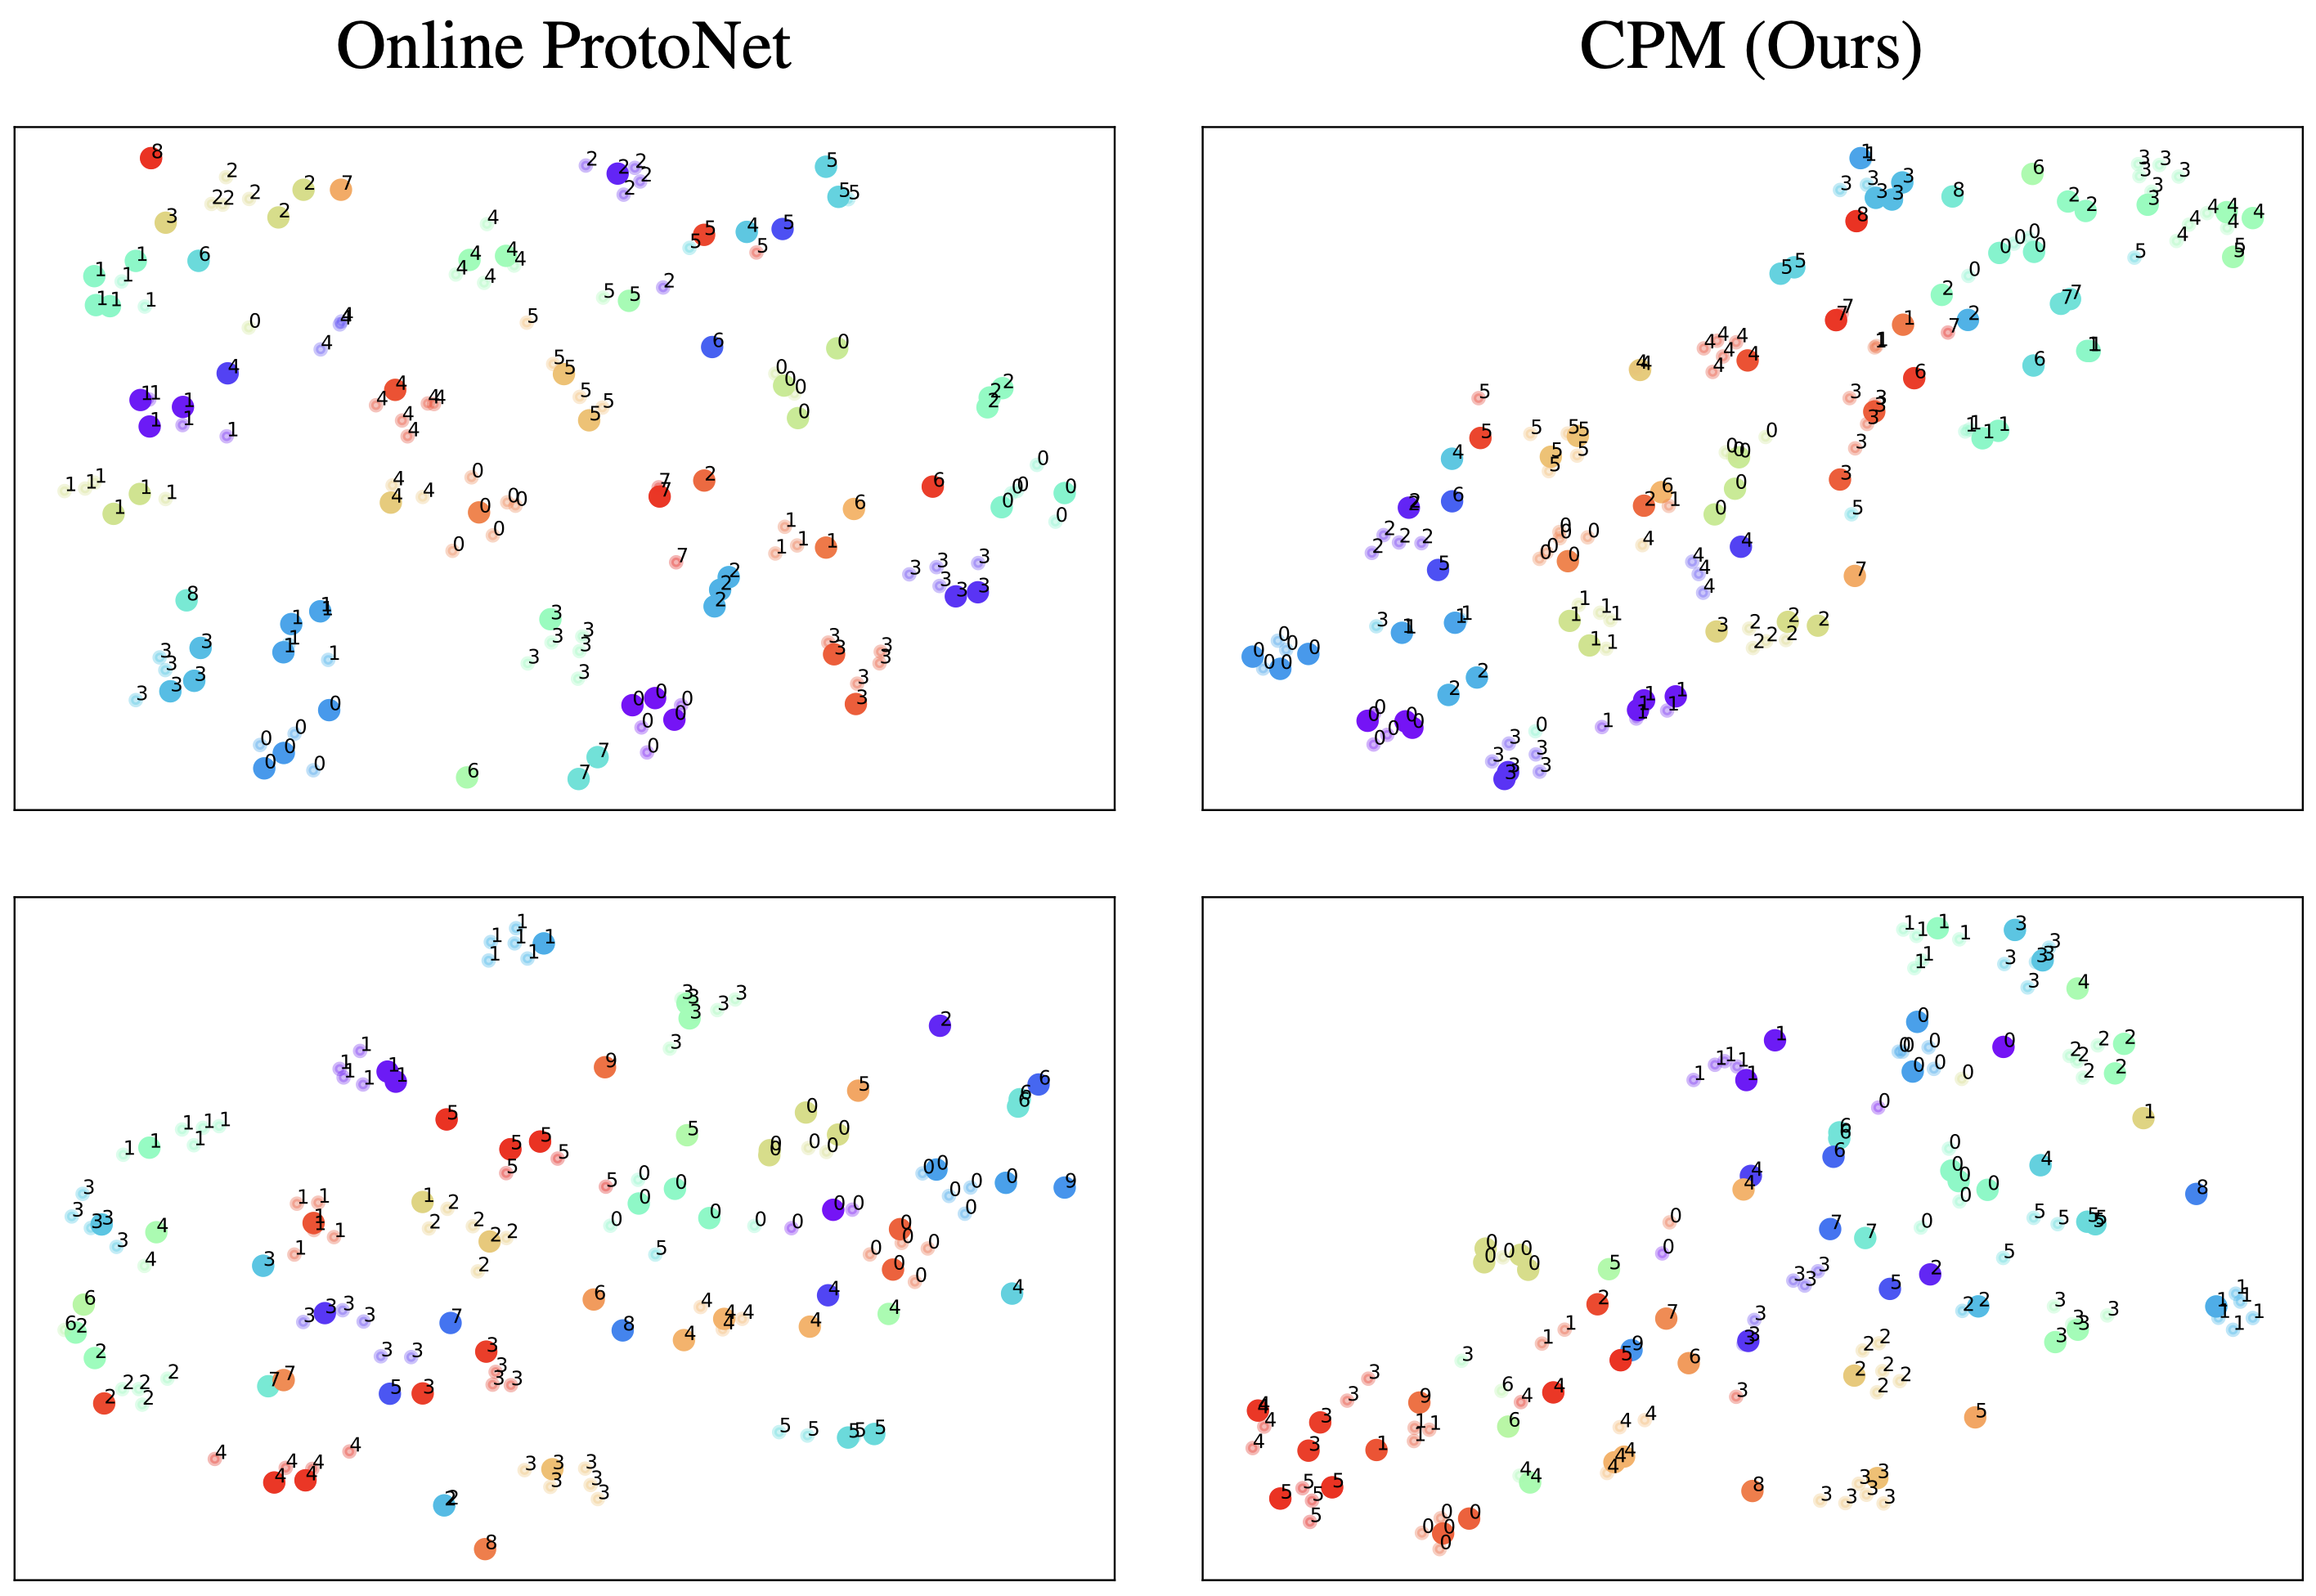
\includegraphics[width=6\linewidth]{figures/omniglot-tsne.png}
\else
    \begin{tabular}{cc}
    Online ProtoNet & CPM (Ours) \\
    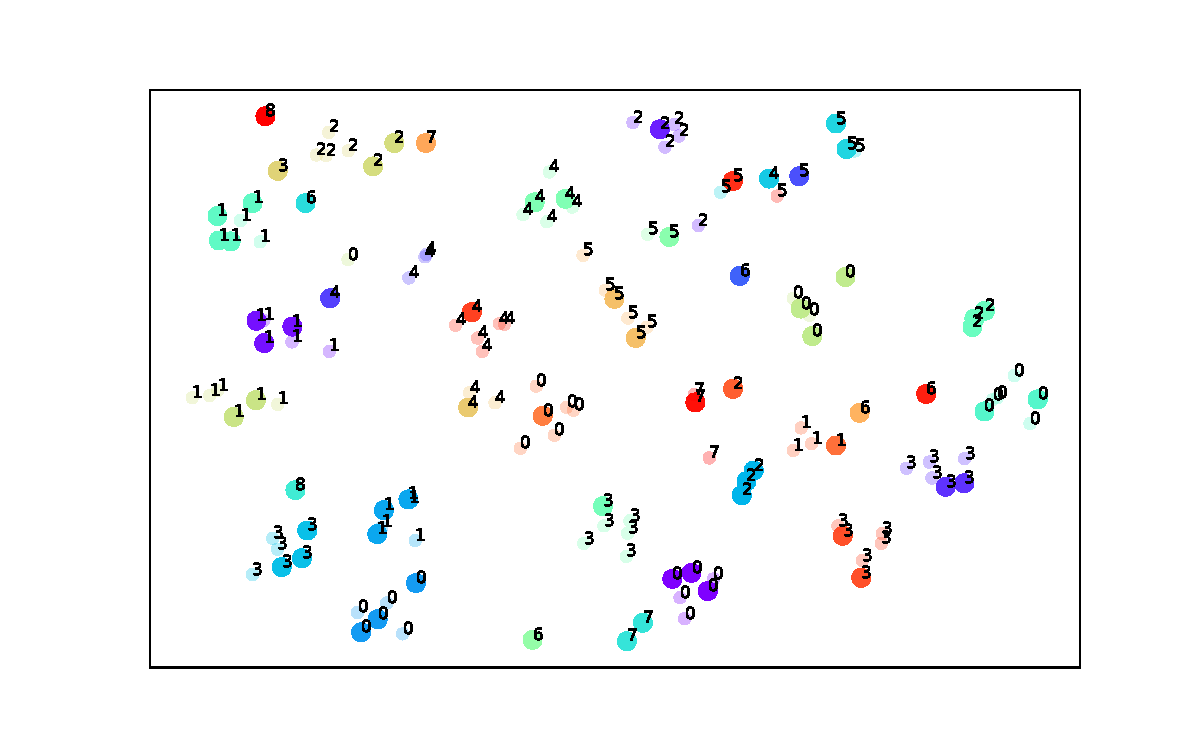
\includegraphics[height=3.8cm, trim={2.5cm 1cm 2cm 1cm}, clip]{figures/omniglot-protonet-tsne/tsne-003.pdf}
    &
    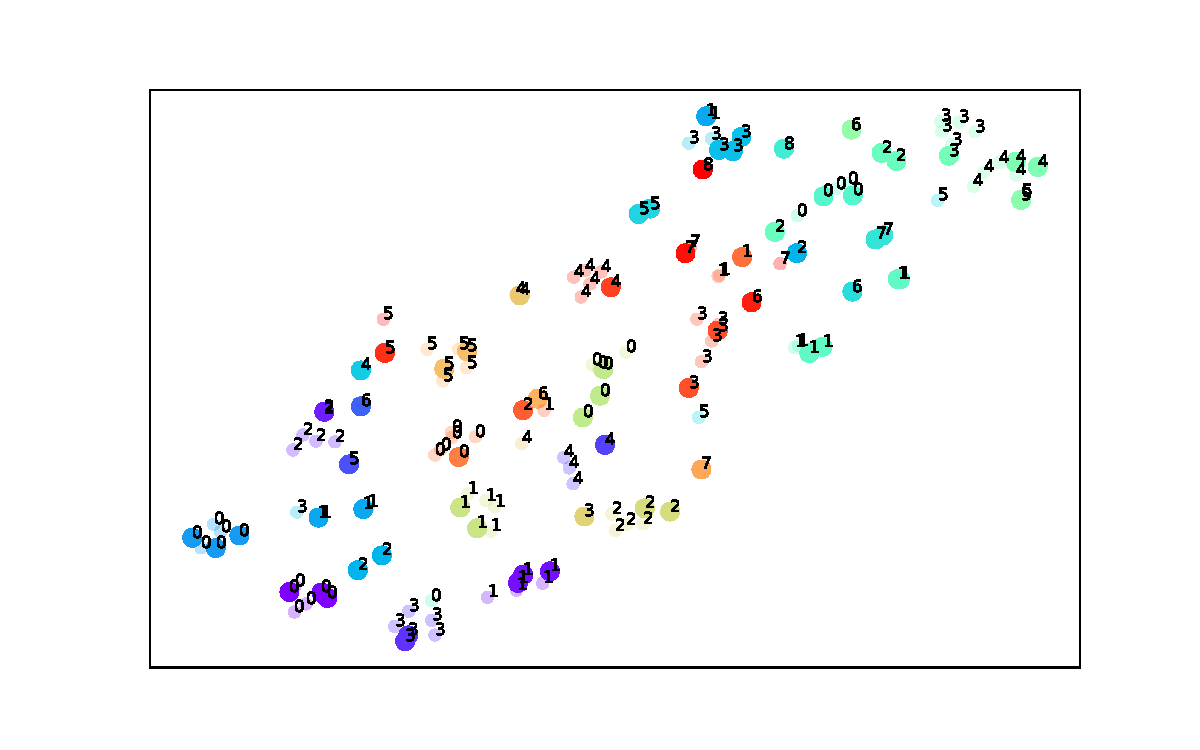
\includegraphics[height=3.8cm, trim={2.5cm 1cm 2cm 1cm}, clip]{figures/omniglot-cpm-tsne/tsne-003.pdf}
    \\
    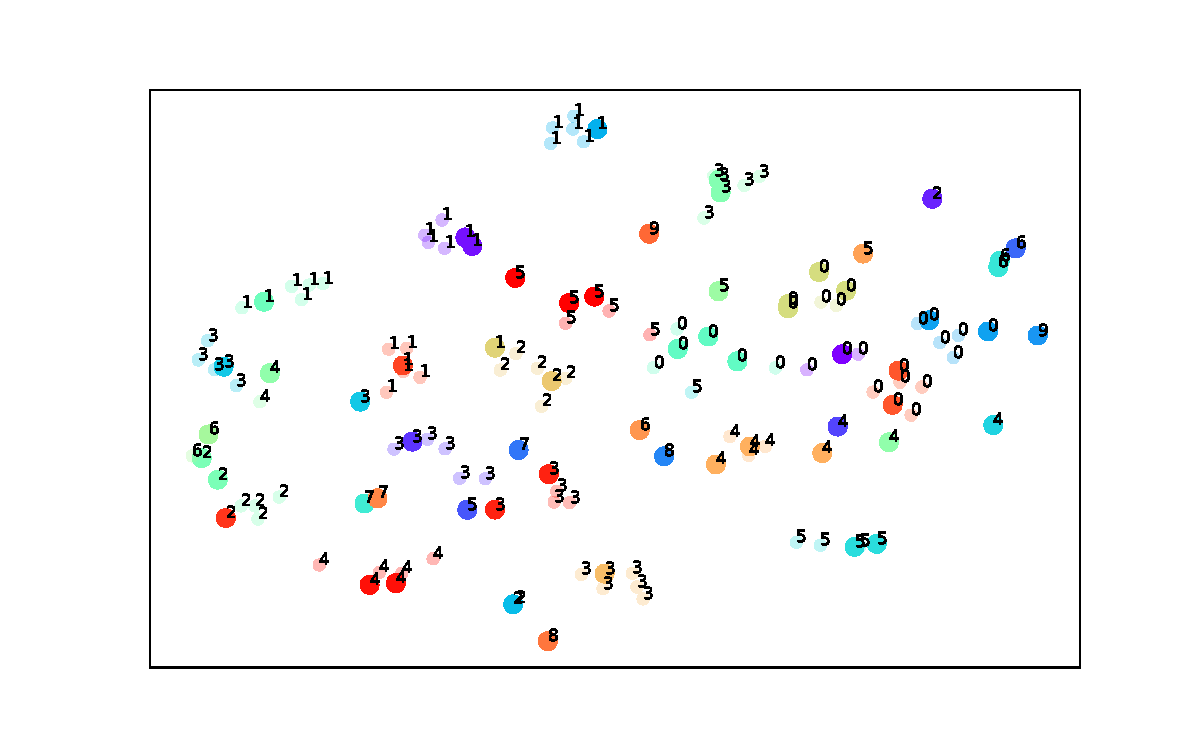
\includegraphics[height=3.8cm, trim={2.5cm 1cm 2cm 1cm}, clip]{figures/omniglot-protonet-tsne/tsne-008.pdf}
    &
    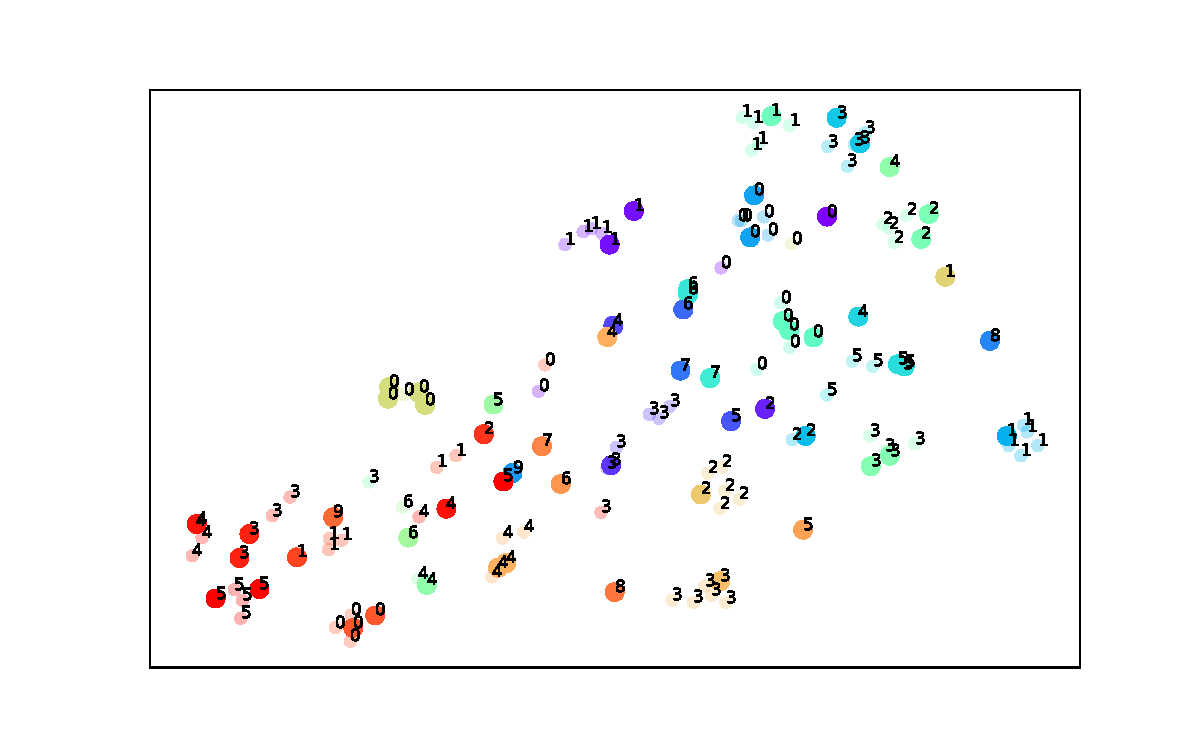
\includegraphics[height=3.8cm, trim={2.5cm 1cm 2cm 1cm}, clip]{figures/omniglot-cpm-tsne/tsne-008.pdf}
    \end{tabular}
\fi
\caption{\textbf{Embedding space visualization of \ourchar{} sequences using t-SNE~\citep{tsne}}. Different color
denotes different environments. Text labels (relative to each environment) are annotated beside the
scatter points. Unlabeled examples shown in smaller circles with lighter colors. \textbf{Left:}
Online ProtoNet; \textbf{Right:} CPM. The embeddings learned CPM model shows a smoother transition
of classes based on their temporal environments.}
\label{fig:tsne}
\end{figure}


\subsection{Control Parameters vs. Time}
Finally we visualize the control parameter values predicted by the RNN in
Figure~\ref{fig:betagamma}. We verify that we indeed need two sets of $\beta$ and $\gamma$ for read
and write operations separately as they learn different values. $\beta^w$ is smaller than $\beta^r$
which means that the network is more conservative when writing to prototypes. $\gamma^w$ grows
larger over time, which means that the network prefers a softer slope when writing to prototypes
since in the later stage the prototype memory has already stored enough content and it can grow
faster, whereas in the earlier stage, the prototype memory is more conservative to avoid embedding
vectors to be assigned to wrong clusters.

% !TEX root = ../supp.tex
\begin{figure}
\centering
% \vspace{-0.1in}
\iflatexml
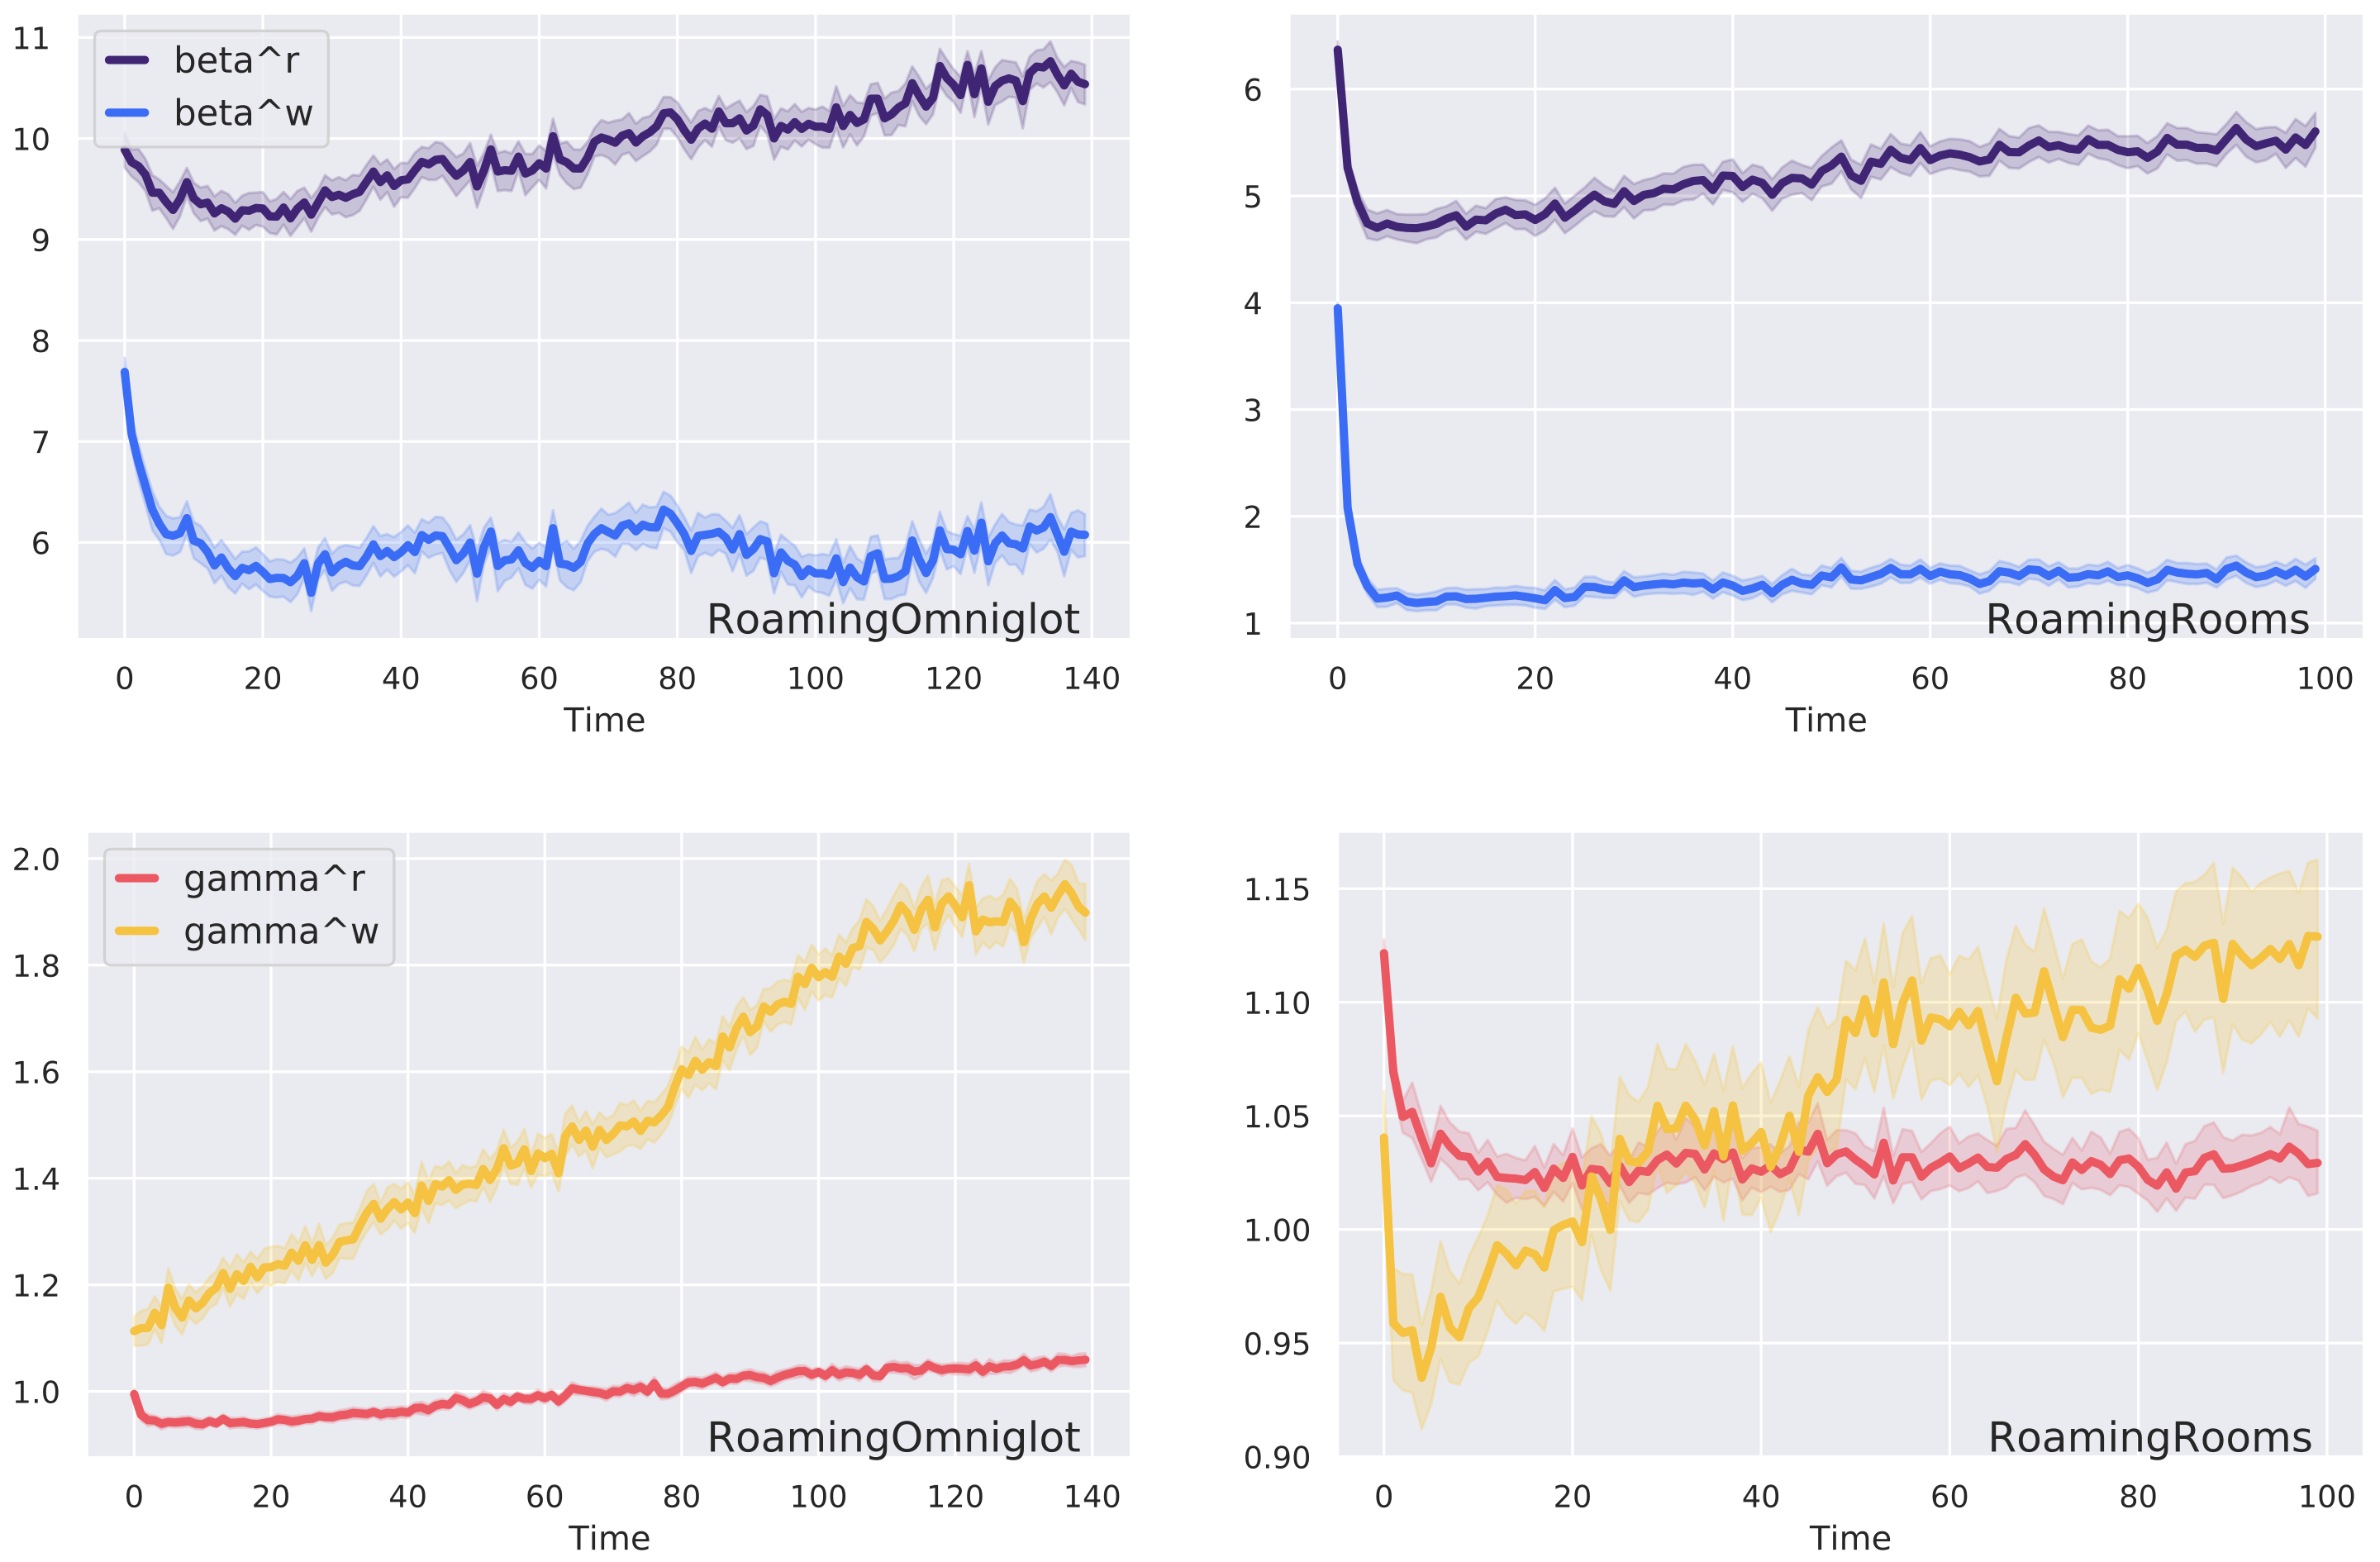
\includegraphics[width=6\linewidth]{figures/beta-gamma.png}
\else
\begin{tabular}{cc}
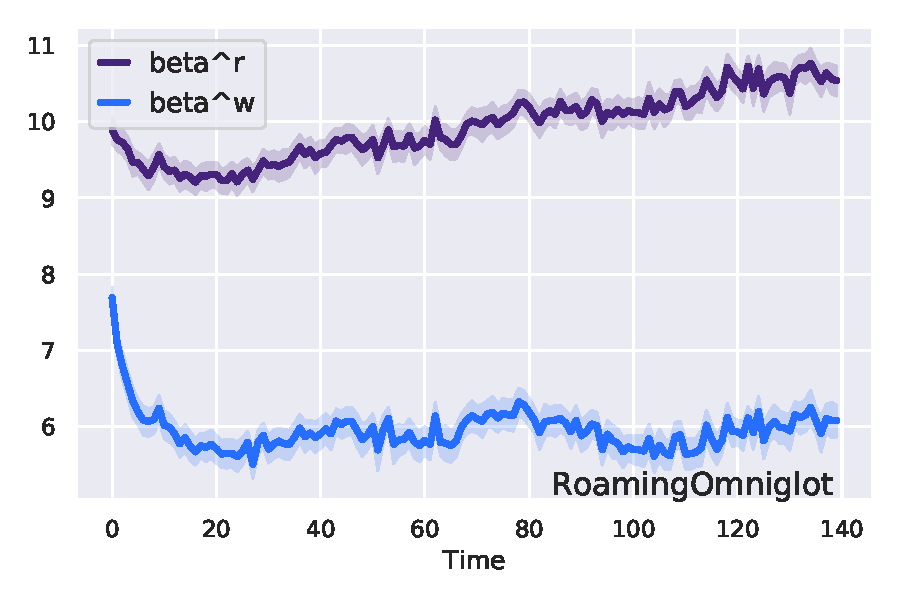
\includegraphics[height=4.0cm,trim={0.3cm 0cm 0.5cm 0},clip]{figures/omniglot-beta.pdf}
\quad
&
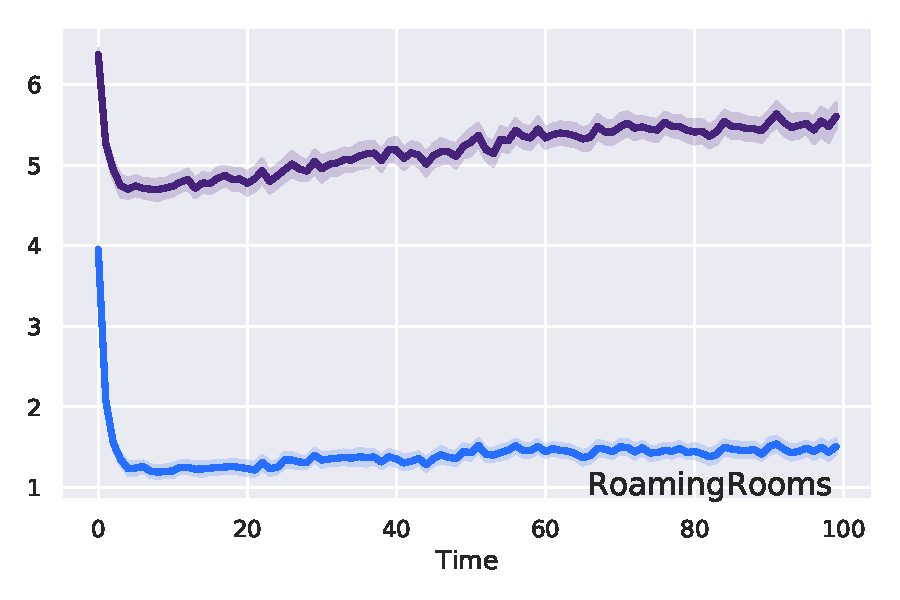
\includegraphics[height=4.0cm,trim={0.3cm 0cm 0cm 0},clip]{figures/matterport-beta.pdf}
\\
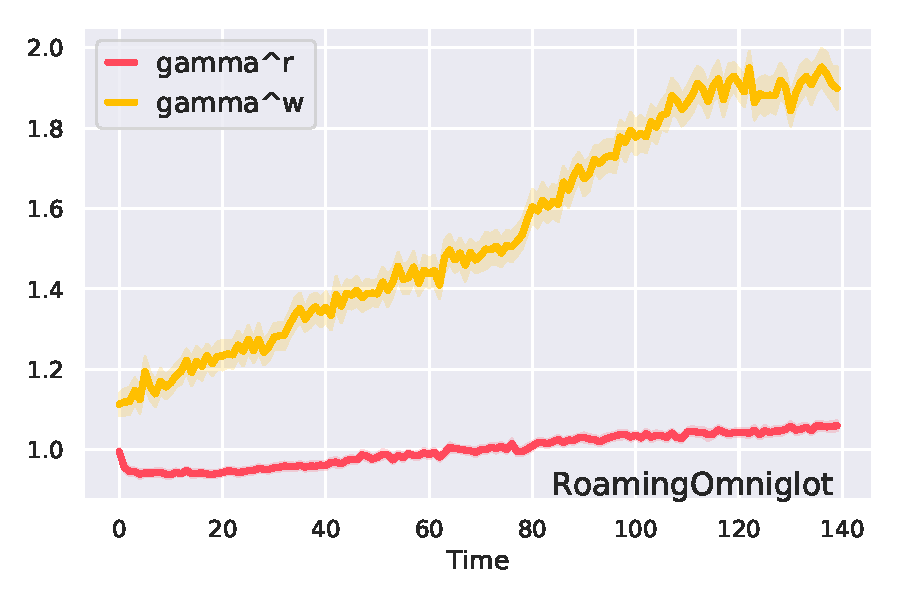
\includegraphics[height=4.0cm,trim={0.3cm 0cm 0.5cm 0},clip]{figures/omniglot-gamma.pdf}
\quad
&
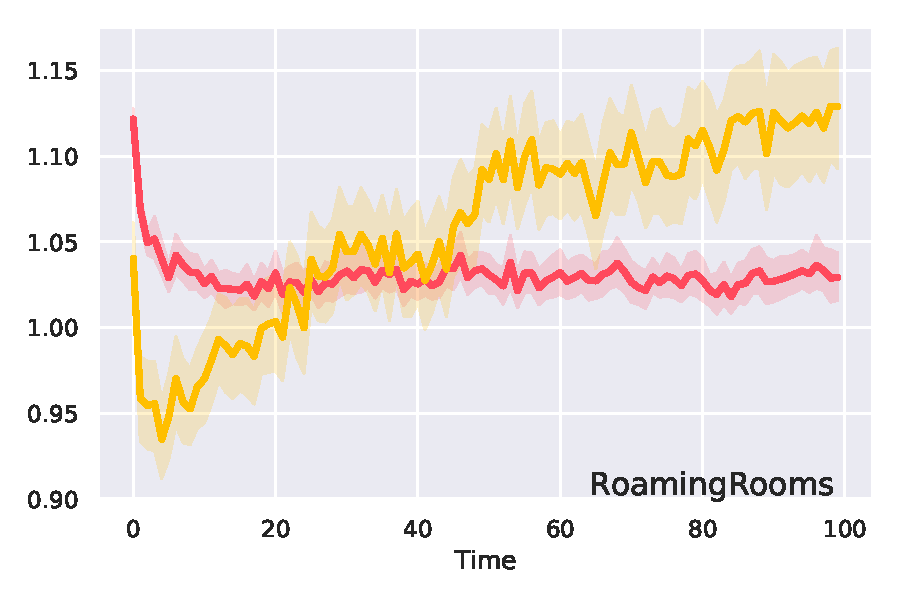
\includegraphics[height=4.0cm,trim={0.3cm 0cm 0cm 0},clip]{figures/matterport-gamma.pdf}
\\
\end{tabular}
\vspace{-0.1in}
\fi
\caption{\textbf{CPM control parameters ($\beta^{r,w}, \gamma^{r,w}$) vs. time.}
\textbf{Left:} \ourchar{} sequences; \textbf{Right:} \ourroom{} sequences; \textbf{Top:}
$\beta^{r,w}$ the threshold parameter; \textbf{Bottom:} $\gamma^{r,w}$ the temperature parameter.}
\label{fig:betagamma}
\end{figure}



\clearpage
\newpage
{
\setstretch{0.93}
\bibliography{ref}
\bibliographystyle{iclr2021_conference}
}

\setstretch{1.0}
\end{document}